\documentclass[11pt,a4paper,twoside,openright]{report}

\usepackage{graphicx}
\graphicspath{{./pictures/}}
\usepackage{tabularx}
\usepackage{subfigure}
\usepackage{afterpage}
\usepackage{amsmath,amssymb}            
\usepackage{rotating}  
\usepackage{fancyhdr}  
\usepackage[scriptsize]{caption} 
\usepackage{siunitx}
\usepackage{gensymb}
\usepackage{multirow}
\DeclareSIUnit{\EUR}{\text{\euro}}

\usepackage{algorithm}
\usepackage[noend]{algpseudocode}

\makeatletter
\def\BState{\State\hskip-\ALG@thistlm}
\makeatother

\hyphenation{a-gen-tiz-za-zio-ne}

\setlength{\paperwidth}{16cm}
\setlength{\paperheight}{24cm}
\setlength{\oddsidemargin} {2. cm}
\setlength{\evensidemargin} {2. cm}
\addtolength{\oddsidemargin} {-0.4 cm}
\addtolength{\evensidemargin} {-0.4 cm}
\linespread{1.1}

\usepackage[italian]{babel}
\usepackage[T1]{fontenc} 
\usepackage[utf8]{inputenc}
\renewcommand{\captionfont}{\normalfont \sffamily \itshape \small}

\pagestyle{empty}

\begin{document}
\thispagestyle{empty}
%\begin{titlepage}
\vspace*{-1.5cm} \bfseries{
\begin{center}
  \large
  POLITECNICO DI MILANO\\
  \normalsize
  Scuola di Ingegneria Industriale e dell'Informazione\\
  Corso di Laurea \textbf{MAGISTRALE} in Ingegneria Informatica\\
  \begin{figure}[htbp]
    \begin{center}
      
\includegraphics[width=5cm]{./pictures/frontesp/NewLogo.png}
%	
\psfig{file=./pictures/logopm.jpg,width=3.5cm}
    \end{center}
  \end{figure}
  \vspace*{0.3cm} \LARGE



  \textbf{Sviluppo firmware per misuratore laser di distanza basato su FPGA}\\



  \vspace*{.75truecm} \large
\end{center}
\vspace*{3.0cm} \large
\begin{flushleft}


  Relatore: Prof. Michele Norgia

\end{flushleft}
\vspace*{1.0cm}
\begin{flushright}


  Tesi di Laurea di:\\ Leonardo Cavagnis, matricola 816646 \\ 
		       Diego Rondelli, matricola 817108 \\


\end{flushright}
\vspace*{0.5cm}
\begin{center}



  Anno Accademico 2014-2015
\end{center} \clearpage
}

\thispagestyle{empty} \normalfont \cleardoublepage
\vspace{17cm}

%\large
\begin{flushright}
\itshape{Alle nostre famiglie...}
\end{flushright}

\thispagestyle{empty}  \cleardoublepage
\pagenumbering{Roman}
\newpage
\chapter*{Sommario}

\addcontentsline{toc}{chapter}{Sommario}
Lo scopo di questo lavoro di tesi \'e sviluppare il firmware di un misuratore laser basato sulla tecnica di interferometria a retroiniezione per misurare la distanza assoluta di un bersaglio.

La prima parte del lavoro consiste nell'implementazione del firmware, sviluppato usando NI LabVIEW FPGA e Real-Time, e degli algoritmi necessari per la misura della distanza assoluta.

Nella seconda perte ci si \'e concentrati sull'ottimizzazione degli algoritmi implementati e sulla calibrazione dei parametri di funzionamento del sistema, al fine di migliorare la precisione e l'accuratezza della misura.

\thispagestyle{empty}  \cleardoublepage
\newpage
\chapter*{Abstract}

\addcontentsline{toc}{chapter}{Abstract}

ToDO

\thispagestyle{empty} \vspace*{.75truecm} \cleardoublepage
\tableofcontents
\listoffigures
\listoftables
\thispagestyle{empty} \vspace*{.75truecm} \normalfont \cleardoublepage
\pagestyle{plain}\renewcommand{\chaptermark}[1]{\markboth{\chaptername\ \thechapter.\ #1}{}} 
\renewcommand{\sectionmark}[1]{\markright{\thesection.\ #1}}         
\fancyhead[LE,RO]{\bfseries\thepage}    
                                        
\fancyhead[RE]{\bfseries\leftmark}    
\fancyhead[LO]{\bfseries\rightmark}     
\renewcommand{\headrulewidth}{0.3pt} 

\pagenumbering{arabic}
\newpage
\chapter*{Abstract}

\addcontentsline{toc}{chapter}{Abstract}

ToDO

\chapter*{Introduzione}
\label{Introduzione}
\thispagestyle{empty}
\addcontentsline{toc}{chapter}{Introduzione}

Il lavoro di tesi qui presentato trae origine dall'esperienza svolta presso il "Laboratorio di Misure Ottiche ed Elettroniche - MOLES" del Dipartimento di Elettronica Informazione e Bioingegneria (DEIB) del Politecnico di Milano, nell'ambito dello studio e del progetto di un sistema di misura laser di distanza mediante tecnica interferometrica a retroiniezione. Lo strumento in questione deriva dalle conoscenze acquisite con un'attivit\'a di ricerca che si sviluppa da diversi anni~\cite{341714}.

Grazie alla scarsa invasivit\'a delle sorgenti laser e alla loro elevata adattabilit\'a ai vari ambienti di lavoro, il loro utilizzo \'e richiesto in numerose applicazioni, che spaziano dagli ambiti biomedicali alle telecomunicazioni, fino ad arrivare alla pura sensoristica. Sebbene nel mercato ci siano diverse tipologie di misuratori di distanza ottici, sfruttati grazie alla loro capacit\'a di misurazione senza perturbazioni o interventi meccanici, la tecnica interferometrica a retroiniezione consente caratteristiche e prestazioni differenti. \'E una tecnica recente che permette di effettuare una misura di distanza assoluta utilizzando solamente un laser, un fotodiodo e una lente. Il costo dei componenti \'e esiguo grazie alle tecnologie elettroniche analogiche e digitali moderne e alla semplicit\'a del sistema ottico.

L'obiettivo di questa tesi \'e lo sviluppo di una versione dello strumento che si prefigge di raggiungere il massimo delle prestazioni ottenibili e di raffinare altri aspetti come affidabilit\'a, qualit\'a hardware e software. In quanto note a priori le problematiche da affrontare e le specifiche che ogni componente avrebbe dovuto soddisfare, \'e stato possibile svolgere il lavoro in maniera ordinata e precisa.

L'attivit\'a \'e stata ripartita con un altro laureando, Samuele Disegna, che si \'e occupato della parte elettronica e ottica dello strumento, mentre questo lavoro tratta la parte software.

\noindent Gli argomenti sviluppati sono organizzati in 5 capitoli principali.

Nel \textbf{Capitolo 1} \'e presente una descrizione delle caratteristiche fisiche e ottiche delle sorgenti laser. Nel \textbf{Capitolo 2} sono descritti i principi base dell'interferometria, con particolare attenzione a quella utilizzata, la retroiniezione. Nei \textbf{Capitoli 3} e \textbf{4} sono descritte l'architettura hardware e software dello strumento. Nel \textbf{Capitolo 5}, infine, sono illustrate le prove sperimentali.
\\
\\
Milano, Dicembre 2015
\begin{flushright}
\textit{Leonardo Cavagnis}\\
\textit{Diego Rondelli}
\end{flushright}

\chapter{Principi di Laser e Telemetria}
\label{capitolo1}
\thispagestyle{empty}

\textit{In questo Capitolo verranno richiamati i concetti fondamentali relativi al funzionamento delle sorgenti laser. Verranno quindi descritte le principali tipologie di sorgenti e le classi di sicurezza che ne regolamentano l'utilizzo. Successivamente, verr\'a esposto lo stato dell'arte dei misuratori ottici di distanza assoluta, ponendo particolare attenzione alle tecniche di misura a triangolazione, a tempo di volo e a onda continua. In conclusione, quest'ultime verranno messe a confronto con una tecnica alternativa, l'interferometria a retroiniezione, al fine di motivare l'utilizzo di tale tecnica per questo lavoro di Tesi.}

\section{Principi di funzionamento del laser}
LASER \'e l'acronimo di \emph{Light Amplification by Stimulated Emission of Radiation}, cio\'e luce amplificata dall'emissione stimolata di radiazione~\cite{sveltolaser}. In generale, un laser \'e un dispositivo elettronico in grado di emettere un fascio di luce.
%Un fascio di luce \'e un'onda elettromagnetica costituita da particelle chiamate fotoni. Il fotone \'e il quanto di energia della radiazione elettromagnetica.
La luce ha una natura duale; infatti si comporta sia come un'onda elettromagnetica che come una particella, detta fotone, che costituisce il quanto di energia della luce. 

Il fascio di luce emesso da un dispositivo laser possiede tre caratteristiche principali:
\begin{enumerate}
	\item Coerenza
	\item Monocromaticit\'a
	\item Direzionalit\'a
\end{enumerate}

Per quanto riguarda la prima caratteristica ci si riferisce in particolare a due aspetti differenti: la coerenza spaziale e la coerenza temporale. La coerenza spaziale esprime la correlazione tra i valori che il campo elettromagnetico emesso assume in due punti diversi dello spazio, mentre per coerenza temporale si definisce la correlazione tra i valori che il campo elettromagnetico assume in due istanti di tempo diversi.
Un onda \'e coerente spaziale se esiste una differenza di fase costante tra due punti qualunque sul fronte d'onda. Mentre, la coerenza temporale \'e strettamente legata al tempo di coerenza. Esso \'e l'intervallo medio di tempo nel quale l'onda compir\'a un certo numero di oscillazioni prima di cambiare fase.

La seconda propriet\'a garantisce che %(tutti i fotoni generati)
tutte le onde generate per effetto dell'emissione stimolata risultino iso-frequenziali, ovvero aventi tutti la stessa frequenza. Essa \'e strettamente correlata alla coerenza temporale.

La terza e ultima propriet\'a, invece, afferma che la radiazione emessa dalla sorgente si propaga nello spazio in un'unica direzione ben definita con piccoli angoli di divergenza del fascio parallelo e perpendicolare, pi\'u precisamente, l'angolo solido sotteso da un fascio laser \'e estremamente piccolo. Essa \'e strettamente correlata alla coerenza spaziale.

Queste propriet\'a fondamentali di una sorgente laser sono dovute al principio di funzionamento stesso: l'emissione stimolata di radiazione.

\subsection{Emissione stimolata di radiazione}
Il fenomeno che permette il funzionamento del laser \'e l'emissione stimolata, per questo \'e importante capire di cosa si tratta e in che modo essa \'e differente dall'emissione spontanea. Per fare ci\'o \'e conveniente richiamare alcuni concetti di base.

Come accennato in precedenza, la propagazione della luce nello spazio si sviluppa tramite particelle dette fotoni (o quanti), aventi ciascuna una energia pari a:
\begin{equation}
E=h\nu
\end{equation}
dove $h= \SI{6.62e-34}{J.s}$ \'e la costante di Planck, mentre $\nu$ \'e la frequenza della radiazione. A sua volta la frequenza $\nu$ \'e in relazione alla lunghezza d'onda $\lambda$ tramite la relazione:
\begin{equation}
\nu= \frac{v}{\lambda}
\end{equation}
dove $v$ è la velocità dell'onda, che nel caso di un'onda elettromagnetica è pari a $c= \SI{2.99e8}{m.\per.s}$, ovvero la velocit\'a della luce nel vuoto.

Un laser \'e un sistema ottico costituito da due specchi separati da un mezzo attivo, il quale pu\'o essere un solido, un liquido, un gas o un semiconduttore. Si consideri il mezzo attivo come un insieme di atomi (sistema atomico) e per semplicit\'a di trattazione si ipotizzi che il materiale attivo in questione, investito dalla radiazione, abbia due soli livelli energetici dotati rispettivamente di energia $E_{1}$ e $E_{2}$ con $E_{2}>E_{1}$. Definiamo lo stato ad energia inferiore $E_{1}$ come stato fondamentale e lo stato ad energia superiore $E_{2}$ come stato eccitato.
\begin{figure}[H]
  \begin{center}
    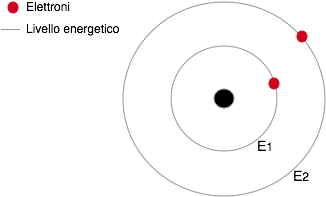
\includegraphics[scale=0.7]{cap1/atomico2liv}
    \caption{Sistema atomico composto da due livelli}
    \label{atomico2liv}
  \end{center}
\end{figure}

Quando la luce investe un materiale, si possono verificare due differenti tipi di transizione:
\begin{itemize}
	\item \emph{Assorbimento}: Quando il fascio di luce investe un materiale, parte dell'energia posseduta dal fascio viene ceduta. L'assorbimento consiste nel cedere, da parte del fotone, la propria energia al sistema atomico permettendo ad un singolo elettrone di passare da uno stato fondamentale $E_{1}$ ad uno stato eccitato $E_{2}$.
	\item \emph{Emissione}: Il sistema atomico cede energia al campo, in questo caso si possono avere due possibili scenari:
	\begin{itemize}
		\item \emph{Spontanea}: L'emissione spontanea si verifica quando un elettrone torna dal livello $E_{2}$ al livello $E_{1}$, provocando l'emissione di un fotone, senza nessun campo di radiazione incidente su di esso. Essa viene definita anche emissione incoerente: l'energia viene emessa con fase e direzione casuale.
		\item \emph{Stimolata}: L'emissione stimolata, invece, si ottiene quando un fotone incidente causa la discesa di un elettrone dal livello $E_{2}$ al livello $E_{1}$ ottenendo così due fotoni alla stessa frequenza. Quindi, in breve, un fotone colpisce l'atomo e due fotoni lo lasciano. Essa viene definita anche emissione coerente: l'energia viene emessa con la stessa fase, frequenza e direzione.
	\end{itemize} 
\end{itemize}
\begin{figure}[H]
  \begin{center}
    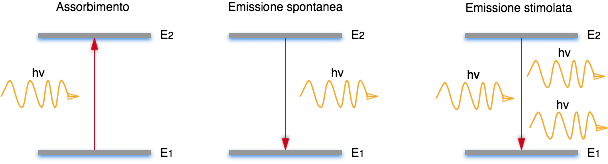
\includegraphics[scale=0.6]{cap1/funzatomoecc}
    \caption{Schema di funzionamento di un atomo eccitato: assorbimento, emissione spontanea ed emissione stimolata}
    \label{funzatomoecc}
  \end{center}
\end{figure}
L'importanza dell'emissione stimolata sta nel fatto che essendo prodotti due fotoni iso-frequenziali, di fatto avviene un'amplificazione ottica, la quale consente il funzionamento del sistema laser.

Per comprendere i meccanismi che regolano lo scambio di energia tra la radiazione ed il sistema atomico, è necessario introdurre la statistica di Boltzmann~\cite{kasap2012optoelectronics}. Attraverso tale statistica \'e possibile definire la popolazione, in termini di densit\'a, di un livello energetico all'equilibrio termico mediante la seguente relazione:
\begin{equation}
  N=N_0e^{{-\frac{E}{kT}}}
\end{equation}
dove $N_0$ \'e la popolazione iniziale in un dato livello energetico e $k=1.38\cdot10^{-23}\frac{J}{K}$\'e la costante di Boltzmann.
 
 Indicando, quindi, con $N_1$ e $N_2$ il numero di atomi per unit\'a di volume (popolazione atomica) per i rispettivi livelli $E_1$ e $E_2$, possiamo ricavare il rapporto tra il numero di atomi nello stato fondamentale e quello nello stato eccitato, all'equilibrio termodinamico alla temperatura $T$, tramite la seguente equazione:
\begin{equation}
	\frac{N_2}{N_1}=e^{-\frac{\Delta E}{kT}} 
	\label{rappboltz}
\end{equation}
dove $\Delta E = E_2 - E_1$.

La condizione necessaria per avere emissione stimolata \'e l'inversione di popolazione tra i due livelli energetici, ovvero, il numero di atomi presenti nel livello eccitato deve essere maggiore di quello fondamentale ($N_2 > N_1$).

In un sistema a due livelli questa condizione non \'e realizzabile poich\'e, come possiamo osservare dall'equazione \ref{rappboltz} a causa della presenza dell'esponenziale negativo, $N_1$ risulta sempre maggiore di $N_2$, ovvero gli atomi a energia minima sono maggiori rispetto a quelli eccitati. 
\'E evidente dunque che, per avere una maggior probabilit\'a di emissione rispetto all'assorbimento, sia necessaria un'inversione di popolazione, ovvero $N_2 > N_1$.

Per ottenere la condizione di inversione di popolazione \'e quindi necessario l'utilizzo di un sistema atomico con almeno tre livelli energetici.

\subsection{Inversione di popolazione}
\begin{figure}[H]
  \begin{center}
    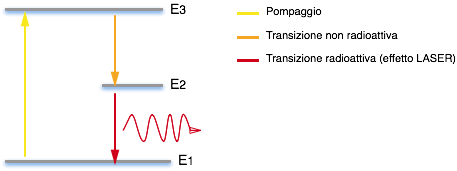
\includegraphics[scale=0.6]{cap1/sistema3liv}
    \caption{Sistema atomico a tre livelli energetici}
    \label{sistema3liv}
  \end{center}
\end{figure}
L'idea di base dell'inversione di popolazione consiste nello sfruttare i diversi tempi di vita medi dei differenti stati energetici.

Considerando un sistema ad esattamente tre livelli energetici ($E_1$, $E_2$ e $E_3$) schematizzato in Figura \ref{sistema3liv}, si sottopone il sistema atomico ad una radiazione luminosa di frequenza $\nu_{31}$, corrispondente al gap energetico $E_3-E_1$, in modo tale che gli elettroni dallo stato $E_1$ si eccitino raggiungendo lo stato instabile $E_3$. Questa prima fase è chiamata \emph{pompaggio}.

Successivamente si manifesta un decadimento dallo stato instabile $E_3$ allo stato $E_2$ in tempi molto rapidi e privi di emissione spontanea. Solitamente l'energia rilasciata viene trasferita sotto forma di moto vibrazionale al materiale circostante e non come fotone emesso.

Dal livello $E_2$ si verifica l'emissione laser alla frequenza $\nu_{21}$ e la conseguente regressione dal livello $E_2$ al livello $E_1$. La condizione necessaria, sui tempi di vita medi, per il funzionamento del laser è $\tau_{32} \ll \tau_{21}$, ovvero che il decadimento da $E_3$ a $E_2$ sia pi\'u rapido di quello da $E_2$ a $E_1$. Tale condizione permette di avere inversione di popolazione, ovvero $N_2 > N_1$, cos\'i da poter innescare l'amplificazione ottica e, quindi, l'effetto laser alla frequenza $\nu_{21}$.

Questo metodo \'e inefficiente perch\'e richiede un pompaggio elevato: \'e necessario fornire un numero elevato di elettroni al livello $E_3$ in modo tale che possa donarli al livello $E_2$ permettendo cos\'i l'inversione di popolazione.

Un struttura pi\'u efficiente \'e quella a quattro livelli schematizzata in Figura \ref{sistema4liv}. In questa disposizione, il pompaggio degli elettroni avviene da $E_1$ a $E_4$ a cui segue una transizione rapida e senza radiazione verso $E_3$ che consente di popolare il livello energetico. A questo punto avviene la transizione lenta e l'emissione tramite azione laser. Infine avviene una rapida transizione da $E_2$ allo stato fondamentale $E_1$.

\begin{figure}[H]
	\begin{center}
		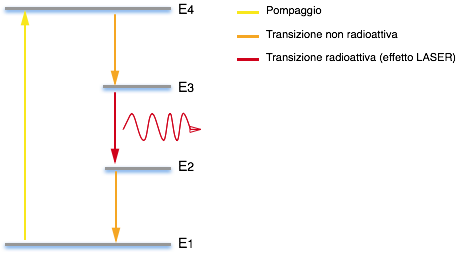
\includegraphics[scale=0.6]{cap1/sistema4liv}
		\caption{Sistema atomico a quattro livelli energetici}
		\label{sistema4liv}
	\end{center}
\end{figure}

A differenza della struttura a tre livelli, questa ha il vantaggio di avere il livello $E_3$ popolato mentre il livello $E_2$ vuoto ($N_2=0$), in quanto gli elettroni decadono rapidamente dallo stato $E_2$ allo stato $E_1$, aiutando a conservare l'inversione di popolazione $N_3 \gg N_2$. 
				
Oltre al meccanismo appena descritto, altre caratteristiche risultano cruciali nel funzionamento del laser: la cavit\'a ottica e il materiale attivo.

\subsection{Cavit\'a ottica e materiale attivo}
Nel paragrafo precedente abbiamo visto come realizzare un materiale amplificatore, che sfrutta l'inversione di popolazione nei livelli energetici. Per generare il fascio laser \'e necessario, per\'o, inserire il materiale attivo all'interno di una cavit\'a ottica.
Una semplice cavit\'a ottica può essere rappresentata dalla cavit\'a a specchi piani e paralleli, nota anche come cavit\'a di Fabry-Perot, mostrata in Figura \ref{cavitaottica}. 
\begin{figure}[H]
	\begin{center}
		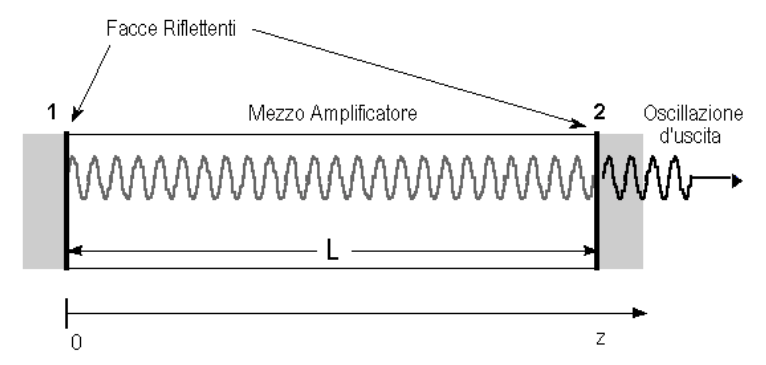
\includegraphics[scale=0.4]{cap1/cavitaottica}
		\caption{Cavit\'a di Fabry-Perot}
		\label{cavitaottica}
	\end{center}
\end{figure}
\begin{figure}[H]
  \begin{center}
    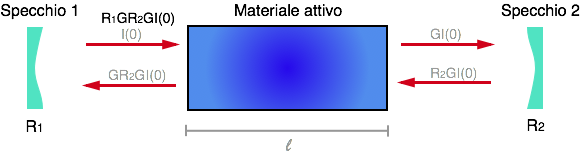
\includegraphics[scale=0.6]{cap1/roundtrip}
    \caption{Schema del Roundtrip ottico nella cavit\'a ottica}
    \label{roundtrip}
  \end{center}
\end{figure}
Il fascio di luce viaggia avanti-indietro riflettendosi negli specchi e amplificandosi nel passaggio all'interno del materiale attivo. Il fascio laser in uscita si ottiene rendendo uno dei due specchi della cavit\'a ottica parzialmente trasparente, in modo tale che parte della radiazione esca dalla cavit\'a.

Per definire il guadagno ottico del materiale attivo \'e necessario introdurre per\'o alcuni concetti preliminari. Indicando con $I$ l'intensità luminosa, definiamo l'intensità della luce all'interno della cavit\'a ottica con la seguente relazione:
\begin{equation}
I(l)=I(0)e^{\sigma(N_2-N_1)l}
\end{equation}
dove $\sigma$ \'e la la \textit{cross section} di emissione e $l$ \'e la lunghezza della cavit\'a ottica.

\begin{figure}[H]
  \begin{center}
    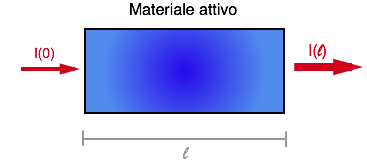
\includegraphics[scale=0.6]{cap1/propagazione}
    \caption{Propagazione della radiazione all'interno della cavità laser}
    \label{propagazione}
  \end{center}
\end{figure}
Possiamo definire il guadagno ottico del mezzo attivo come:
\begin{equation}
  G=\frac{I(l)}{I(0)}=e^{\sigma(N_2-N_1)l}
\end{equation}
sulla quale graveranno le limitazioni dovute alle perdite del materiale e alla perdita utile di potenza dovuta al laser uscente.

La cavità ottica e il mezzo attivo formano quindi un oscillatore ottico, ossia un amplificatore che viene retro-azionato positivamente attraverso specchi riflettenti posti ai lati del materiale attivo. Quindi, per avere un'azione laser è necessario raggiungere una situazione in cui il guadagno di amplificazione sia tale da compensare tutte le perdite presenti. 

Considerando come perdite solamente la riflettività parziale degli specchi $R_1$ e $R_2$, l'oscillazione ottica si innesca quando il guadagno del materiale attivo supera le perdite della cavità in un giro completo, o \textit{round trip}:
\begin{equation}
  G^2=\frac{1}{R_1R_2}
\end{equation}
Quest'ultimo è chiamato guadagno critico o inversione critica.

\section{Laser a semiconduttore}
Un dispositivo laser a semiconduttore utilizza una giunzione p-n come materiale attivo all'interno della cavità ottica. Il pompaggio avviene tramite la ricombinazione di elettroni e lacune, che produce fotoni ad una lunghezza d'onda dipendente dal \textit{gap} tra i livelli energetici del dispositivo: la frequenza della radiazione emessa è legata quindi al tipo di materiali impiegati~\cite{sveltolaser}.

In commercio esistono diverse tipologie di laser a semiconduttore. Esse differiscono sulla base di due aspetti fondamentali: il tipo di cavità ottica impiegata e la forma degli specchi semi-riflettenti necessari a realizzare la retroazione ottica. 

Sulla base di queste due caratteristiche si possono individuare tre categorie principali di laser:
\begin{enumerate}
	\item Laser Fabry-perot
	\item Laser DFB
	\item Laser VCSEL
\end{enumerate}

\subsection{Laser Fabry-Perot}
\begin{figure}[H]
  \begin{center}
    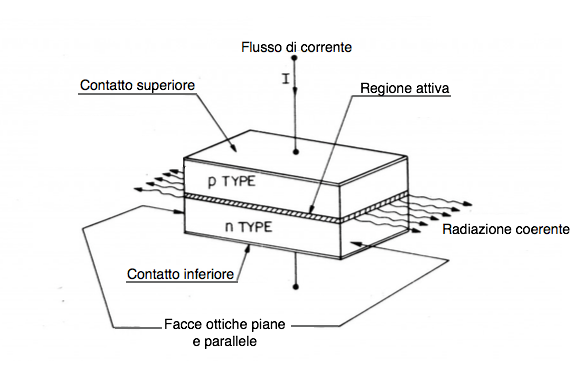
\includegraphics[scale=0.5]{cap1/fabryperot}
    \caption{Laser Fabry-Perot}
    \label{fabryperot}
  \end{center}
\end{figure}
I laser Fabry-Perot hanno la classica configurazione con cavità orizzontale a specchi piani, come mostrato in Figura \ref{fabryperot}.

Il principio di funzionamento é analogo a quello di un oscillatore ottico, descritto per esteso nel paragrafo precedente.

In particolare, la luce presente in cavità stimola alcuni atomi, già eccitati dalla corrente di pompa, ad emettere un fotone isofrequenziale con stessa fase di quello incidente.  
Gli specchi agli estremi della cavità rendono possibile la retroazione positiva, infatti fanno in modo che si possano instaurare alcuni modi di oscillazione stabili, o talvolta solo uno. 

Questo può rappresentare uno svantaggio in applicazioni come l'interferometria.

\subsection{Laser DFB}
\begin{figure}[H]
	\begin{center}
		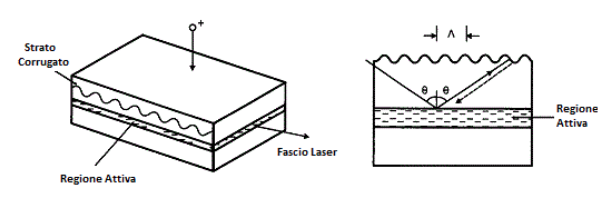
\includegraphics[scale=0.5]{cap1/dfb}
		\caption{Laser DFB}
		\label{dfb}
	\end{center}
\end{figure}
DFB è l'acronimo di \emph{Distributed Feedback Laser}. Il principio di funzionamento è simile a quello dei laser Fabry-Perot, ma con la importante differenza che non sono presenti due specchi separati a formare la cavità ottica ma è inserito uno strato corrugato adiacente allo strato attivo.

Questo strato aggiuntivo è fabbricato in maniera tale da riflettere solo una banda stretta di lunghezze d'onda, così da garantire un singolo modo longitudinale. 

Per questa caratteristica i laser DFB, sono più stabili dei Fabry-Perot, e più adatti ad applicazioni connesse alle fibre ottiche.

\subsection{Laser VCSEL}
\begin{figure}[H]
  \begin{center}
    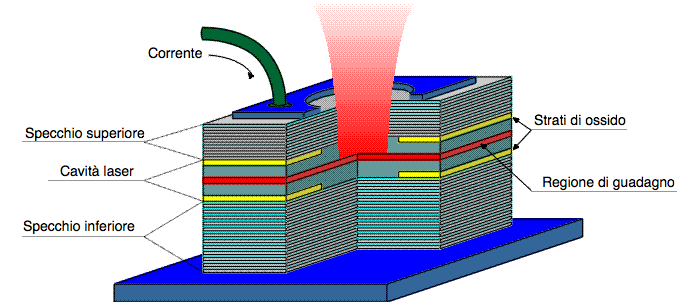
\includegraphics[scale=0.45]{cap1/vcsel}
    \caption{Laser VCSEL}
    \label{vcsel}
  \end{center}
\end{figure}
VCSEL è l'acronimo di \emph{Vertical Cavity Surface-Emitting Laser}. Questi dispositivi, a differenza delle precedenti due categorie, presentano una cavità ottica verticale. 

La cavità ottica ha una lunghezza molto inferiore alle dimensioni laterali del dispositivo, ciò implica che la luce del fascio laser viene emessa dalla superficie piuttosto che dai bordi laterali. 

Poiché la cavità risulta essere più ridotta rispetto alle altre tipologie, a parità di guadagno $G$ occorre aumentare la riflettività degli specchi per ottenere un guadagno d'anello maggiore di uno. A sfavore vi è una limitazione in potenza di emissione dovuta agli specchi altamente riflettenti.

\section{Classi di sicurezza dei laser}
Durante lo sviluppo di un sistema che include l'utilizzo di sorgenti laser è di fondamentale importanza garantire lo svolgimento del lavoro in sicurezza. Infatti, avendo a che fare con sorgenti laser, è importante conoscere i danni che esse possono provocare a cose e persone. In particolare, nei casi più gravi, le sorgenti laser possono procurare danni alla retina dell'occhio e ustioni alla pelle. 

Per poter scegliere in modo appropriato il laser da impiegare nel dispositivo è indispensabile conoscere le norme legislative che ne regolano l'utilizzo~\cite{ans}. A livello europeo vige la normativa \emph{IEC/EN 60825-1} che fissa una classificazione dei fasci laser in funzione della lunghezza d'onda e della potenza ottica emessa. 

La suddetta normativa classifica la pericolosità di una sorgente laser suddividendola in 4 classi:
\begin{itemize}
	\item \emph{Classe 1}: Questa classe include le sorgenti laser che non arrecano danni a cose e/o persone
	\item \emph{Classe 2}: Questa classe comprende i laser che emettono nell'intervallo di lunghezza d'onda compreso tra $400nm$ e $700nm$. Possono provocare danni alla retina dell'occhio in caso di osservazione prolungata.
	\item \emph{Classe 3}: Questa classe comprende due sotto-classi.
		\begin{itemize}
		\item \emph{Classe 3A}: Questa classe include tutte le sorgenti laser che risultano sicure per una visione naturale e non mediante strumenti ottici (es. microscopi)
		\item \emph{Classe 3B}: Questa classe include tutte le sorgenti laser che risultano pericolose per una visione naturale. \'E necessario utilizzare protezioni per gli occhi e disporre delle segnalazioni di avvertimento nella zona in cui si utilizza il laser. 
		\end{itemize}
	\item \emph{Classe 4}: Questa classe include le sorgenti laser più pericolose. Possono causare lesioni alla pelle e costituiscono pericolo d'incendio. 
\end{itemize}
\begin{figure}[H] 
  \begin{center}
    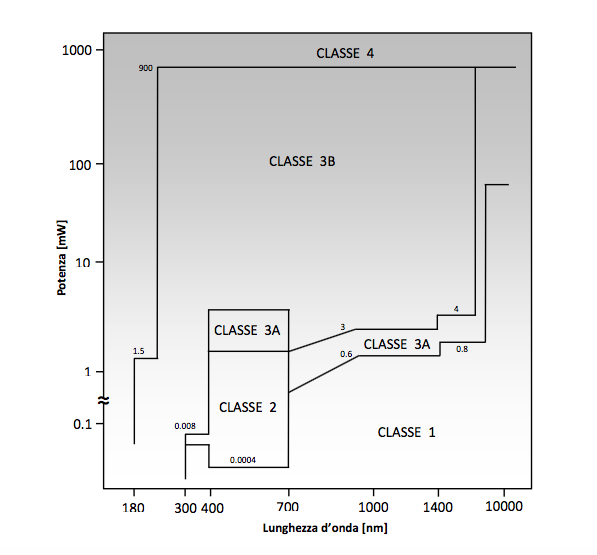
\includegraphics[scale=0.5]{cap1/classisicurezza}
    \caption{Classi di sicurezza dei laser}
    \label{classisicurezza}
  \end{center}
\end{figure}
La classificazione appena descritta è rappresentata in Figura \ref{classisicurezza}, insieme alle lunghezza d'onda corrispondenti a ciascuna classe.

\section{Telemetri ottici}
La telemetria è un insieme di metodi di osservazione aventi lo scopo di fornire la misura della distanza di un oggetto dall'osservatore.

Lo strumento che effettua la misura è chiamato telemetro: esso rileva la distanza assoluta tra lo strumento stesso e un oggetto remoto, chiamato bersaglio. In commercio esistono diverse tipologie di telemetri che si basano sull'impiego di sorgenti laser.

Le tipologie più diffuse sono tre: 
\begin{enumerate}
	\item A triangolazione
	\item A tempo di volo
	\item A onda continua
\end{enumerate}

\subsection{Telemetri a triangolazione}
\begin{figure}[H]
  \begin{center}
    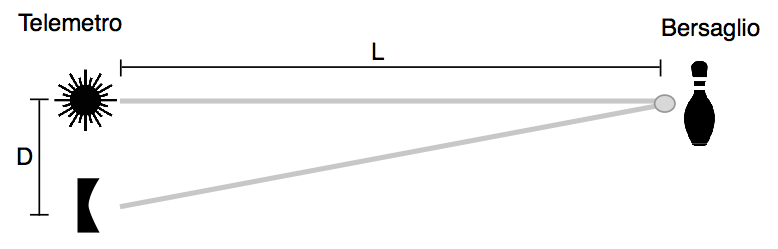
\includegraphics[scale=0.5]{cap1/triangolazione}
    \caption{Schema di funzionamento di un telemetro a triangolazione}
    \label{triangolazione}
  \end{center}
\end{figure}
I telemetri a triangolazione utilizzano una sorgente laser e un'ottica di ricezione posti perpendicolarmente ad una distanza $D$ tra loro. Inoltre, la sorgente laser è posizionata ad una distanza $L$ dal bersaglio. Si dice, quindi, che il bersaglio è "triangolato" da due punti a distanza $D$ su una stessa linea di base. Lo schema è mostrato in Figura \ref{triangolazione}.

Questo tipo di telemetro si basa sul principio della triangolazione, quindi valuta la distanza del bersaglio, conoscendo l'angolo $\alpha$ con cui il fascio laser viene riflesso sull'ottica di ricezione. 

Tramite questo angolo, infatti, è possibile ricavare la seguente relazione:
\begin{equation}
	\frac{D}{L}=\tan\alpha\approx\alpha
\end{equation}
Questa approssimazione è valida solo se $\alpha \ll 1$. 

L'angolo $\alpha$ si trova valutando la posizione in cui il fascio colpisce il fotorivelatore, secondo la relazione: 
\begin{equation}
  \alpha=\frac{x}{f_{rec}}
\end{equation}
dove $x$ è la distanza del punto di incidenza sul fotorivelatore dall'asse ottico della lente di ricezione, mentre $f_{rec}$ è la lunghezza focale dell'ottica di ricezione.

La misura della distanza si ricava facilmente dalle precedenti relazioni:
\begin{equation}
  L=\frac{D}{x}f_{rec}
\end{equation}
Differenziando quest'ultima equazione si trova l'errore di misura assoluto $\Delta L$ dovuto al minimo spostamento misurabile $\Delta x$ sul rivelatore: 
\begin{equation}
	 \Delta L=-\frac{D}{x^2}f_{rec}\Delta x
\end{equation}
Ricavando quindi un errore di misura relativo pari a:
\begin{equation}
\frac{\Delta L}{L}=-\frac{\Delta x}{x}=-\frac{\Delta\alpha}{\alpha}
\end{equation}
Il principale svantaggio di questa tecnica è che, con l'aumentare della distanza $L$, l'angolo $\alpha$ diminuisce, e ciò comporta l'aumento dell'incertezza relativa $-\frac{\Delta\alpha}{\alpha}$.
 
Per tale motivo, questa tipologia di telemetro è utilizzata per la misura di brevi distanze ($0.1\div 10 m$) .

\subsection{Telemetri a tempo di volo}
\begin{figure}[H]
	\begin{center}
		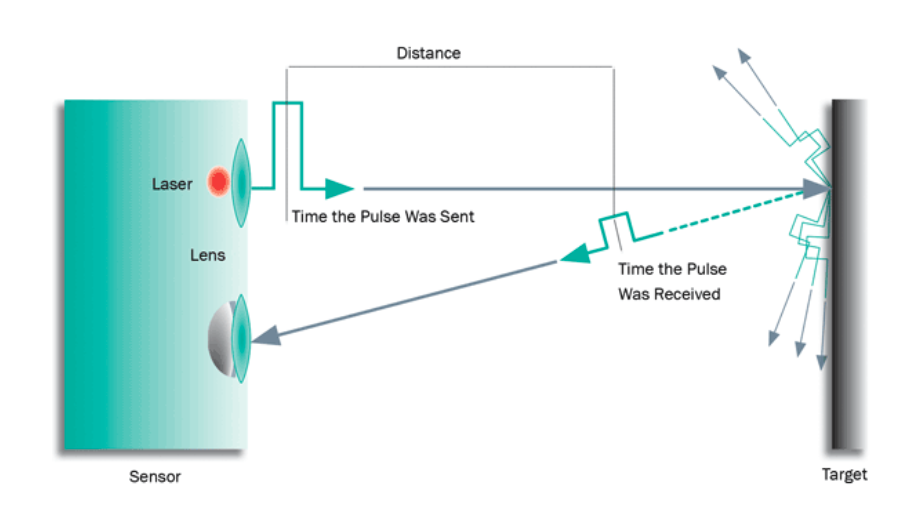
\includegraphics[scale=0.4]{cap1/tempodivolo}
		\caption{Schema di funzionamento di un telemetri a tempo di volo}
		\label{tempodivolo}
	\end{center}
\end{figure}
I telemetri a tempo di volo utilizzano un laser impulsato. Essi emettono potenza solo per un brevissimo istante di tempo $\tau$.

Con un bersaglio posto a distanza $L$ dalla sorgente laser, il fascio laser percorre un cammino pari a $2L$ (Andata e Ritorno) in un tempo $T$ viaggiando a velocità della luce $c\approx3\cdot10^8\frac{m}{s}$, ricavando così la seguente relazione:
\begin{equation}
  L=\frac{c}{2}T
\end{equation}
Differenziando la precedente equazione si ottiene:
\begin{equation}
  \Delta L=\frac{c}{2}\Delta T
\end{equation}
\begin{equation}
  \frac{\Delta L}{L}=\frac{\Delta T}{T}
\end{equation}
Si può osservare come la misura $\Delta L$ dipenda unicamente dal $\Delta T$ che si riesce a risolvere. In pratica, la misura viene effettuata utilizzando un contatore che conta quanti tempi di clock $\Delta T$ sono intercorsi tra l'istante di partenza del raggio laser e il momento in cui ritorna all'ottica di rivelazione.

Il vincolo di questi telemetri è che la durata dell'impulso $\tau$ deve soddisfare la condizione $\tau \ll \Delta T$. Per tale motivo sono utilizzati per misure di distanze medio-lunghe (fino a $10 Km$). 

\subsection{Telemetri a onda continua}
\begin{figure}[H]
  \begin{center}
    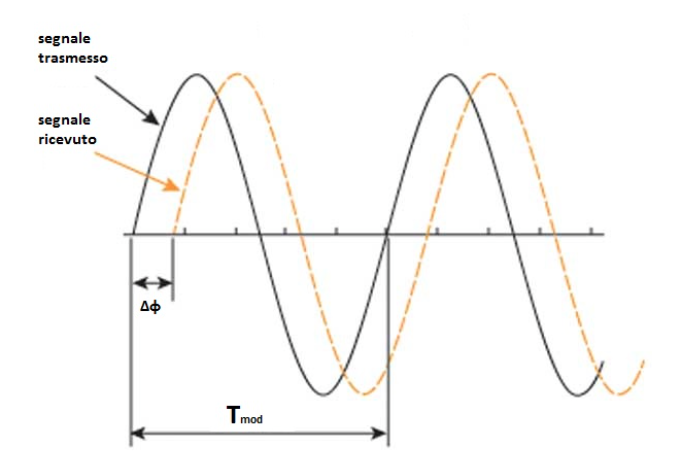
\includegraphics[scale=0.4]{cap1/ondacontinua}
    \caption{Potenza trasmessa e potenza riflessa in un telemetro a onda continua}
    \label{ondacontinua}
  \end{center}
\end{figure}
I telemetri a onda continua hanno un funzionamento analogo ai telemetri a tempo di volo, ma a differenza di questi ultimi, la potenza ottica viene modulata sinusoidalmente a frequenza $f_{mod}$ ottenendo il segnale in Figura \ref{ondacontinua}.

La potenza trasmessa dal laser vale quindi:
\begin{equation}
	 P(t)=P_0[1+msin(2\pi f_{mod}t)]
\end{equation} 
Nella pratica, la misura non viene effettuata con un contatore elettronico, come per i telemetri a tempo di volo, ma avviene mediante la rilevazione del ritardo di fase $\Delta\phi$ tra il segnale ricevuto $P_r$ e il segnale trasmesso $P_t$.

Considerando la relazione:
\begin{equation}
  \frac{\Delta\phi}{2\pi}=\frac{\Delta t}{T_{mod}}
\end{equation}
dove $\Delta t=\frac{2L}{c}$ e $T_{mod}=\frac{1}{f_{mod}}$, si ottiene così la misura di distanza assoluta:
\begin{equation}
  L=\frac{c}{2}\frac{1}{2\pi f_{mod}}\Delta\phi=\frac{\Delta\phi}{S}
\end{equation}
Dall'ultima equazione si può notare come la sensibilità $S$ della misura migliori all'aumentare della frequenza di modulazione. Tuttavia un aumento eccessivo della frequenza di modulazione comporta una riduzione della massima distanza rilevabile. 

Questo tipo di telemetro si utilizza per misure comprese tra $1$ e $1000m$, con risoluzioni dell'ordine del millimetro. 

\section{Una tecnica alternativa per la misura}
Come già discusso nell'Introduzione, lo scopo di questo lavoro di Tesi è realizzare il prototipo di un misuratore di distanza assoluta che sia a basso costo e con ingombro limitato per poter essere più maneggevole nella misura di medio-brevi distanze.

Da quanto esposto nel precedente paragrafo, emerge che i telemetri descritti non sono i'n grado di raggiungere tali obiettivi. Infatti tali strumenti sono adatti per la misura di distanze dell'ordine della decina di metri. Per quanto riguarda i telemetri a triangolazione, invece, esistono in commercio strumenti in grado di misurare distanze brevi con buona sensibilità. Tuttavia questi dispositivi, oltre ad avere un costo elevato, necessitano di un'ottica specifica per la ricezione della radiazione riflessa e di un bersaglio cooperativo.

Da queste osservazioni si conclude che, per raggiungere l'obiettivo preposto, è necessario utilizzare una tecnica di misura che si differenzia da quelle comuni, ovvero l'\textbf{interferometria a retroiniezione}. Questa tecnica verrà ampiamente discussa nel Capitolo \ref{capitolo2}.











 








\chapter{Interferometria a retroiniezione}
\label{capitolo2}
\thispagestyle{empty}

\textit{In questo Capitolo verranno trattati i principi di base dell'interferometria, in particolare verrà presentata la tecnica utilizzata dello strumento di misura sviluppato in questo lavoro di Tesi: l'interferometria a retroiniezione. Dopo aver descritto il principio di funzionamento dell'interferometria a retroiniezione, saranno esposti i principali vantaggi, svantaggi e limitazioni di questa tecnica. In conclusione, verranno descritti i campi di applicazione della tecnica a retroiniezione ponendo particolare attenzione al campo d'applicazione dello strumento sviluppato: la misura di distanza assoluta.}

\section{Principi di interferometria convenzionale}
L'interferometria convenzionale è una tecnica che si basa sulla sovrapposizione di due o più fasci ottici, emessi dalla stessa sorgente, al fine di ottenere una frequenza di battimento (frequenza risultante dalla sovrapposizione) che contiene informazioni sui differenti cammini percorsi dai due fasci. Questa tecnica è in accordo con la teoria ondulatoria della luce che attribuisce alla propagazione della luce le caratteristiche della propagazione delle onde (elettromagnetiche) elastiche. Essa si basa sul fenomeno dell'interferenza e in particolare si sfrutta il principio secondo cui un'onda risultante dalla combinazione di due onde differenti mantiene proprietà che dipendono dalle onde generatrici.

I campi di applicazione di tale tecnica spaziano dall'astronomia alla metrologia ottica. Essa, in generale, trova applicazioni in ambiti dove l'ambiente di lavoro è critico (ad esempio superfici calde) o l'oggetto da misurare è difficilmente raggiungibile.
\begin{figure}  
  \begin{center}
    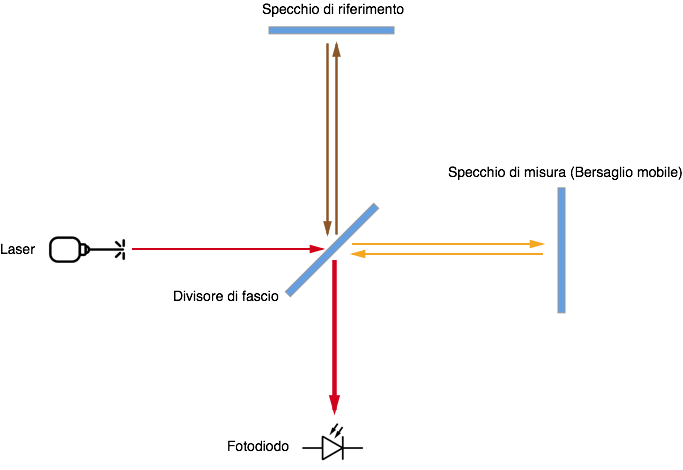
\includegraphics[scale=0.4]{cap2/michelson}
    \caption{Interferometro di \textit{Michelson}}
    \label{michelson}
  \end{center}
\end{figure}
La configurazione ottica interferometrica classica, mostrata in Figura \ref{michelson}, è definita interferometro di \textit{Michelson}~\cite{sensmeslaser}. Questa configurazione è costituita da una sorgente laser, un divisore di fascio (\textit{beam splitter}), due specchi e un fotodiodo.

Il funzionamento dell'interferometro di \textit{Michelson} consiste nel duplicare il fascio ottico emesso dalla sorgente laser, tramite uno specchio semiriflettente (divisore di fascio), in due cammini ottici distinti, di cui uno noto (di riferimento) e uno di misura. Entrambi i fasci, vengono riflessi da due specchi posti all'estremità dei due cammini. Lo specchio posto nel ramo di riferimento è fisso, mentre quello posto sul ramo di misura è mobile. Successivamente i fasci di riferimento e di misura vengono sovrapposti e indirizzati, attraverso il \textit{beam splitter}, verso il fotodiodo. Il fascio risultante è la combinazione di due fasci iso-frequenziali, ma sfasati a causa dei diversi cammini percorsi.

Infine, il fotodiodo produce una corrente, proporzionale all'intensitá del fascio laser incidente su di esso, che contiene l'informazione sullo spostamento del bersaglio. Tale corrente fotogenerata è associata alla potenza incidente che è proporzionale alla somma dei campi elettrici dei rispettivi cammini.

Indicando con ${E_m}$ il campo elettrico relativo al cammino di misura e con ${E_r}$ il campo elettrico relativo al cammino di riferimento, la corrente fotogenerata $I_{ph}$ segue la relazione:
\begin{equation}
\begin{split}
	I_{ph}&=\sigma|E_r+E_m|^2=\sigma\{E_r^2+E_m^2+2E_rE_mRe[e^{i(\phi_m-\phi_r)}]\}\\
	&=I_r+I_m+2\sqrt{I_rI_m}\cos{(\phi_m-\phi_r)}
\end{split}
\end{equation}
dove $\sigma$ è il coefficiente di conversione del fotodiodo, $E_r$ e $E_m$ sono rappresentati come vettori rotanti di ampiezza $|E_{m,r}|$ e fase $\phi_{m,r}$ e la terza componente $2\sqrt{I_rI_m}\cos{(\phi_m-\phi_r)}$ costituisce la fase interferometrica. 

Per come é costruito l'interferometro di \textit{Michelson}, si avrà che la fase $\phi_r$ sará sempre costante, mentre quella relativa a $\phi_m$ varierá in funzione dello spostamento dell'ostacolo. Quindi ció che si ottiene sará una corrente fotogenerata che dipenderá dal coseno della fase $\phi_m$. 

Indicando con $k=\frac{2\pi}{\lambda}$ il numero d'onda (numero di oscillazione nell'unità di lunghezza) è possibile esplicitare l'argomento del coseno ottenendo:
\begin{equation}
	\phi=ks=\frac{2\pi}{\lambda}s	
\end{equation}
dove $\lambda$ è la lunghezza d'onda della sorgente laser e $s$ è lo spostamento.

Essendo $\phi_r= ks_r$ e $\phi_m = ks_m$, si può ricavare la variazione di fase totale, ottenendo:
\begin{equation}
	\Delta \phi=\phi_m-\phi_r=k(s_m-s_r)=\frac{2\pi}{\lambda}(s_m-s_r)
\end{equation}
dove $s_m$ e $s_r$ sono rispettivamente i cammini ottici di misura e di riferimento.

La variazione di fase del segnale interferometrico contiene quindi l'informazione sullo spostamento del bersaglio rispetto al cammino di riferimento. Il segnale interferometrico è quindi periodico per sfasamenti totali pari a $2\pi$, che corrispondono ad uno spostamento $s_m$ pari a $\frac{\lambda}{2}$. La misura avviene tramite il semplice conteggio delle frange interferometriche del segnale nel tempo. La risoluzione dello strumento di misura risulta quindi essere pari a  $\frac{\lambda}{2}$.

\subsection{Svantaggi dell'interferometria convenzionale} 
L'interferometro di \textit{Michelson} è molto vantaggioso dal punto di vista della semplicità di realizzazione perché vi è un impiego ridotto di componenti, ma presenta tuttavia notevoli svantaggi nella pratica:
\begin{figure}  
  \begin{center}
    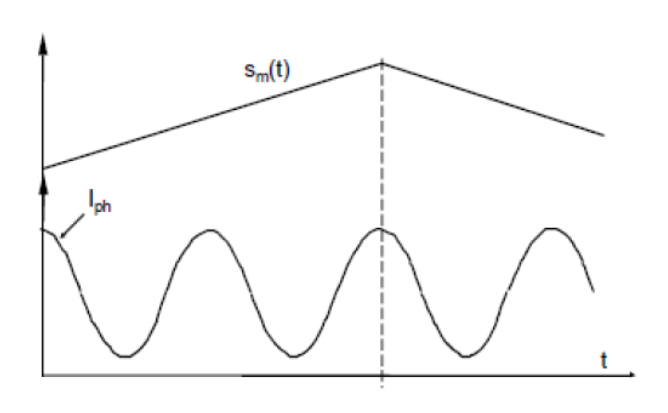
\includegraphics[scale=0.4]{cap2/versospost}
    \caption{Ambiguità sul verso di spostamento}
    \label{versospost}
  \end{center}
\end{figure}
\begin{itemize}
	\item L'allineamento degli specchi, per far convergere i due fasci di luce coerenti nello stesso punto, e il posizionamento del \textit{beam splitter} richiedono accuratezza elevata e sono quindi di difficile realizzazione.
	\item Richiede l'utilizzo di un bersaglio cooperativo e di una particolare ottica di collimazione. Non realizzabile in caso di misura non invasiva.
	\item Non permette di discriminare il verso di spostamento del bersaglio con conseguente ambiguità del movimento misurato. Tale ambiguità è causata dalla risposta cosinusoidale, come mostrato in Figura \ref{versospost}.
	\item La misura subisce alterazioni in caso di retroiniezione non voluta di luce esterna all'interno della cavità ottica del laser.
	\item L'utilizzo di sorgenti laser a gas comporta elevati costi di realizzazione dello strumento.
\end{itemize}
Tutto ciò ha fatto emergere la necessità di uno strumento che presentasse una semplicità di utilizzo e un costo contenuto.

\section{Interferometria a retroiniezione}
È stato esposto, nel paragrafo precedente, come l'interferometria convenzionale presenti notevoli svantaggi. Per tale motivo viene presentata una differente tecnica interferometrica: si tratta dell'interferometria a retroiniezione, chiamata anche interferometria a self-mixing~\cite{1464-4258-4-6-371}.

La tecnica interferometrica a retroiniezione rende possibile la realizzazione di uno strumento di misura tramite il semplice utilizzo di una sorgente laser e di una lente per focalizzare il raggio ottico. Questa configurazione interferometrica risolve, quindi, i problemi dell'interferometria convenzionale, presentando una ridotta complessità di realizzazione e un costo contenuto. Per tale motivo il misuratore realizzato in questo lavoro di tesi sfrutta codesta tecnica.

\begin{figure}  
  \begin{center}
    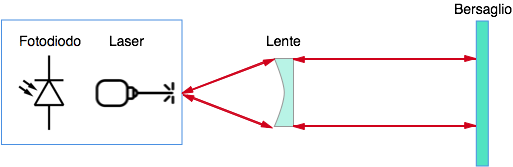
\includegraphics[scale=0.5]{cap2/selfmix}
    \caption{Schema di principio di un interferometro a retroiniezione}
    \label{selfmix}
  \end{center}
\end{figure}

La configurazione base del misuratore a self-mixing è formata da un diodo laser, posto a distanza $s$ dal bersaglio, un'ottica collimatrice e un fotodiodo, che può essere anche quello di monitor integrato nello stesso package del laser. Lo schema base è riportato in Figura \ref{selfmix}.

La modalitá self-mixing, a differenza dell'interferometro convenzionale, non utilizza porzioni di fascio ottico come riferimento. Per effettuare la misura viene sfruttata una porzione di luce riflessa dalla superficie del bersaglio che, rientrando nella cavità laser attraverso la lente, genera un battimento ottico con l'onda laser già presente. La luce riflessa dal bersaglio arriva con verso opposto al precedente cammino e con una potenza che è una frazione di quella emessa, a causa dell'attenuazione data dal tragitto laser-ostacolo-laser.

\'E possibile esplicitare la potenza della luce riflessa dal bersaglio con la relazione:
\begin{equation}
	P_r=\frac{P_0}{A}
\end{equation}
dove $P_0$ è la potenza ottica della radiazione emessa e $A$ è il coefficiente di attenuazione.

All'interno della cavità ottica del laser si verifica un fenomeno di interferenza: il campo elettrico $E_0$ della radiazione emessa si combina con il campo elettrico $E_r$ della luce retroiniettata. Come descritto nel paragrafo precedente, anche in questa situazione, $E_r$ risulta avere uno sfasamento ottico che è pari a:
\begin{equation}
	\phi=2ks
\end{equation}
dove $k=\frac{2\pi}{\lambda}$ è il numero d'onda e $s$ è la distanza.
\begin{figure}  
  \begin{center}
    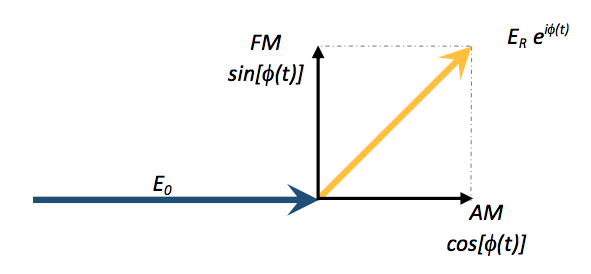
\includegraphics[scale=0.5]{cap2/rapprvet}
    \caption{Rappresentazione vettoriale dell'interferenza all'interno della cavità laser}
    \label{rapprvet}
  \end{center}
\end{figure}
Come mostrato in figura \ref{rapprvet} è possibile scomporre $E_r$, operando un'analisi vettoriale, nelle sue componenti in fase ed in ampiezza. Ciò permette, nella cavità ottica, sia la modulazione in frequenza (FM) che la modulazione in ampiezza (AM) del campo elettrico emesso originariamente dalla sorgente $E_0$. 

La componente che opera la modulazione d'ampiezza è $E_r\cos[\phi(t)]$, mentre la componente di modulazione di frequenza è $E_r\sin[\phi(t)]$. Le' due componenti sono sfasate di $90\degree$ e quindi la discriminazione dei due segnali in quadratura permette di ricavare senza ambiguità il verso dello spostamento del bersaglio, al contrario dell'interferometro di \textit{Michelson}.

L'equazione che governa la corrente nel fotodiodo sará:
\begin{equation}
	I_{ph}=I_0(1+m_{AM})\cos{[(1+m_{FM})\omega t]}
\end{equation}
dove $m_{AM}$ e $m_{FM}$ sono le profondità di modulazione.

Se si utilizza un laser a semiconduttore, come nel caso dello strumento presentato in questa Tesi, la componente FM presente nel fotodiodo é impossibile da estrarre in quanto presenta frequenze dell'ordine delle decine di $MHz$. Quindi, l'unica modulazione visibile sulla corrente del fotodiodo è quella AM:
\begin{equation}
	I_{ph}=I_0(1+m_{AM})\cos{[\omega t]}
\end{equation}
Il funzionamento di un diodo laser a singolo modo longitudinale soggetto a retroiniezione è descritto dalle equazioni differenziali sviluppate da Lang\&Kobayashi~\cite{1070479}; tuttavia, la risoluzione analitica di tali equazioni non è necessaria ai fini di questo lavoro di tesi.

Per questo motivo nel paragrafo successivo è presentata soltanto una soluzione qualitativa delle equazioni di Lang\&Kobayashi, con lo scopo di determinare i regimi di retroiniezione della tecnica self-mixing.

\subsection{Regimi di retroiniezione tramite risoluzione qualitativa}
\begin{figure}  
  \begin{center}
    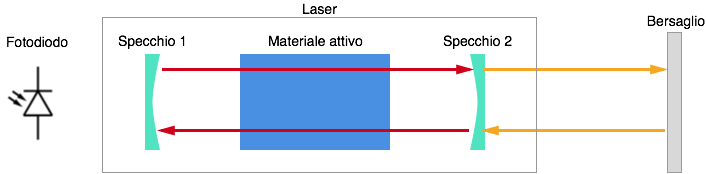
\includegraphics[scale=0.5]{cap2/roundtrips}
    \caption{Round trip ottico del campo elettrico all'interno della cavità laser}
    \label{roundtrips}
  \end{center}
\end{figure}
Un approccio qualitativo per determinare i regimi di retroiniezione è quello di considerare il \textit{round trip} del campo elettrico di Figura \ref{roundtrips}. In figura sono stati evidenziati i \textit{round trip} all'interno della cavità e tra il bersaglio e la cavità stessa.

Il campo elettrico totale presente all'interno della cavità è dato dalla somma di due campi elettrici: quello dovuto alla riflessione dello specchio interno posto al lato opposto della cavità e quello dovuto alla riflessione del bersaglio. Il campo elettrico risultante è quindi:
\begin{equation}
	E'=ER_1R_2e^{2\gamma L}e^{2jkL}+E\alpha e^{2jks}
\end{equation}
dove:
\begin{itemize}
	\item $R_1$ e $R_2$ sono rispettivamente le riflettività dello specchio in cavità e del bersaglio
	\item $\gamma$ è il guadagno netto per unità di lunghezza
	\item $L$ è la lunghezza della cavità
	\item $s$ è la distanza tra il secondo specchio ed il bersaglio
	\item $\alpha$ è il fattore di riflessione (o diffusione) del bersaglio
\end{itemize}

\'E possibile, quindi, ricavare facilmente dall'equazione precedente il guadagno d'anello:
\begin{equation}
	G_{loop}=\frac{E}{E'}=R_1R_2e^{2\gamma L}e^{2jkL}+\alpha e^{2jks}
	\label{gloop}
\end{equation}
Per far si che il sistema sia in grado di produrre oscillazioni spontanee che si mantengano nel tempo con ampiezza costante è necessario rispettare il criterio di \textit{Barkhausen}, il quale afferma che il sistema non deve modificare l'ampiezza del segnale e non deve introdurre sfasamento complessivo. Tali condizioni sono riassunte come segue:
\begin{equation}
	\begin{cases}
   |G_{loop}|=1\\\Phi_{loop} = 0
   \end{cases}
\end{equation}
Per studiare le soluzioni del sistema, si divide l'analisi del problema in due casi:
\begin{enumerate}
	\item In assenza di retroazione 
	\item In presenza di retroazione
\end{enumerate}
Nel primo caso, ovvero con coefficiente $\alpha$ nullo, si trovano le stesse equazioni di un normale laser in cui il guadagno e le perdite sono uguali, ovvero:
\begin{equation}
	\begin{cases}
   G_{loop}=R_1R_2e^{2\gamma L}\\\Phi_{loop} = 2kN=N2\pi
   \end{cases}
   \label{sistnoretr}
\end{equation}
con:
\begin{equation}
k=2\pi n_l \frac{\nu_0}{c}	
\end{equation}
\begin{equation}
	\nu_0 = N\frac{c}{2n_lL}
\end{equation}

dove $k$ è il numero d'onda, $\nu_0$ sono i modi di risonanza e $n_l$ rappresenta l'indice di rifrazione del mezzo attivo.

Se la frequenza reale si discosta da quella di risonanza propria, la frazione di fase $2kL$ in eccesso rispetto ad un multiplo di $2\pi$ può essere scritta come:
\begin{equation}
	2kL=4\pi n_l L \frac{\nu - \nu_0}{c}
\end{equation}

Infatti, in un interferometro con laser Fabry-Perot, la frequenza di risonanza diminuisce all'aumentare della lunghezza $L$ della cavità. Tale affermazione è resa valida dalla relazione differenziale:
\begin{equation}
	\frac{\Delta L}{L} = \frac{\Delta \lambda}{\lambda} = - \frac{\Delta \nu}{\nu}
\end{equation}

Se invece si è in presenza di retroiniezione (secondo caso), ovvero con coefficiente $\alpha$ non nullo, l'equazione \ref{gloop} diventa:
\begin{equation}
	R_1R_2e^{2\gamma L}\sin{ \left (4\pi n_l L \frac{\nu - \nu_0}{c} \right )} + \alpha \sin{(2ks)} = 0
	\label{regimeretr}
\end{equation}

Ipotizziamo il termine di variazione di frequenza $(\nu-\nu_0)$ abbastanza piccolo da poter approssimare $\sin(x)$ con $x$. Mettendo l'equazione \ref{regimeretr} a sistema con le equazioni presenti in \ref{sistnoretr} e considerando l'approssimazione e la sostituzione dei parametri, si ottiene la condizione di risonanza:
\begin{equation}
	2ks=4\pi s \frac{\nu}{c} \approx 4\pi s \frac{\nu_0}{c}
\end{equation}
\begin{equation}
	(\nu - \nu_0) + \left[ \frac{c}{4\pi n_l L}\alpha \sin{\left (\frac{4 \pi s \nu_0}{c}\right )} \right] = 0
\end{equation}

Indicando, infine, con $\nu'=(\nu-\nu_0)$ lo scostamento della frequenza reale rispetto a quella ideale, la modulazione della frequenza vale: 
\begin{equation}
	\nu'= \frac{c}{4\pi n_l L} \alpha \sin \left ( \frac{4 \pi s \nu_0}{c} \right )
\end{equation}

\begin{figure}  
  \begin{center}
    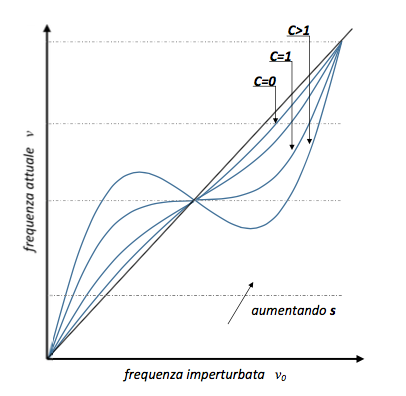
\includegraphics[scale=0.5]{cap2/pertfreq}
    \caption{Perturbazione della frequenza reale rispetto alla frequenza ideale}
    \label{pertfreq}
  \end{center}
\end{figure}

In Figura \ref{pertfreq} è rappresentata la relazione tra la frequenza reale $\nu$ e la frequenza imperturbata $\nu_0$ all'aumentare dello spostamento $s$ del bersaglio. Dalla relazione si ottiene una sinusoide sovrapposta alla bisettrice del primo quadrante periodica di $2\pi$. 

Ogni salto è equivalente a spostamenti $s$ pari a $\frac{\lambda}{2}$, quindi la distanza del bersaglio si puó esprimere come un multiplo intero di $\frac{\lambda}{2}$ sommato allo scarto $\Delta s$:
\begin{equation}
	s= N \frac{\lambda}{2} + \Delta s
\end{equation}
assumendo $\Delta s$ minore di $\frac{\lambda}{2}$.

Le intersezioni tra le linee tratteggiate e le curve sinusoidali, mostrate in Figura \ref{pertfreq}, indicano i punti di lavoro del sistema: spostando il bersaglio della quantità $\delta s$, la frequenza reale assume il valore dato dall'intersezione tra la linea tratteggiata e la curva.

In base all'ampiezza della sinusoide si possono distinguere due regimi di funzionamento:
\begin{enumerate}
	\item \textit{Regime di bassa retroiniezione}
	\item \textit{Regime di alta retroiniezione}
\end{enumerate}

Si dice regime di bassa iniezione quando l'ampiezza della sinusoide sovrapposta è piccola e vi è un unico punto di intersezione che corrisponde alla frequenza reale $\nu$.

Si dice regime di alta iniezione, invece, quando l'ampiezza della sinusoide è grande e vi sono tre o più punti di intersezione rappresentanti la frequenza reale $\nu$. Per distinguere la frequenza effettiva, in regime di alta iniezione, è necessario conoscere le condizioni del laser prima dello spostamento $\Delta s$~\cite{randonethesis}.

Il limite tra i due regimi sta nel punto centrale del grafico in cui vi è un flesso a tangente orizzontale. Tale condizione può essere espressa matematicamente con il sistema:
\begin{equation}
	\begin{cases}
   \frac{d(y=x+Asin(Bx))}{dx}=0\\Bx=\pi
   \end{cases}
   \label{sistflesso}
\end{equation}
dove $A=- \frac{c}{4 \pi n_l L}\alpha$ e $B=\frac{4\pi s}{c}$. Dal sistema \ref{sistflesso} si ricava $AB=1$ e sostituendo i parametri fisici si ottiene:
\begin{equation}
	\frac{c}{4 \pi n_l L} \alpha \frac{4\pi s}{c} = \frac{\alpha s}{n_l L} = 1
\end{equation}

Arrivati a questo punto si è in grado di definire il fattore $C$ come indice della retroiniezione del sistema interferometrico a self-mixing:
\begin{equation}
	C = \frac{\alpha s}{n_l L}
\end{equation}

Nel caso in cui la sorgente laser considerata utilizzi come materiale attivo un semiconduttore, il parametro $C$ diventa:
\begin{equation}
	C=\alpha s \frac{\sqrt{1+\alpha_{en}^2}}{n_l L}
\end{equation}
dove $\alpha_{en}$ è il fattore di allargamento di riga che tipicamente assume valori tra $2$ e $6$ nel caso di laser a stato solido.

Come descritto in precedenza non verrà trattata la risoluzione matematica delle equazioni di Lang\&Kobayashi, ma si analizzeranno solo i risultati. Per una trattazione completa si faccia riferimento alla letteratura~\cite{1070479}.

Risolvendo le equazioni di Lang\&Kobayashi si ottiene che con lo spostamento del bersaglio, non è modulata unicamente la frequenza propria di oscillazione del laser, ma anche la potenza ottica emessa dal laser, che in condizioni di retroazione è pari a:
\begin{equation}
	P(\Phi)=P_0(1+mF(\Phi))
\end{equation}
dove:
\begin{itemize}
	\item $P_0$ è la potenza emessa del laser in assenza di retroiniezione 
	\item $m$ rappresenta l'ampiezza del segnale a frange sovrapposto al termine costante (profondità di modulazione)
	\item $\Phi = 2ks$ è lo sfasamento tra l'onda emessa e quella retroiniettata 
	\item $F(\Phi)$ è una funzione di periodo $2\pi$ che assume valori di ampiezza compresi tra $-1$ e $+1$:
		\begin{equation}
			F(\Phi(t))=F(2ks(t))=F(2\frac{2\pi}{\lambda}s(t))
		\end{equation}
\end{itemize}

L'andamento della funzione $F(\Phi)$ è influenzato dal fattore $C$. La conseguenza è che $F(\Phi)$  dipende da 3 fattori:
\begin{enumerate}
	\item distanza del bersaglio
	\item riflettività del bersaglio 
	\item parametri del laser
\end{enumerate}
Si possono, quindi, identificare quattro possibili regimi di funzionamento per un interferometro a self-mixing sulla base del parametro $C$:
\begin{enumerate}
	\item \textit{Regime di retroiniezione molto debole} ($0 < C \leq 0.1$): la quantità di potenza ottica che rientra in cavità è molto ridotta a causa di un'elevata riflettività degli specchi o di bassi coefficienti di riflessione della superficie del bersaglio. La funzione $F(\Phi)$ è un coseno di ampiezza molto ridotta, tipicamente $10^{-4}$ rispetto al valore in continua.
	\item \textit{Regime di retroiniezione debole} ($0.1 < C < 1$): La funzione $F(\Phi)$ inizia a distorcersi e non è più simmetrica. La maggior parte dei casi pratici rientra in questo regime di funzionamento. 
	\item \textit{Regime di retroiniezione moderata} ($1 < C \leq 4.6$): Per i valori di $C$ presenti in questo intervallo ci sono tre punti di intersezione in Figura \ref{pertfreq}, che indicano bruschi salti di potenza ottica.
	\item \textit{Regime di retroiniezione forte} ($C>4.6$): Avviene quando la luce retroiniettata in cavità è al massimo pari a quella incidente, nel quale ci sono cinque o più punti di equilibrio.
\end{enumerate}
\begin{figure}  
  \begin{center}
    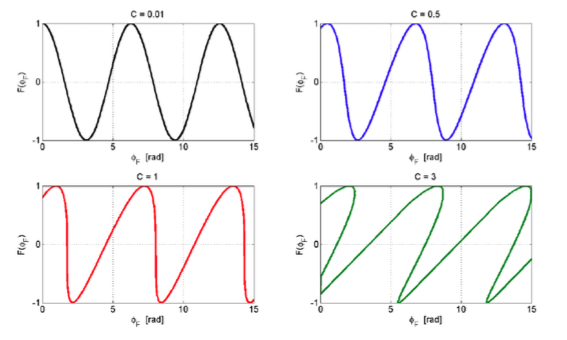
\includegraphics[scale=0.5]{cap2/regimifunz}
    \caption{Regimi di retroiniezione: funzione $F(\Phi)$ al variare del parametro $C$}
    \label{regimifunz}
  \end{center}
\end{figure}
\begin{figure}  
  \begin{center}
    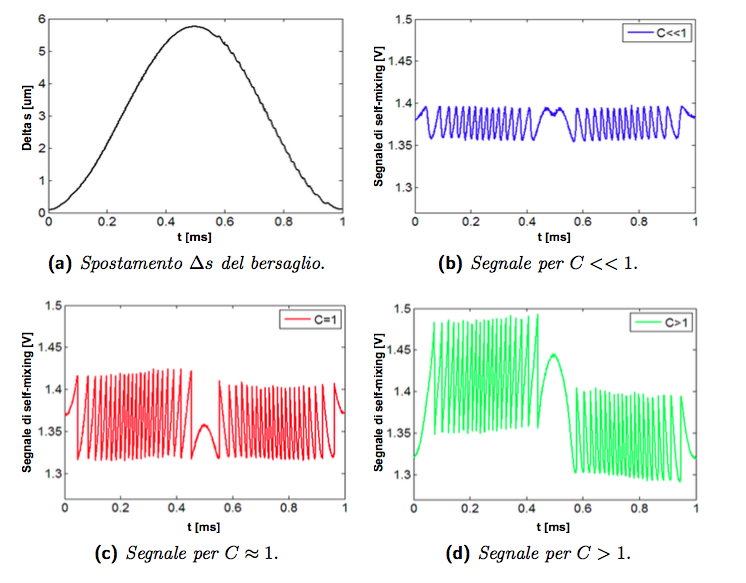
\includegraphics[scale=0.4]{cap2/regimisegn}
    \caption{Esempi di segnale interferometrico per i differenti valori del parametro $C$}
    \label{regimisegn}
  \end{center}
\end{figure}
In Figura \ref{regimifunz} è mostrata la forma della funzione $F(\Phi)$ nei 4 possibili regimi di funzionamento. Nella Figura \ref{regimisegn} è mostrato, invece, il segnale di comando del bersaglio e i rispettivi segnali interferometrici a frange al variare del parametro $C$.

Il segnale risultante è periodico in $\Phi$ e mostra le tipiche frange interferometriche ogni volta che la fase varia di $2\pi$. Ciascuna frangia corrisponde ad uno spostamento $\frac{\lambda}{2}$ del bersaglio~\cite{341714}.

\subsection{Vantaggi e svantaggi dell'interferometria a retroiniezione}
La tecnica self-mixing ha diversi vantaggi rispetto agli strumenti basati su altri principi, come i telemetri visti nel Capitolo precedente.

I principali vantaggi sono:
\begin{itemize}
	\item \underline{Semplicità strutturale}: Il sistema interferometrico non necessita dell'uso di un canale ottico di riferimento o di divisori di fascio. L'informazione dello spostamento è ricavata direttamente dalla potenza emessa dal laser.
	\item \underline{Semplicità di rilevamento}: Il rilevamento si basa sull'osservazione della distorsione delle frange, più semplice del rilevamento nell'interferometro di \textit{Michelson}. Inoltre, l'allineamento ottico del bersaglio non è particolarmente critico ed è possibile eseguire misure valide su molteplici tipologie di superficie del bersaglio.
	\item \underline{Performante}: La semplicità di rilevamento permette di ottenere uno strumento di misura performante.
	\item \underline{Non ambiguità del verso dello spostamento}: Il problema dell'ambiguità del verso di spostamento non è presente perché tale informazione è intrinseca nella forma d'onda $F(\Phi)$. Per tale motivo non si rende necessario l'utilizzo di un secondo canale di misura interferometrico. 
	\item \underline{Elevata sensibilità}: Si basa su un sistema ottico coerente che estrae le informazioni dalla sorgente di luce, a differenza della tecnica di triangolazione.
\end{itemize}
Tuttavia, l'interferometria a retroiniezione presenta anche diversi svantaggi:
\begin{itemize}
	\item \underline{Salti di modo}: Sono dovuti a variazioni di corrente o di temperatura nei laser a semiconduttore. Essi influenzano negativamente la misura dell'interferometro, degradandone le prestazioni.
	\item \underline{Dipendenza della misura da variabili esterne}: Variabili esterne come temperatura e pompaggio di corrente incidono sulla lunghezza d'onda d'emissione del laser, grandezza dalla quale dipende direttamente la misura, causando una ridotta accuratezza della misura.
	\item \underline{Decadimento della luce coerente}: \'E possibile che la potenza retroiniettata passi a regimi di alta iniezione compromettendo le misure o, in casi limite, danneggiando irreparabilmente il laser. 
\end{itemize}

\section{Principali limitazioni della tecnica interferometrica}
Indipendentemente dalla configurazione di interferometro scelta, le prestazioni della tecnica intereferometrica presentano limiti dovuti a molteplici cause. Le principali sono descritte di seguito.
\begin{figure}  
  \begin{center}
    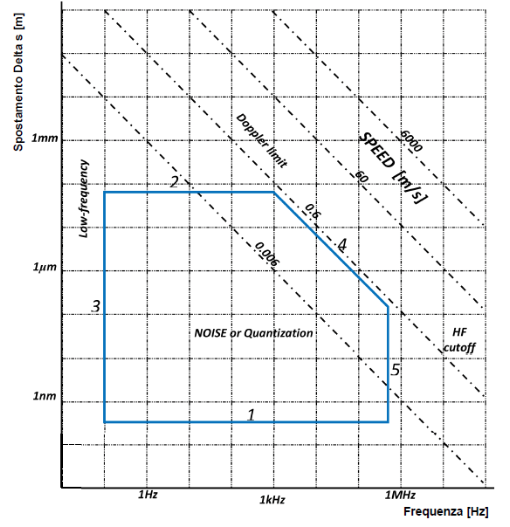
\includegraphics[scale=0.4]{cap2/wegel}
    \caption{Diagramma di Wegel}
    \label{wegel}
  \end{center}
\end{figure}
\begin{figure}  
  \begin{center}
    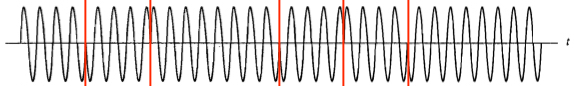
\includegraphics[scale=0.4]{cap2/saltifase}
    \caption{Esempio di salti di fase dell'onda nel tempo}
    \label{saltifase}
  \end{center}
\end{figure}
\begin{figure}  
  \begin{center}
    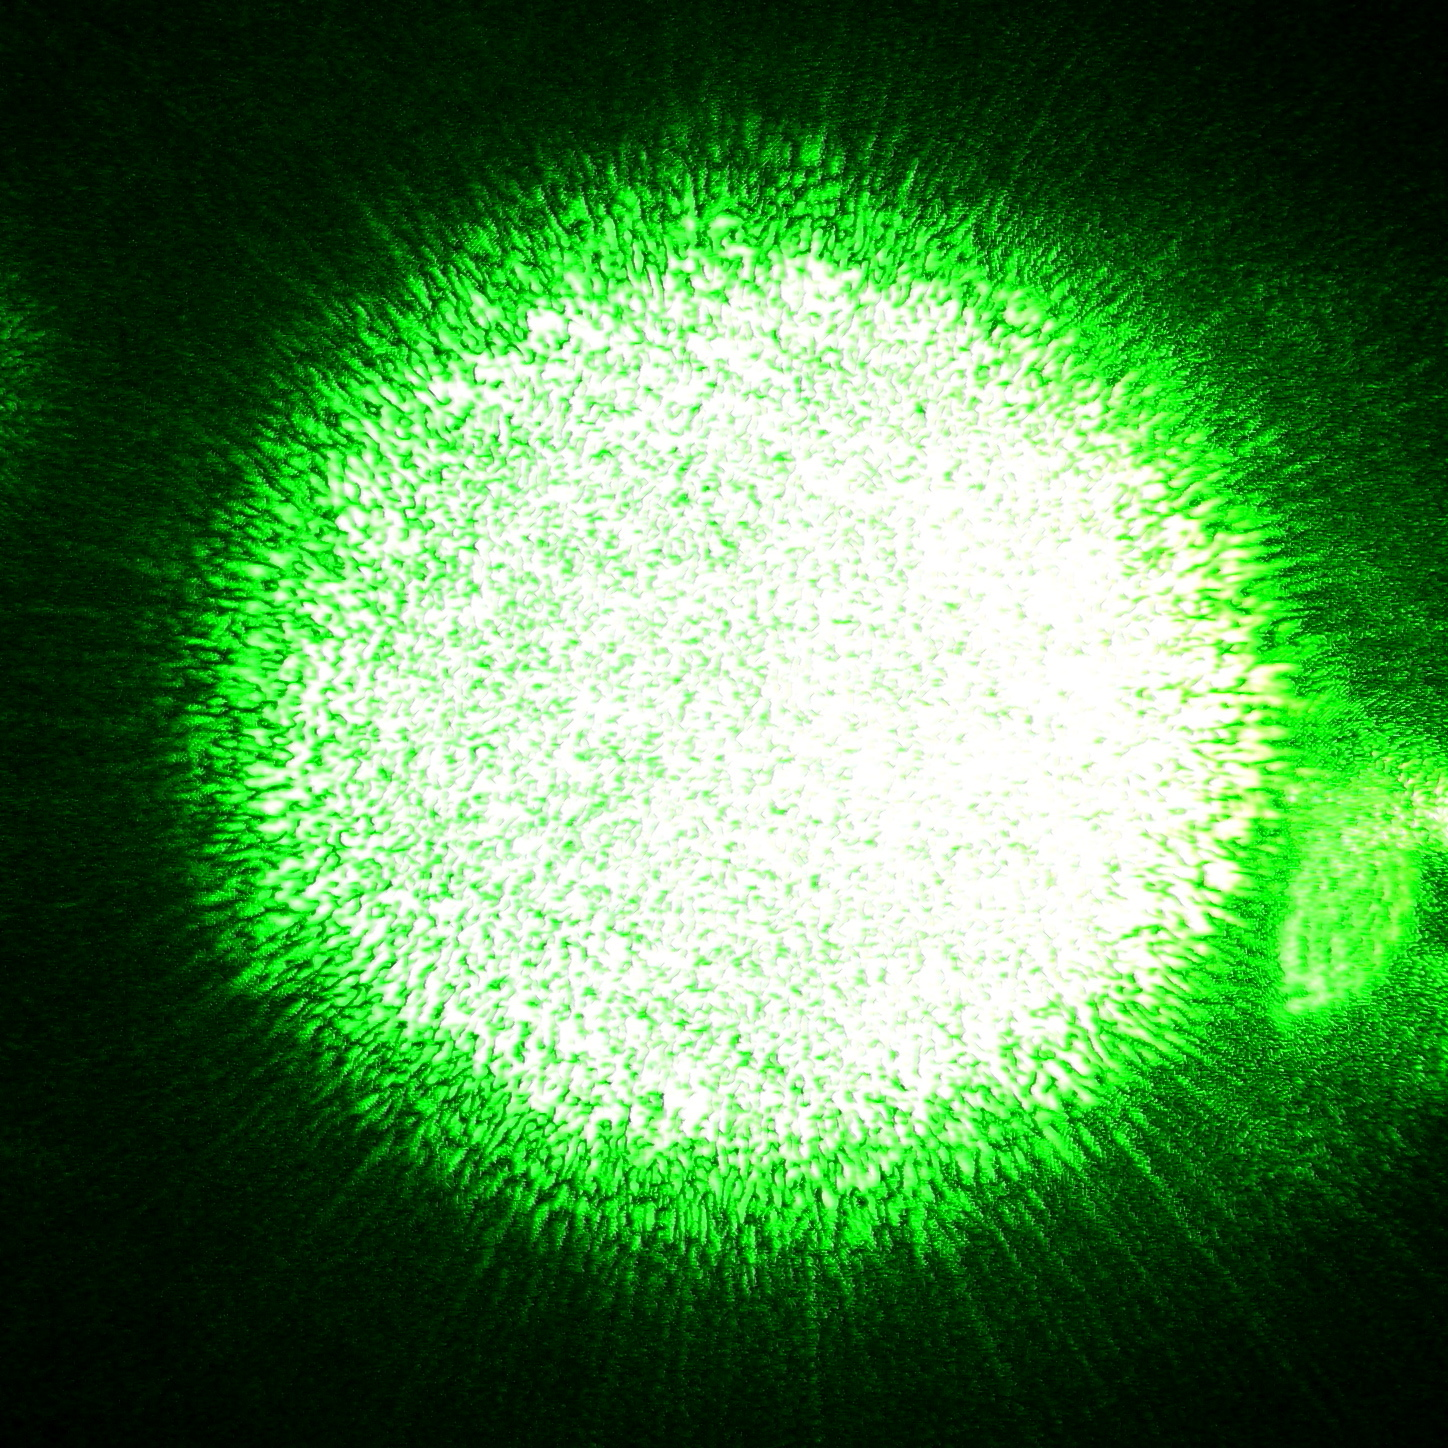
\includegraphics[scale=0.1]{cap2/spackle}
    \caption{Speckle causato da una superficie diffusiva}
    \label{spackle}
  \end{center}
\end{figure}
\begin{itemize}
	\item \underline{Limitazioni nel piano spostamento-frequenza}: Il diagramma di Wegel, rappresentato in Figura \ref{wegel}, è utilizzato per analizzare la qualità di un interferometro in termini di prestazioni e limiti. Il diagramma presenta 5 segmenti che delimitano un'area chiamata "zona di funzionamento". Maggiore sarà l'area della zona di funzionamento maggiore risulterà il campo d'azione dello strumento di misura.
 
		I 5 segmenti rappresentano, in particolare, 5 limitazioni qui di seguito riportate:
		\begin{itemize}
		\item \textit{Minimo spostamento misurabile}: Il segmento inferiore 1 definisce la sensibilità dello strumento al minimo spostamento misurabile in base al rumore elettronico di fondo.
		\item \textit{Massimo spostamento misurabile}: Il segmento superiore 2 impone il limite massimo di spostamento del bersaglio affinché lo strumento funzioni correttamente.
		\item \textit{Frequenza minima dello spostamento}: Il segmento laterale sinistro 3 indica la minima frequenza di vibrazione in accordo con la minima banda di segnale dell'elettronica di elaborazione.
		\item \textit{Frequenza massima dello spostamento}: Il segmento laterale destro 5 indica la massima frequenza di vibrazione in accordo con la massima banda di segnale dell'elettronica di elaborazione.
		\item \textit{Velocità di spostamento massima}: Il segmento obliquo 4 mostra la velocità limite di spostamento massimo, che è proporzionale al prodotto tra la frequenza di oscillazione e la sua ampiezza.
		\end{itemize}
	
	\item \underline{Coerenza temporale}: Un qualunque fascio coerente generato da un laser ha una lunghezza di coerenza limitata, ovvero dopo un certo tempo dalla sua emissione la fase dell'onda cambia ed assume un valore casuale. Dunque il campo emesso da un laser presenta salti di fase a intervalli casuali, come mostrato in Figura \ref{saltifase}. Indicando con $T_{coh}$ la coerenza temporale e con $L_{coh}$ la lunghezza di coerenza, è possibile scrivere:
		\begin{equation}
			\begin{cases}
				L_{coh}=cT_{coh}\\T_{coh}=\frac{1}{\Delta \nu}
			\end{cases}
		\end{equation}
		dove $c$ è la velocità della luce nel vuoto e $\Delta \nu$ è la larghezza di riga in frequenza.
		
		Dalle precedenti relazioni è possibile ricavare la distanza massima dell'ostacolo affinché non si perda la proprietà di coerenza:
		\begin{equation}
			s_{max}=|s_m - s_r|_{max}=\frac{c}{\Delta \nu} = L_{coh}
		\end{equation}
		Se la distanza dell'ostacolo è maggiore di $L_{coh}$ non si ha segnale interferometrico ma solo rumore dunque non è possibile effettuare misure valide non potendo contare correttamente le frange interferometriche. Questo rumore è definito come rumore di fase. Solitamente il rumore di fase è il contributo dominante nella determinazione del minimo spostamento misurabile. 
		
		Tuttavia esiste un altro contributo che limita le prestazioni: il rumore quantico. Tale rumore risulta essere quasi sempre trascurabile perché il rumore di fase è dominante rispetto ad esso.
		\item \underline{Speckle-Pattern}: \'E un fenomeno dovuto alla superficie del bersaglio. In particolare, se un fascio di luce coerente colpisce un bersaglio avente superficie diffondente la luce retrodiffusa avrà una distribuzione di potenza granulare e non omogenea. Il fenomeno è mostrato in Figura \ref{spackle}.
		
			La luce retrodiffusa è generata dalla combinazione di due fasci di luce: una porzione di fascio riflessa in modo speculare alla direzione di incidenza e l'altra porzione di fascio diffusa uniformemente nello spazio. Quest'ultima è causata da imperfezioni superficiali del bersaglio.
			
			Ogni imperfezione superficiale, chiamata avvallamento, si comporta come un diffusore di luce secondario debolmente correlato ad un avvallamento adiacente. Il campo risultante, in un punto $P$ difronte alla superficie dell'ostacolo, è formato dalla sovrapposizione delle onde generate da ciascun avvallamento.
			
			 L'effetto di tale sovrapposizione è il risultato dell'interferenza costruttiva e distruttiva di onde aventi fase diversa. Ogni granulo ottico così formato prende il nome di \textit{speckle}. Geometricamente si definisce \textit{speckle} un ellissoide avente variazioni di fase contenute nel $50\%$ e dimensioni trasversali ($S_t$) e longitudinali ($S_l$) pari a:
			 \begin{equation}
			 	S_t=\lambda \left ( \frac{z_0}{D} \right )^2
			 \end{equation}
			 \begin{equation}
			 	S_l=\lambda \left ( 2 \frac{z_0}{D} \right )^2
			 \end{equation}
			 dove $z_0$ è la distanza tra il punto di osservazione e il bersaglio e $D$ è la dimensione di macchia su di esso.
			 
			 Nelle misure basate sulla tecnica di interferometria a retroiniezione, lo \textit{speckle-pattern} rappresenta il fattore limitante più grande. A causa di tale disturbo, il segnale interferometrico risulterà interrotto ogni qual volta che il fascio di luce incontrerà uno \textit{speckle}. \'E possibile limitare questa problematica aumentando la potenza ottica retro-iniettata o adottando il sistema ottico più adatto per l'applicazione in questione.
	\item \underline{Dispersione del mezzo}: Il fascio ottico che si propaga fuori cavità subisce delle alterazioni dovute alle caratteristiche di ogni mezzo che esso attraversa, che ne modifica la lunghezza d'onda. I fattori che incidono maggiormente sono temperatura e pressione del mezzo. Per minimizzare il contributo dispersivo di questi fattori vengono impiegati stabilizzatori di temperatura e pressione ambientale.
\end{itemize}

\begin{figure}  
  \begin{center}
    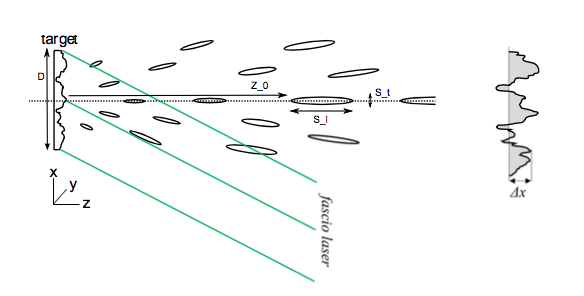
\includegraphics[scale=0.5]{cap2/specklegeom}
    \caption{Rappresentazione esemplificata del fenomeno dello speckle-pattern}
    \label{specklegeom}
  \end{center}
\end{figure}

\section{Applicazioni dell'interferometria a retroiniezione}
La tecnica interferometrica a retroiniezione può essere utilizzata in quattro principali campi di applicazione:
\begin{itemize}
	\item \underline{Misura di distanza assoluta}: Tecnica per la misurazione di distanza tra lo strumento di misura e un oggetto remoto (bersaglio).
	\item \underline{Velocimetria}: Tecnica per la misurazione di velocità a distanza.
	\item \underline{Vibrometria}: Tecnica per la misurazione delle vibrazioni. Il vibrometro laser è utile quando non è possibile installare un accelerometro sull'oggetto da misurare. Si basa sul principio di aggancio di fase~\cite{thesismelch}.
	\item \underline{Misura di spostamenti}: Tecnica per la misurazione dello spostamento di un bersaglio. Si basa sul conteggio delle frange interferometriche di periodicità $\frac{\lambda}{2}$ al variare della distanza dal bersaglio.
\end{itemize}

La misura di distanza assoluta, oggetto del seguente lavoro di Tesi, verrà discussa ampiamente nel paragrafo successivo.

\subsection{Misura di distanza assoluta}
Come descritto in precedenza, un segnale interferometrico è caratterizzato dalla seguente relazione:
\begin{equation}
	\phi = 2ks = 2 \frac{2\pi}{\lambda}s
	\label{distass}
\end{equation}
che rappresenta lo sfasamento del campo elettrico retroiniettato rispetto al campo elettrico emesso.

Da tale relazione si nota che per generare un segnale interferometrico è necessario uno spostamento $s$ del bersaglio o una variazione della lunghezza d'onda $\lambda$ del fascio emesso dal laser. Considerando come campo di applicazione la misura di distanza assoluta è necessario agire solo sulla lunghezza d'onda $\lambda$ e non sullo spostamento $s$ dato che il bersaglio è immobile.

Un metodo per variare la lunghezza d'onda $\lambda$ è quello di modulare la corrente di pompa della sorgente laser:
\begin{equation}
		\lambda_{new}=\lambda_{old}+\chi\Delta I
		\label{lungondanew}
\end{equation}
dove $\chi$ è la variazione di lunghezza d'onda rispetto alla variazione di corrente. La variazione di lunghezza d'onda $\chi$ è pari a $\chi = \frac{\Delta \lambda}{\Delta I}$ ed è espressa in $\left [ \frac{pm}{mA} \right ]$. Tale parametro varia molto da dispositivo a dispositivo. Esso risulta, inoltre, fortemente non lineare in alcune zone di funzionamento della sorgente laser. 

Differenziando l'equazione \ref{lungondanew}, rispetto alla lunghezza d'onda $\lambda$, è possibile ottenere la variazione di fase del segnale interferometrico:
\begin{equation}
	\frac{d\phi}{d\lambda}=-2\frac{2\pi}{\lambda^2}s
\end{equation}
da cui si può ricavare la misura di distanza assoluta $s$:
\begin{equation}
	s=-\frac{d\phi}{d\lambda}\frac{\lambda^2}{4\pi}
\end{equation}
Infine, la misura di distanza assoluta s può essere compiuta in due modi:
\begin{enumerate}
	\item \underline{Conteggio del numero di frange}: Questo metodo consiste nel contare il numero di frange visibili nel segnale interferometrico. Il numero di frange ad una distanza fissata $s$ dipende dalla variazione della lunghezza d'onda. Nota la variazione della lunghezza d'onda, più precisamente il periodo in cui viene fornita la variazione di corrente che genera la variazione di lunghezza d'onda, è possibile misurare la distanza assoluta del bersaglio con la seguente equazione:
	\begin{equation}
		s=\frac{N_F}{\Delta \lambda}\frac{\lambda^2}{2}
	\end{equation}
	dove $N_F$ rappresenta il numero di frange pari a:
	\begin{equation}
		N_F=\frac{\Delta \phi}{2 \pi}
	\end{equation}
	Questo metodo ha una scarsa accuratezza poiché la risoluzione massima ottenibile è data dalla singola frangia. 
	\item \underline{Misura del tempo di frangia}: Questo metodo consiste nella misura del periodo di frangia. Definendo con $t_{frangia}$ la lunghezza del periodo di frangia, è possibile scrivere la seguente proporzione:
	\begin{equation}
		\Delta \lambda_{2\pi} : \Delta \lambda = t_{frangia} : \Delta t
	\end{equation}
	dove $\Delta \lambda_{2\pi}$ è la variazione di lunghezza d'onda 
che produce una variazione di fase interferometrica $\Delta \phi$ pari a $2\pi$.
	
	Dalla precedente relazione è possibile ricavare la variazione di lunghezza d'onda $\Delta \lambda_{2\pi}$:
	\begin{equation}
		\Delta \lambda_{2\pi} = \frac{t_{frangia}}{\delta t} \Delta \lambda = \frac{\Delta \lambda}{\Delta I}\frac{\Delta I}{\Delta t} t_{frangia}
	\end{equation}
	Per ricavare la distanza assoluta $s$ è necessario fare riferimento alla relazione:
	\begin{equation}
		2\frac{2\pi}{\lambda}-2\frac{2\pi}{\lambda + \Delta \lambda_{2\pi}} s = 2\pi
	\end{equation}
	che eguaglia la differenza di fase causata da una variazione di lunghezza d'onda $\Delta \lambda_{2\pi}$ a $2\pi$.
	
	Infine, per ricavare la distanza $s$, è necessario approssimare $\lambda + \Delta \lambda_{2\pi} \approx \lambda$ poiché $\lambda \gg \Delta \lambda_{2\pi}$:
	\begin{equation}
		s \approx \frac{\lambda^2}{2\frac{\Delta \lambda}{\Delta I}\frac{\Delta I}{\Delta t} t_{frangia}} =  \frac{\lambda^2}{2\frac{\Delta \lambda}{\Delta I}\frac{\Delta I}{\Delta t}}f_{frangia}
	\end{equation}
	dove $f_{frangia}=\frac{1}{t_{frangia}}$ è il tono fondamentale del segnale interferometrico.
	
	Lo strumento di misura descritto in questo elaborato, deve essere in grado di effettuare la misura anche con ostacolo in movimento. Per tale motivo occorre scegliere un'opportuna forma d'onda per realizzare la modulazione in corrente.
	
	Come già detto in precedenza, uno spostamento dell'ostacolo provoca una variazione di fase del segnale interferometrico. Richiamando che la variazione di fase causata dalla modulazione equivale a:
	\begin{equation}
		\frac{d\phi_{mod}}{dt} = 2 \pi f_{mod}
	\end{equation}
	e derivando la relazione \ref{distass} rispetto allo spazio:
	\begin{equation}
		\frac{d\phi_s}{ds}=2\frac{2\pi}{\lambda}
	\end{equation}
	è possibile ottenere:
	\begin{equation}
		\frac{d\phi_s}{ds}=2\pi f_s
	\end{equation}
	dove $f_s$' è la frequenza media delle frange prodotte a causa dello spostamento.
	
	Da questo si deduce che: se il bersaglio è in movimento la variazione di fase complessiva del segnale interferometrico è data dalla somma di due componenti: $\phi_{mod}$ e $\phi_s$.
	Per compensare il contributo indesiderato $\phi_s$ è necessario realizzare una modulazione di corrente che vada a incrementare e decrementare la lunghezza d'onda della sorgente laser. Per fare ciò, si utilizza un segnale a forma triangolare con ampiezza opportuna.
	
	Un accorgimento atto a compensare e minimizzare gli sfasamenti consiste nell'esecuzione, durante il processo di misura, di una media tra il periodo di frangia valutato nella fase ascendente e il periodo di frangia valutato nella fase discendente della triangolare di modulazione allo scopo di aumentare la sensibilità dello strumento rispetto allo spostamento. 
	
Da questa osservazione si ottiene la relazione:
\begin{equation}
	s \propto \frac{f_{rise}+f_{fall}}{2} = \frac{ \left | \frac{d\phi_{rise}}{dt} + \frac{d\phi_{fall}}{dt} \right |}{2}
	\label{eqrisefall}
\end{equation}
dove $f_{rise}$ e $f_{fall}$ sono rispettivamente il tono fondamentale del segnale interferometrico nella rampa di salita e discesa dell'onda triangolare.

Sapendo che la fase complessiva del segnale interferometrico è formata dai due contributi discussi in precedenza è possibile sostituire nella relazione \ref{eqrisefall} la fase totale $\phi_{tot} = \phi_{mod} + \phi_s$:
\begin{equation}
	s \propto \frac{ \left | \frac{d\phi_{mod}}{dt} + \frac{d\phi_{s}}{dt} \right |+ \left | \frac{d\phi_{mod}}{dt} - \frac{d\phi_{s}}{dt} \right |}{2} = \frac{d\phi_{mod}}{dt}
\end{equation}
Infine, in questo modo è possibile misurare la distanza assoluta eliminando così il contributo indesiderato $\phi_s$ causato da un eventuale spostamento del bersaglio.

Esprimendo le grandezze $f_{rise}$ e $f_{fall}$ attraverso le seguenti relazioni:
\begin{equation}
	f_{rise}= \left | \frac{1}{2\pi} \frac{\delta \phi}{\delta t} \right | = \left | - \frac{2s}{\lambda^2} \frac{\delta \lambda}{\delta t} + \frac{2}{\lambda} \frac{\delta s}{\delta t} \right | = \left | - \frac{2sk}{\lambda^2} \frac{\Delta I}{\Delta T} + \frac{2}{\lambda}v \right |
\end{equation}
\begin{equation}
	f_{fall}= \left | \frac{1}{2\pi} \frac{\delta \phi}{\delta t} \right | = \left | \frac{2s}{\lambda^2} \frac{\delta \lambda}{\delta t} + \frac{2}{\lambda} \frac{\delta s}{\delta t} \right | = \left | \frac{2sk}{\lambda^2} \frac{\Delta I}{\Delta T} + \frac{2}{\lambda}v \right |
\end{equation}
dove $v$ è la velocità del bersaglio e $T$ è il semiperiodo della triangolare di modulazione, è possibile definire l'equazione della distanza assoluta $s$ in maniera più precisa:
\begin{equation}
	s = \frac{f_{rise}+f_{fall}}{2} \left [ \frac{\lambda^2}{2k\left ( \frac{\Delta I}{\Delta T} \right )}  \right ]
\end{equation}
Questa tecnica risulta più accurata della precedente perché è limitata solamente dalla precisione con la quale è possibile misurare il periodo e dalla capacità della sorgente di generare un segnale interferometrico ripetibile. 

\end{enumerate}

%%TODO Cap 2: Controllare le formule
\chapter{Architettura Hardware dello strumento}
\label{capitolo3}
\thispagestyle{empty}

\noindent %%TODO Cap 3


\chapter{Architettura Software dello strumento}
\label{capitolo4}
\thispagestyle{empty}

\textit{In questo Capitolo verrà descritta l’architettura software dello strumento realizzato. Inizialmente verrà analizzato l’ambiente di sviluppo software. Successivamente verrano mostrati i principi alla base della programmazione per microcontrollore e FPGA. Infine, verranno illustrate e descritte le funzionalità implementate su microcontrollore ed FPGA.}

\section{Ambiente di sviluppo LabVIEW}
%%TODO Cap 4
\section{Sistema Real-Time e FPGA}

	\subsection{Sistema Real-Time}

		\subsubsection{Sistema Operativo Real-Time}

			\paragraph{VxWorks}

		\subsubsection{LabVIEW Real-Time}

	\subsection{Progettazione e programmazione dell'FPGA}
		
		\subsubsection{Linguaggi di descrizione dell'Hardware (HDL)}
		
		\subsubsection{Sintesi Hardware}
		
		\subsubsection{High-Level Synthesis (HLS)}
		
		\subsubsection{LabVIEW FPGA}
		
\section{Analisi teorica degli algoritmi implementati}

	\subsection{Algoritmo di FFT}
		
	\subsection{Algoritmo di FFT Interpolata}
		
	\subsection{Misura di distanza}
	
\section{Architettura Software}

	\subsection{FPGA}
	
		\subsubsection{Implementazione software}
		
			\paragraph{Design pattern utilizzati}
		
				\subparagraph{Producer-consumer}
			
				\subparagraph{4-Wire Handshake}
			
			\paragraph{Fixed Point}
	
	\subsection{Microcontrollore}
	
		\subsubsection{Implementazione software}
	
	\subsection{Comunicazione tra FPGA e Microcontrollore}
		
		




\chapter{Misure effettuate e dati sperimentali}
\label{capitolo5}
\thispagestyle{empty}

\textit{In questo Capitolo verranno presentati e commentati i risultati delle prove sperimentali svolte.}

\section{Metodologia proposta}
Per testare lo strumento e valutarne le prestazioni sono state effettuate tre differenti tipologie di prove.

La prima consiste nell'acquisire un certo numero di misure di un bersaglio fisso a distanza nota. La seconda tipologia, al contrario, si articola in due fasi. Inizialmente si acquisisce un campione della distanza del sensore da un bersaglio montato su una slitta motorizzata in grado di compiere spostamenti precisi; in seguito si procede spostando la slitta di una distanza nota, ripetendo il procedimento un numero prefissato di volte. Le due prove mirano a valutare differenti caratteristiche dello strumento: la precisione e l'accuratezza della misura.

Queste prove sono state effettuate inizialmente ad una distanza prefissata di $50cm$ e ripetute ad ogni passo dello sviluppo dello strumento. A strumento ultimato sono state effettuate due ulteriori misurazioni (a $20cm$ e a $90cm$), per valutare le prestazioni del prototipo finale su un range più vario di distanza.

La terza tipologia di prova, invece, si svolge mantenendo il bersaglio fisso ad una distanza prestabilita e acquisendo un numero di campioni coerente con quello che lo strumento finale userà per fornire all'utente un singolo campione di distanza. In seguito si varia la distanza del bersaglio dal sensore e si ripete l'acquisizione. Lo scopo della prova è valutare empiricamente il range di misura dello strumento.

Per tutte le prove il fuoco del laser è stato mantenuto oltre la massima distanza misurata in ciascuna prova.

Di seguito sono descritte più nel dettaglio le metodologie di prove effettuate. Per confrontare i miglioramenti tra diverse implementazioni si è scelto di valutare la deviazione standard  (o incertezza) relativa della misura.

\begin{figure}
  \begin{center}
  	%% TODO Cap5 Riusciamo a sistemare sta foto?
    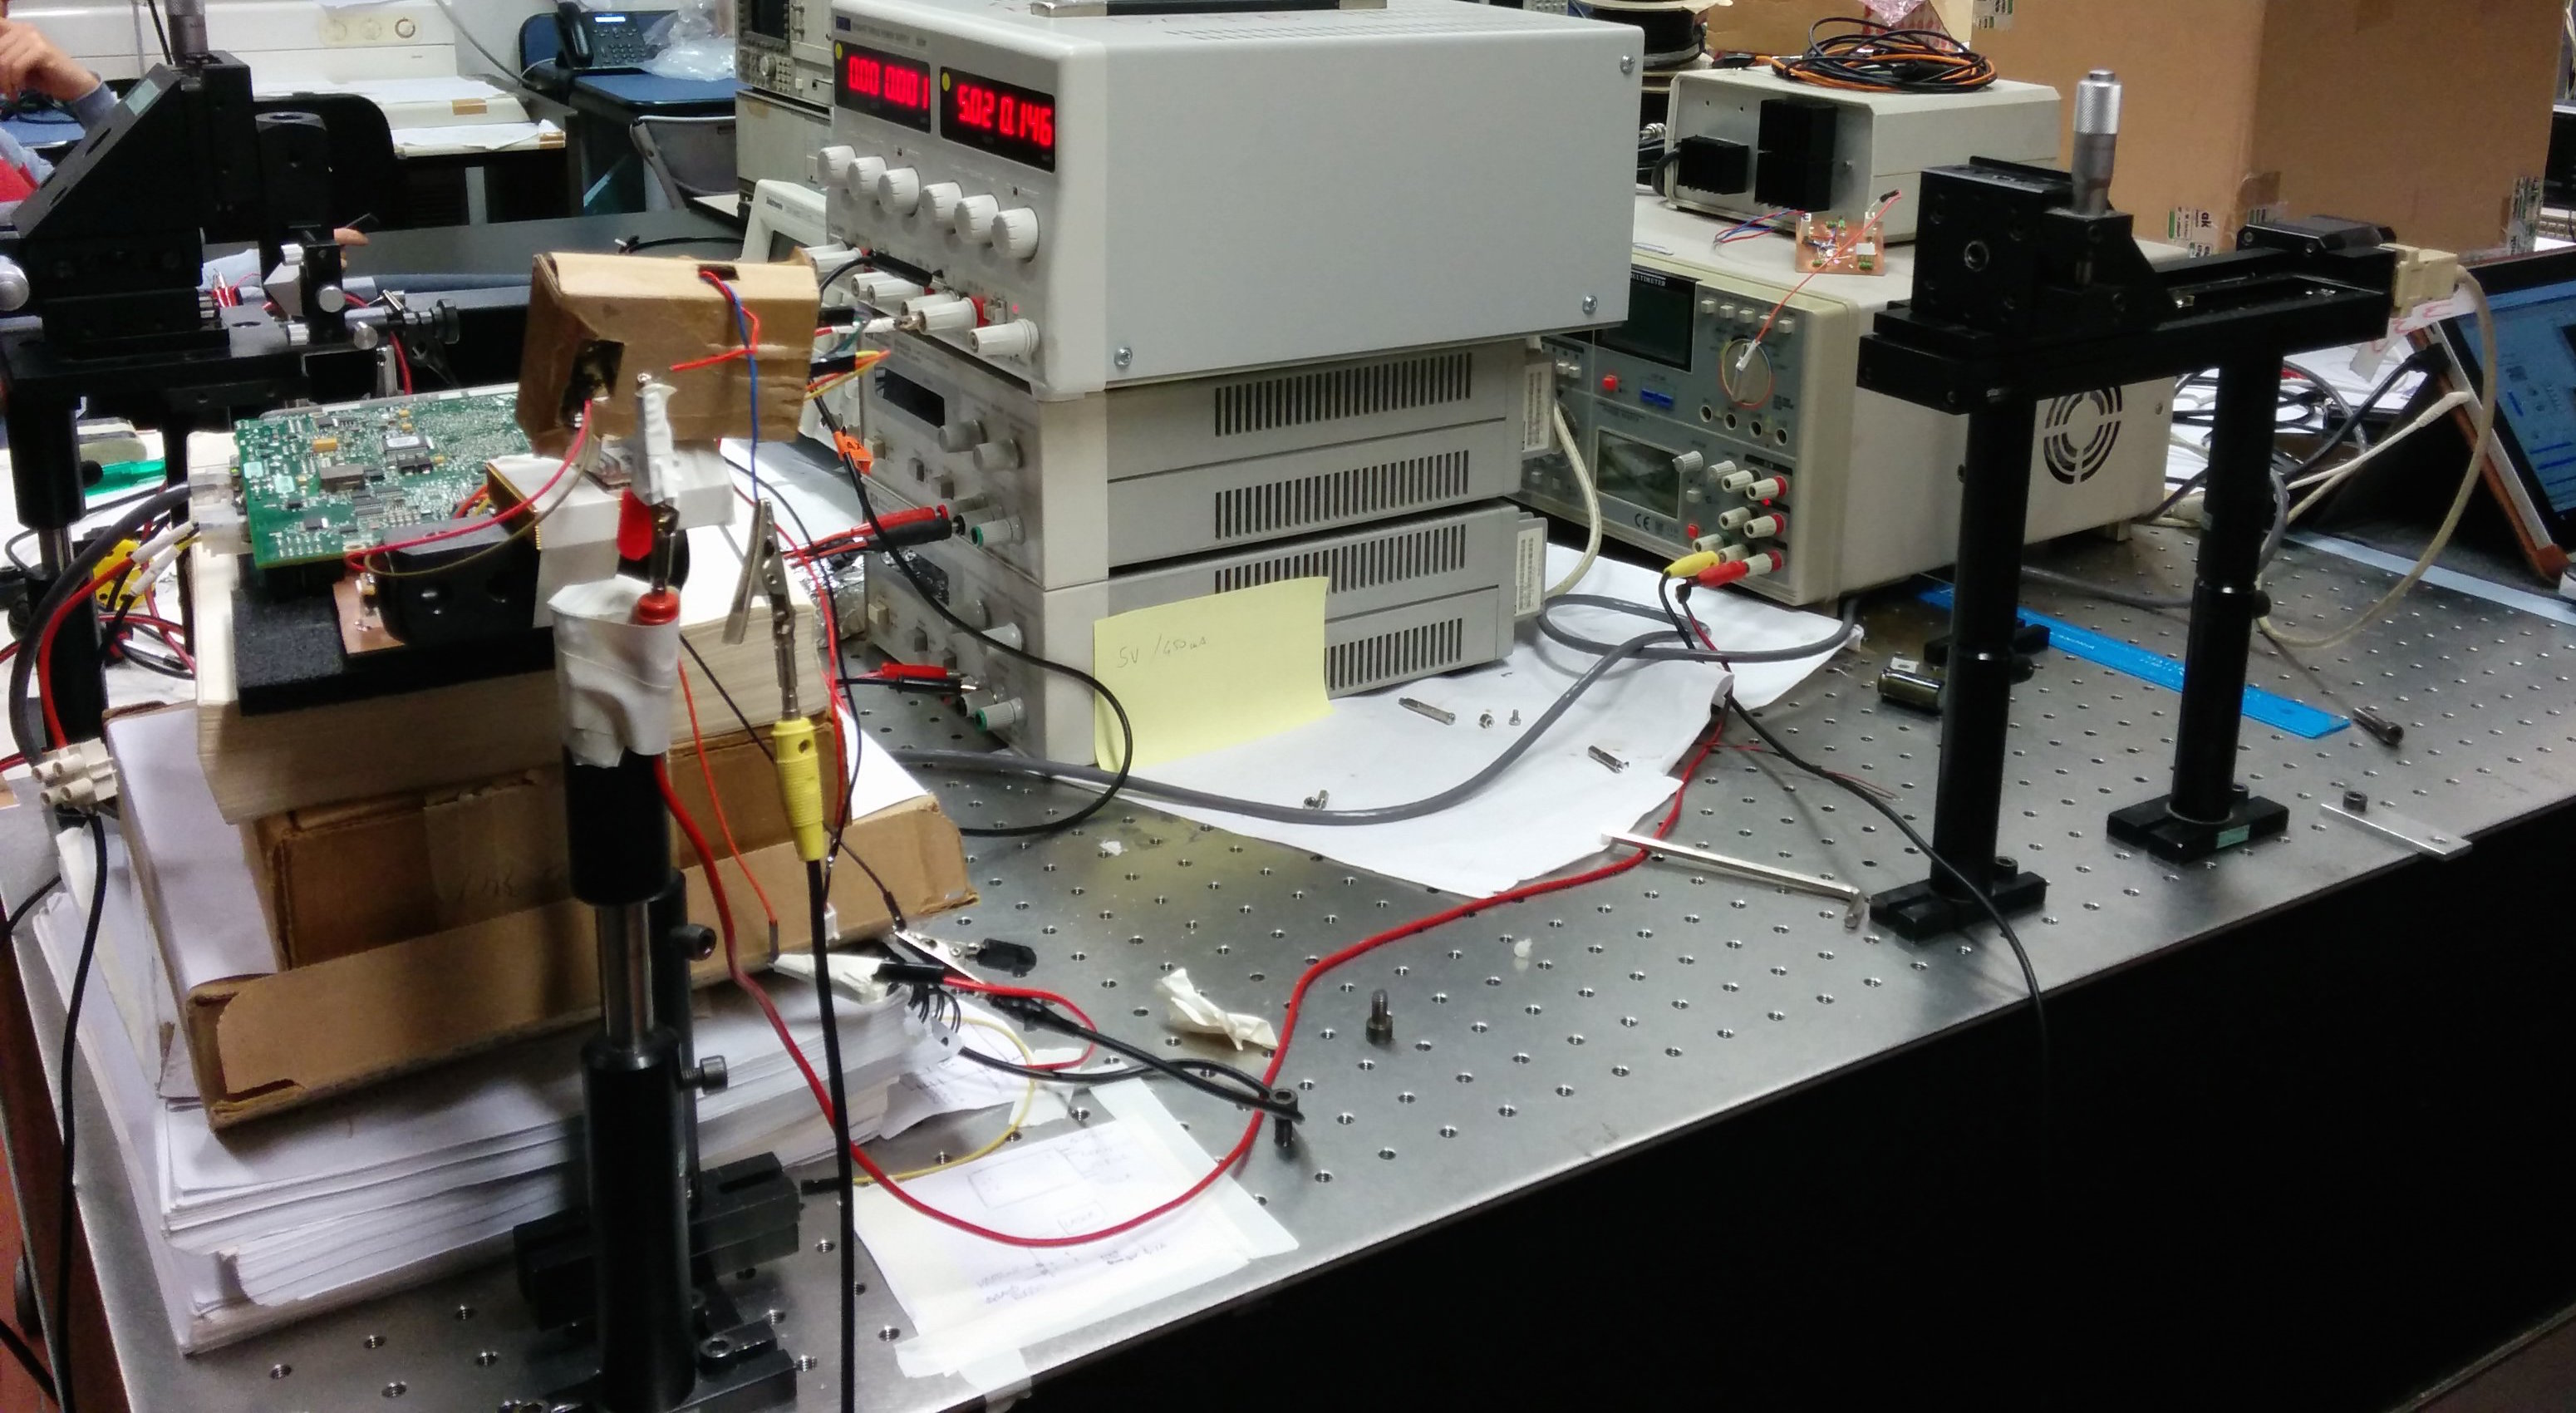
\includegraphics[scale=0.1]{cap5/allestimento}
    \caption{Allestimento della misura}
  \end{center}
\end{figure}

\subsection{Prova a bersaglio fisso}
La misura a bersaglio fisso è stata effettuata con il sensore fissato su di un tavolo ottico e puntato verso un bersaglio metallico nero, anch'esso fissato ad un tavolo ottico. L'uso del tavolo ottico si è reso necessario per minimizzare l'effetto delle vibrazioni.

Inizialmente si è lasciato in esecuzione il software che effettua la modulazione del laser, in modo da consentire al sensore di raggiungere una temperatura stabile, per minimizzare l'influenza del cambiamento di temperatura del laser sulla misura. Si è deciso di lasciare attiva la modulazione senza acquisire dati per circa $10$ minuti.

Con lo strumento ad una temperatura stabile si sono acquisiti $1000$ campioni della distanza dal bersaglio e se ne è valutata la media e la deviazione standard relativa. In questo modo è stato possibile valutare quanto è ampia l'oscillazione della misura rispetto alla media, e di determinare così la precisione dello strumento.

La misura si ritiene più precisa tanto minore è la sua deviazione standard relativa.

\subsection{Prova a bersaglio mobile}
La misura a bersaglio mobile è stata effettuata con un allestimento simile alla prova precedente. L'unica differenza è stato il fissaggio del bersaglio ad una slitta micrometrica, codice prodotto \textit{STANDA 8MT175-150}, uno strumento in grado di eseguire spostamenti dell'ordine dei micrometri, con una precisione di $0.31 \mu m$ \cite{standa}.

La prova si articola in due fasi:
\begin{enumerate}
	\item Acquisizione
	\item Spostamento
\end{enumerate}
Nella fase di acquisizione, con il bersaglio fermo, si acquisiscono $100$ campioni della distanza dal sensore. Di questi campioni si valutano media e deviazione standard relativa.
Nella fase di spostamento si allontana la slitta di $200 \mu m$ dal sensore. Si è scelto di utilizzare un passo di $200 \mu m$ perché consistente con la risoluzione dello strumento verificata nella prova a bersaglio fisso.

Queste due fasi sono ripetute per $15 \div 20$ volte, in modo da coprire una distanza totale di $3 \div 4 mm$.

Lo scopo della prova è quello di valutare la linearità dello strumento rispetto allo spostamento del bersaglio. Per fare questo si valuta l'oscillazione della misura rispetto alla retta ideale dello spostamento; in particolare si valutano distanza picco-picco dell'errore della misura rispetto alla retta ideale e l'RMS (\textit{Root Mean Square}, valore quadratico medio).

L'errore di misura è calcolato in modo semplice con la relazione:
\begin{equation}
	e = x_t - x 
\end{equation}
Dove con $x_t$ si intende il punto teorico appartenente alla retta ideale del valor medio, e con $x$ si intende il punto misurato dal sensore. 

La distanza picco-picco dell'errore è misurata come:
\begin{equation}
	e_{pp} = max(e) - min(e)
\end{equation}

I risultati migliori si ottengono quando si riscontrano distanze picco-picco ed RMS minori.

\subsection{Prova del range di misura}
La prova del range di misura si effettua con un allestimento identico alla prima prova, ma, al contrario di quest'ultima, i campioni acquisiti sono in numero minore, ovvero $100$. Il numero è stato scelto in modo coerente con il numero di campioni che lo strumento finale utilizzerà per fornire all'utente un singolo valore di distanza. 

Poiché lo scopo della prova è valutare il range di distanze in cui lo strumento è in grado di lavorare nei limiti di precisione desiderati, si ripete l'acquisizione dei campioni a diverse distanze dal sensore, partendo da $10 cm$ e arrivando a $100 cm$, con passi di $10 cm$ circa.

Sui $100$ campioni acquisiti si valutano media e deviazione standard relativa, e si ritiene soddisfacente la prestazione dello strumento quando la deviazione standard relativa fornita è minore di $10^{-3}$.

\section{Finestratura del segnale}
Come già discusso nel Capitolo \ref{capitolo4}, l'implementazione finale dello strumento genera un'onda triangolare che modula la sorgente laser in corrente. 

L'onda di modulazione triangolare generata e il segnale interferometrico in risposta dal laser, sono formati entrambi da $1250$ punti, $625$ per il semiperiodo di discesa della triangolare di modulazione e $625$ per il semiperiodo di salita. 
\begin{figure}
  \begin{center}
    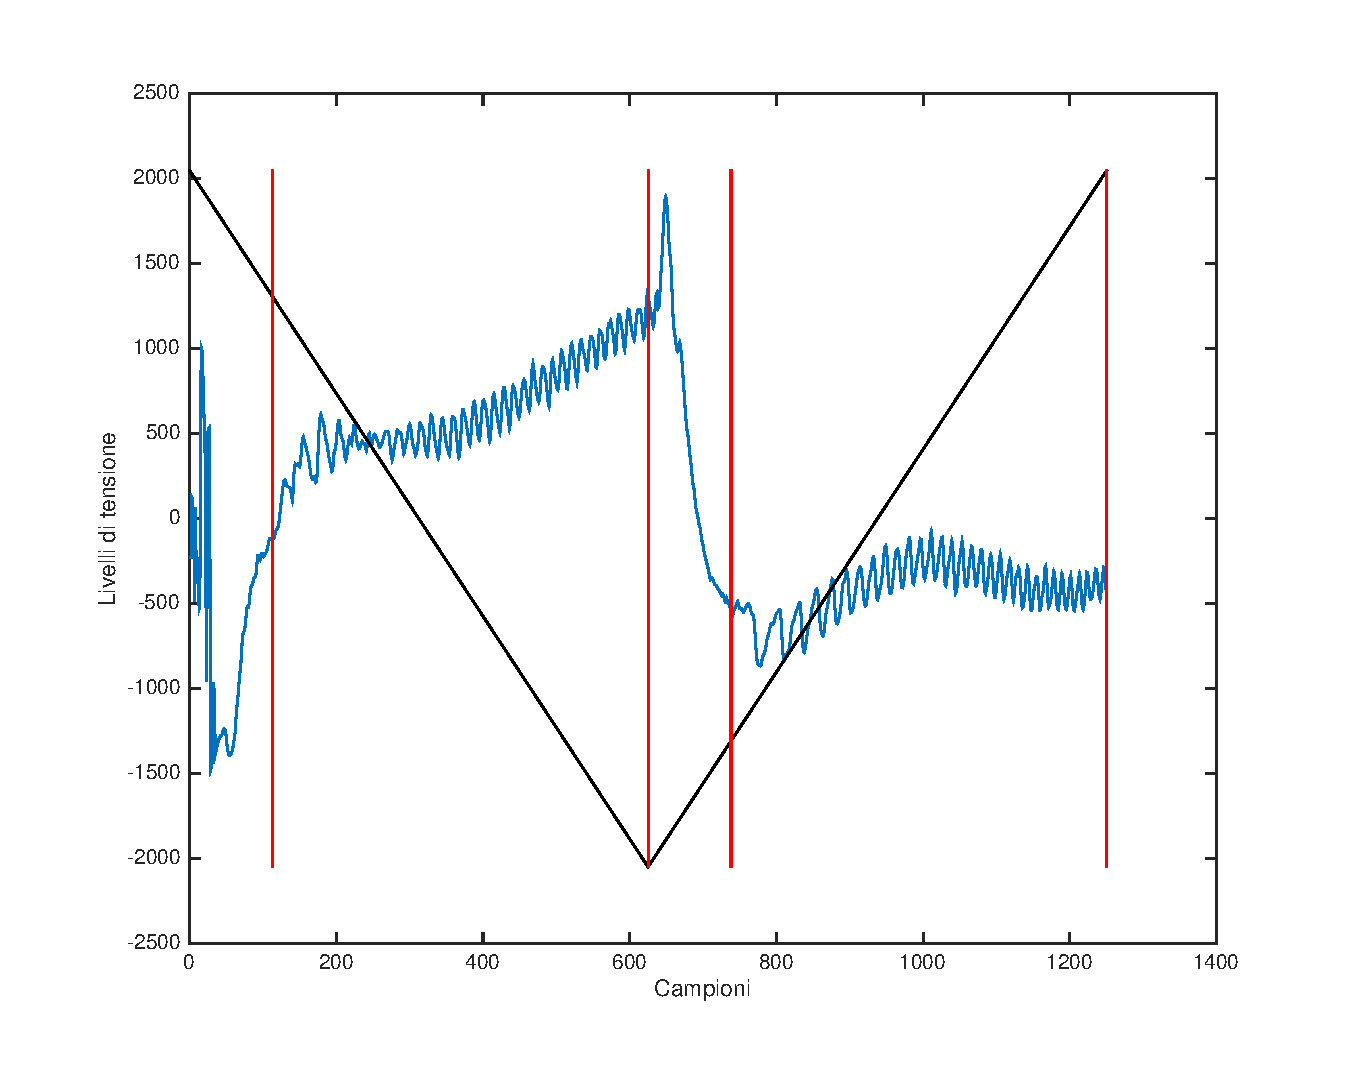
\includegraphics[scale=0.5]{cap5/segnaleinterf}
    \caption{Segnale interferometrico (blu) in un periodo di modulazione (nero)}
    \label{segnaleinterf}
  \end{center}
\end{figure}

Di questi $625$ punti soltanto $512$ contengono l'informazione utile per l'estrazione della frequenza interferometrica, poiché inizialmente si ha una parte di segnale influenzata dall'inversione del verso di polarizzazione del laser (Figura \ref{segnaleinterf}). 

Per l'estrazione del tono fondamentale del segnale si utilizza l'algoritmo di FFT interpolata a due punti con finestratura a $512$ punti.

Come accennato nel capitolo precedente, sono state valutate due differenti finestrature per il segnale: la finestra rettangolare e quella di \textit{Hanning}.

Per determinare quale delle due finestrature utilizzare nell'implementazione finale dello strumento sono state realizzate prove a bersaglio fisso e a bersaglio mobile con modulazione triangolare a pendenza fissa.
\begin{figure}
\centering
\subfigure[Misure di distanza e media]
{\label{misfisso1a}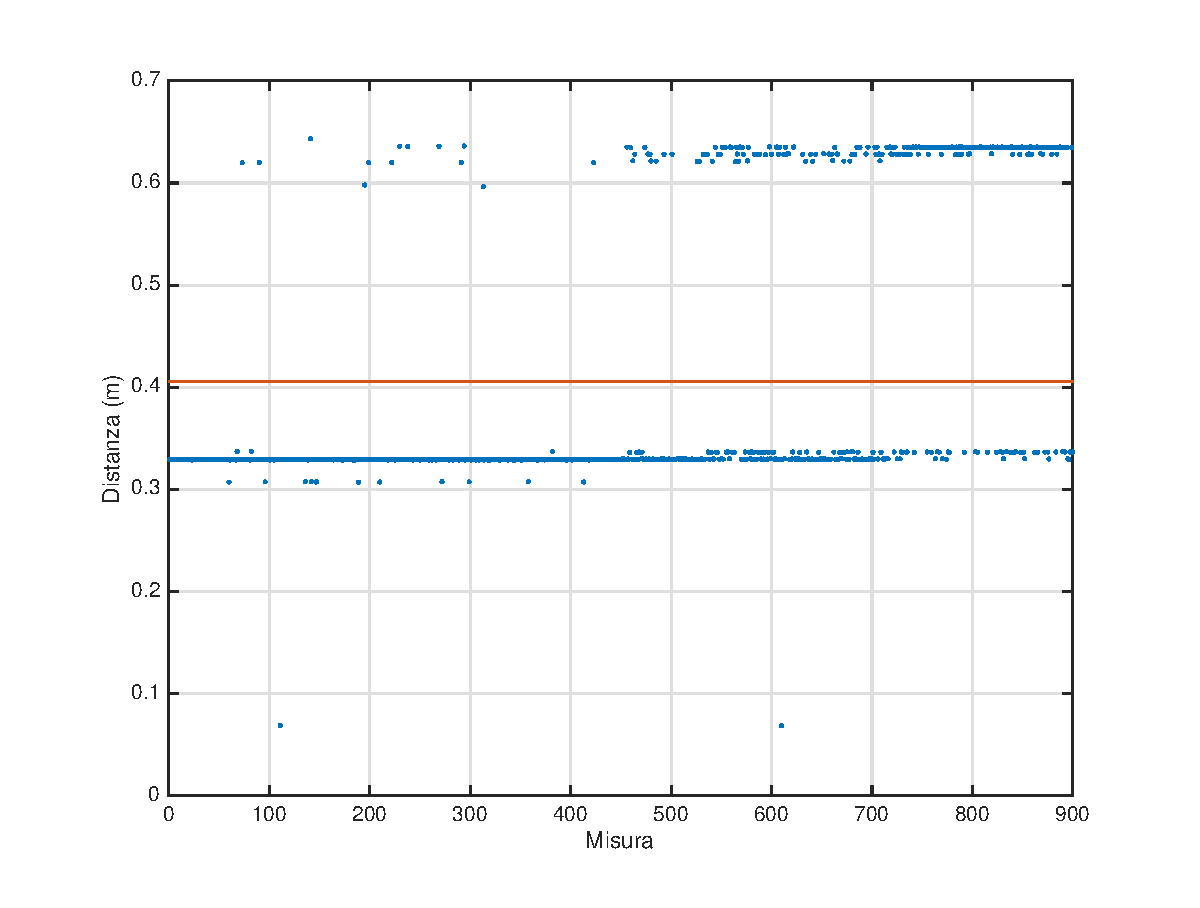
\includegraphics[scale=.5]{cap5/misfisso1a}}
\hspace{5mm}
\subfigure[Distribuzione dei valori misurati rispetto alla media]
{\label{misfisso1b}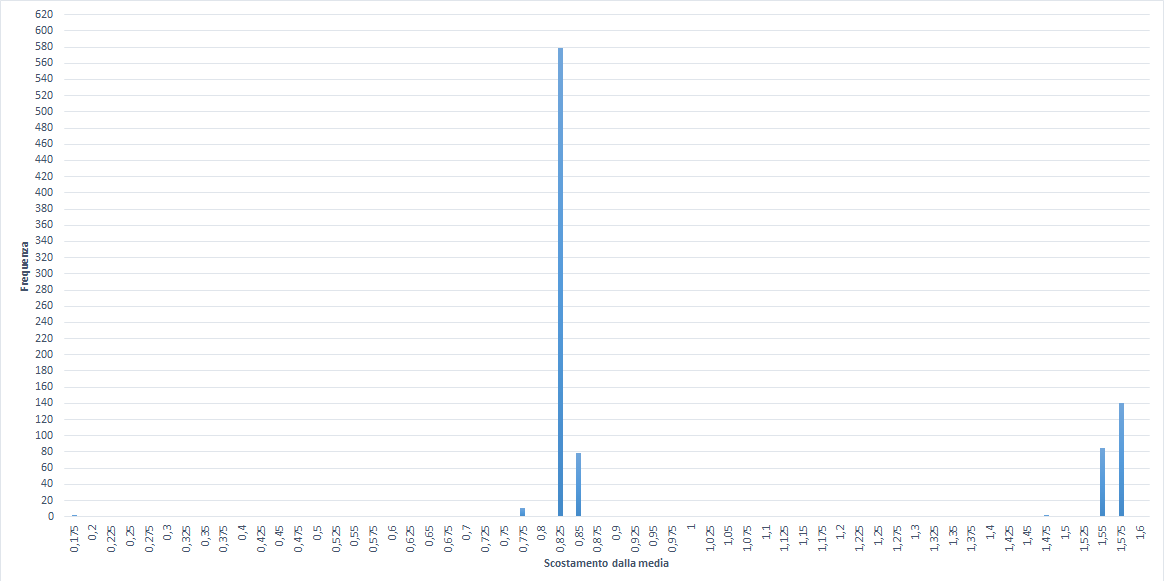
\includegraphics[scale=.4]{cap5/misfisso1b}}
\caption{Misure a bersaglio fisso con finestratura rettangolare}\label{misfisso1}
\end{figure}

\begin{figure}
\centering
\subfigure[Misure di distanza e media]
{\label{misfisso2a}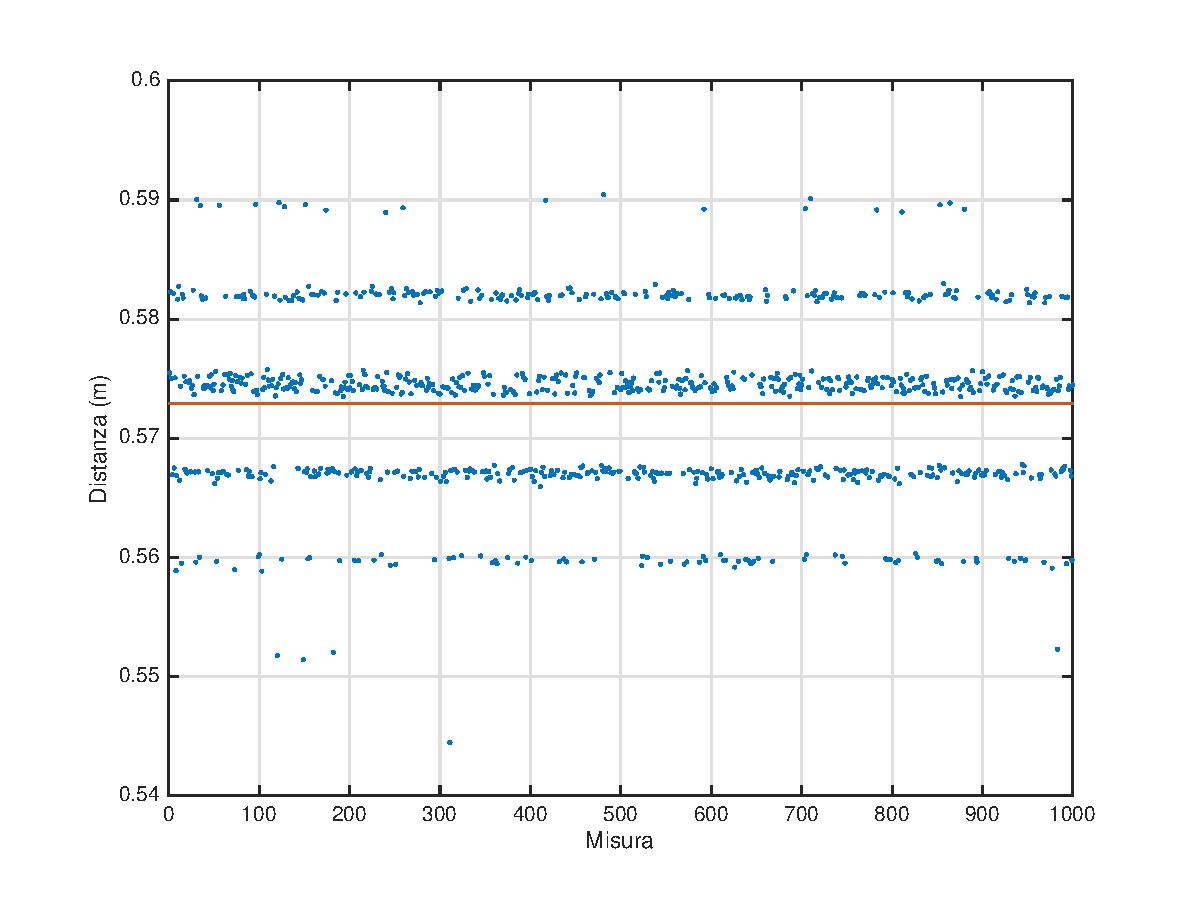
\includegraphics[scale=.5]{cap5/misfisso2a}}
\hspace{5mm}
\subfigure[Distribuzione dei valori misurati rispetto alla media]
{\label{misfisso2b}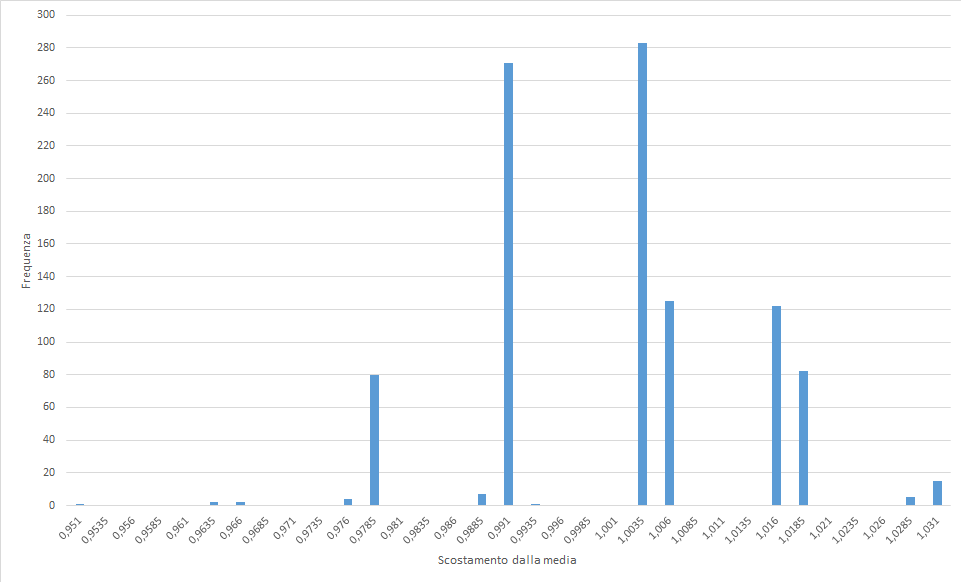
\includegraphics[scale=.5]{cap5/misfisso2b}}
\caption{Misure a bersaglio fisso con finestratura di Hanning}\label{misfisso2}
\end{figure}

\begin{figure}
\centering
\subfigure[con finestra rettangolare]
{\label{mismobile1}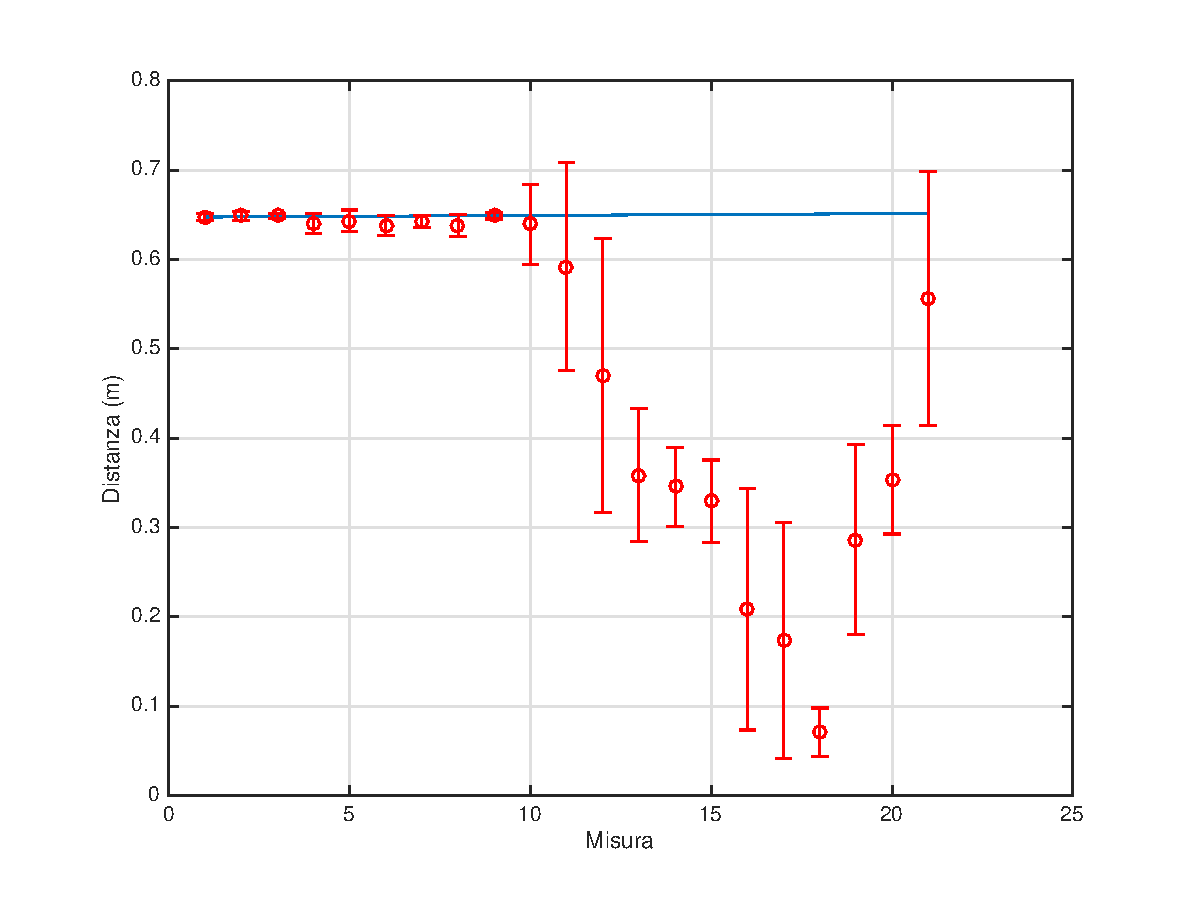
\includegraphics[scale=.5]{cap5/mismobile1}}
\hspace{5mm}
\subfigure[con finestra di Hanning]
{\label{mismobile2}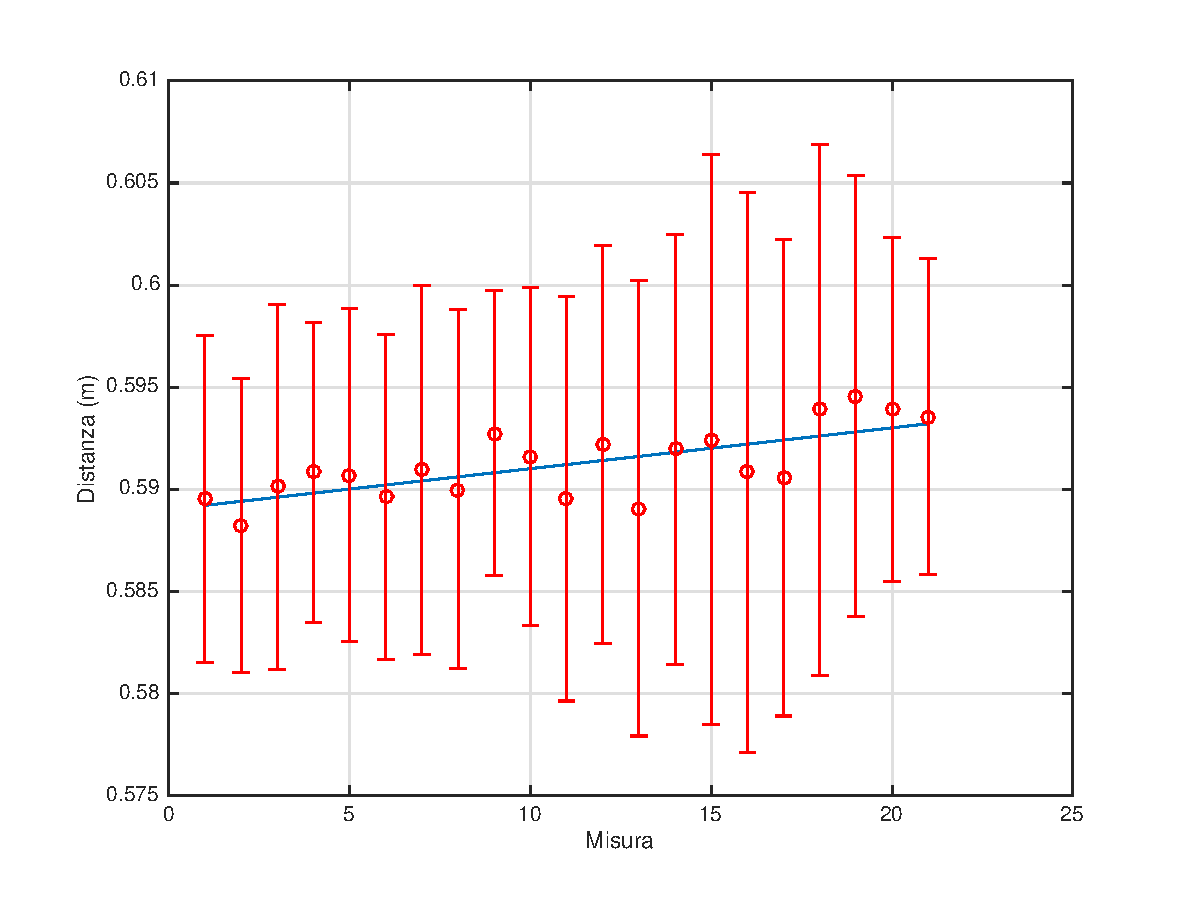
\includegraphics[scale=.5]{cap5/mismobile2}}
\caption{Misure di distanza a bersaglio mobile effettuate su $200 \mu m$ di spostamento}\label{mismobile12}
\end{figure}

I risultati delle prove a bersaglio fisso sono mostrati in Figura \ref{misfisso1} e \ref{misfisso2}. Sono inoltre riportati i grafici della distribuzione dei punti misurati rispetto alla media. In Figura \ref{mismobile12}, invece, sono mostrate le misure a bersaglio mobile: i punti rossi rappresentano le medie valutate ogni $100$ misurazioni, e le barre di errore mostrano l'incertezza assoluta di misura. La curva blu, invece, rappresenta il valore atteso.

Dai risultati delle misure a bersaglio fisso si evince che con la finestratura di \textit{Hanning} vi è un chiaro miglioramento in termini di precisione. L'incertezza relativa di misura si riduce complessivamente di un fattore $10$ passando da $10^{-1}$, con finestra rettangolare, a $10^{-2}$ con finestra di \textit{Hanning}.

Si nota inoltre, dai risultati delle misure a bersaglio mobile, che l'utilizzo della finestra di \textit{Hanning} rende lo strumento lineare allo spostamento con un errore massimo picco-picco dell'ordine del millimetro (ca. $4mm$). \'E facile intuire graficamente che l'utilizzo della finestra rettangolare rende lo strumento fortemente non lineare allo spostamento.
\begin{figure}  
  \begin{center}
    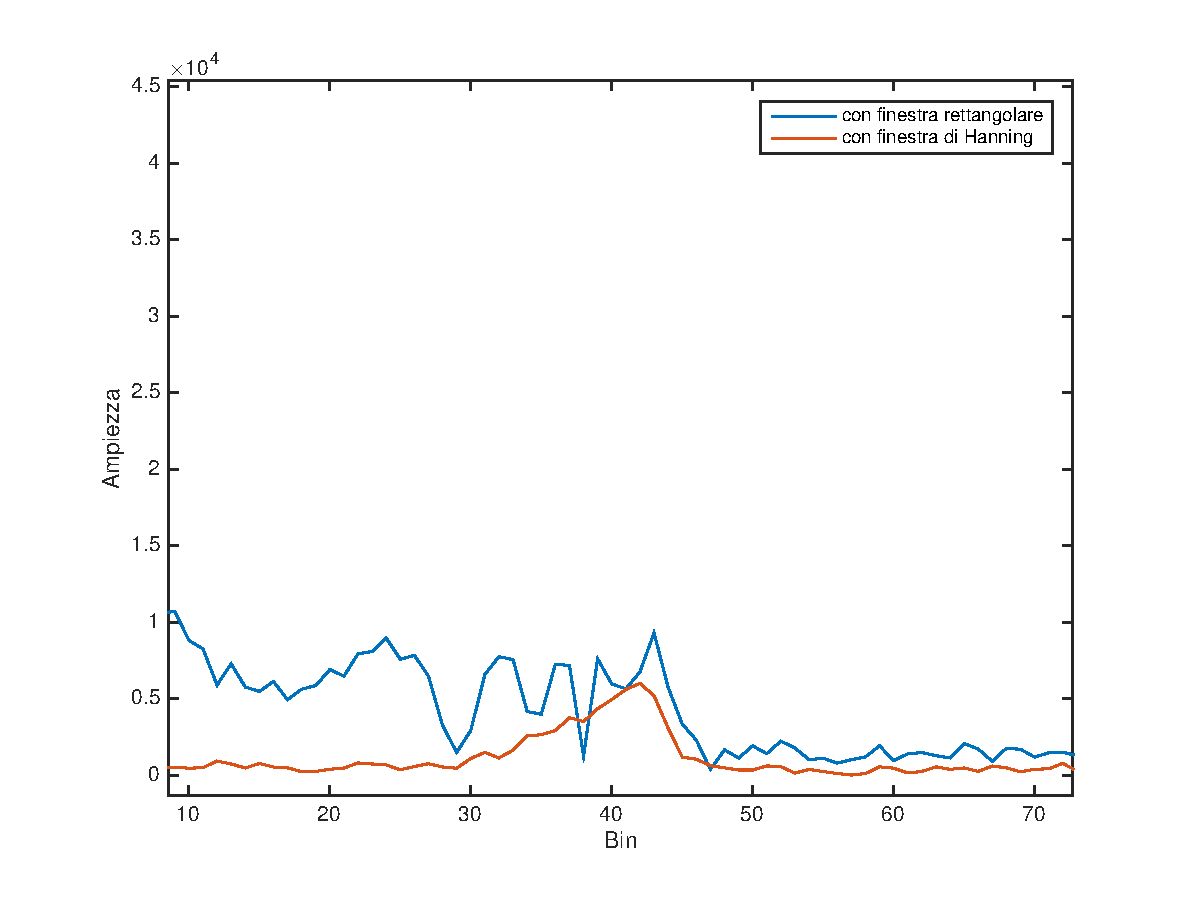
\includegraphics[scale=0.5]{cap5/spectleakinterf}
    \caption{Porzione di spettro calcolato sul fronte di discesa dalla FFT con finestra rettangolare e di Hanning}
    \label{spectleakinterf}
  \end{center}
\end{figure}

Il motivo che spiega questo miglioramento è la diminuzione dello \textit{spectral leakage}, che risulta meno marcato per la finestra di \textit{Hanning} piuttosto che per quella rettangolare. In Figura \ref{spectleakinterf} sono confrontati gli spettri di frequenza di un segnale interferometrico calcolati sul fronte di discesa dalla FFT con finestra rettangolare e di \textit{Hanning}. Dalla figura si nota l'evidente effetto dello \textit{spectral leakage} che affligge la FFT con finestra rettangolare.

\section{Linearizzazione della misura}
Nonostante i notevoli miglioramenti in termini di precisione, il misuratore possiede ancora una scarsa accuratezza. Tale limitazione dipende dalla lunghezza del periodo di frangia del segnale interferometrico. In particolare, fissata la distanza $s$ dell'ostacolo e modulando triangolarmente il laser, quindi con pendenza $\frac{\Delta I}{\Delta t}$ costante, il periodo di frangia $t_{frangia}$ dovrebbe essere costante lungo tutto il segnale. 
\begin{figure}  
  \begin{center}
    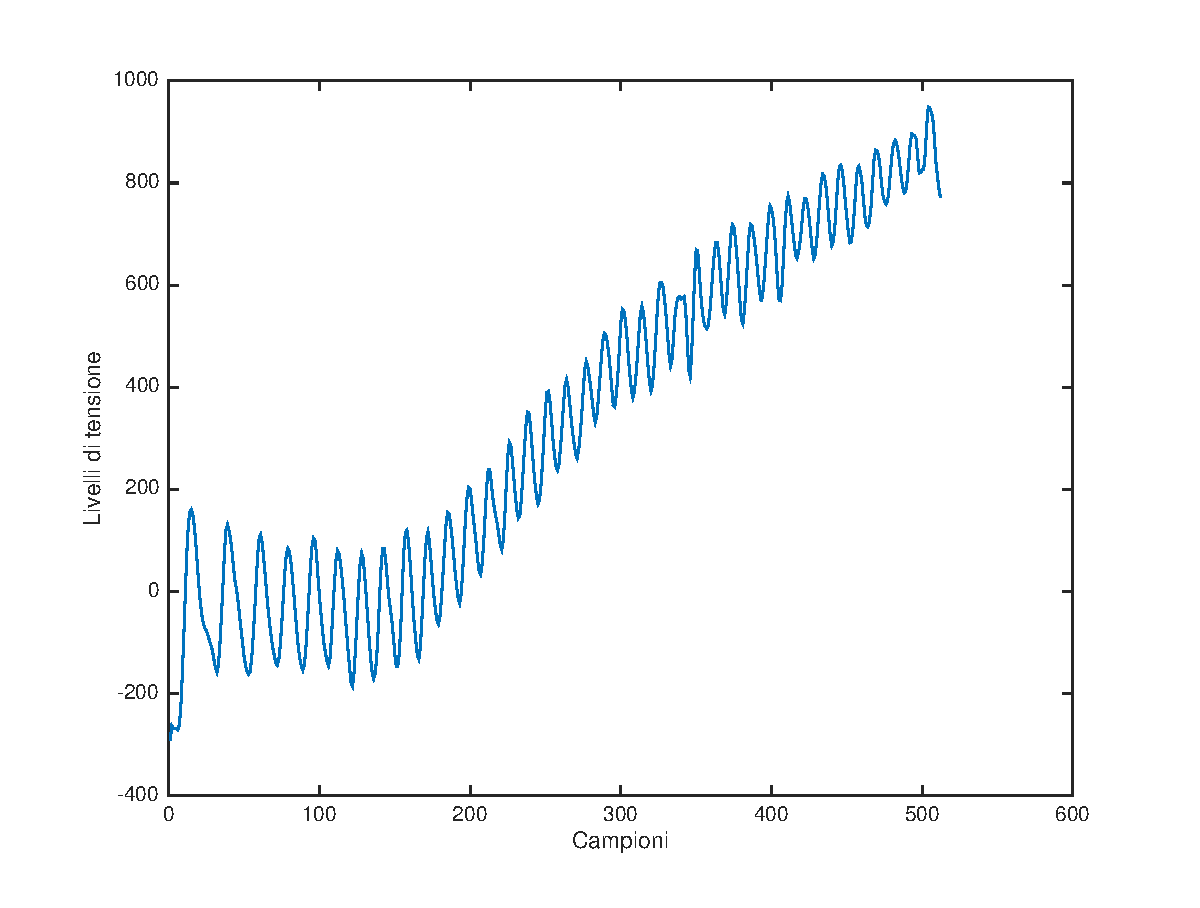
\includegraphics[scale=0.5]{cap5/semiperiodononcomp}
    \caption{Semiperiodo del segnale interferometrico prodotto dalla sorgente laser con modulazione a pendenza $\frac{\Delta I}{\Delta t}$ costante su di un bersaglio metallico a distanza fissa}
    \label{semiperiodononcomp}
  \end{center}
\end{figure}

Tuttavia, come osservato in Figura \ref{semiperiodononcomp}, il periodo della singola frangia $t_{frangia}$ non è costante lungo tutto il fronte di salita o di discesa. Di conseguenza, questo fenomeno è la causa del limite sull'accuratezza della misura.

Questo limite sull'accuratezza è dovuto alla non-linearità del laser. \'E possibile notare dall'equazione utilizzata per il calcolo della distanza assoluta: 
\begin{equation}
	s = \frac{\lambda^2}{2\left ( \frac{\Delta I}{\Delta t} \frac{\Delta \lambda}{\Delta I} \right ) t_{frangia}} 
\end{equation}
che è il parametro $\chi = \frac{\Delta \lambda}{\Delta I}$ a causare la non-linearità del periodo di frangia. Infatti dal momento in cui tutti i parametri sono fissati, l'unico che può causare la non-linearità è appunto $\chi$.

Un secondo motivo per cui il tempo di frangia $t_{frangia}$ non è costante è la costante termica del laser, che causa un ritardo nel raggiungimento di una condizione di equilibrio.

Queste caratteristiche sono peculiari della sorgente, e sono esclusivamente dipendenti dalla frequenza di modulazione della corrente.	

I due effetti combinati, quindi, causano una non linearità nella frequenza delle frange; in particolare le frange che si trovano all'inizio del segnale interferometrico sono a frequenza più bassa di quelle alla fine.	

\subsection{Metodo di compensazione della non-linearità}
\label{subsec:metodocomp}
Una tecnica per compensare le variazioni del parametro $\chi = \frac{\Delta \lambda}{\Delta I}$ consiste nell'utilizzare un segnale modulante con pendenza $\frac{\Delta I}{\Delta t}$ variabile durante il semiperiodo di modulazione. Per fare ciò è necessario ricavare l'andamento $\chi = \frac{\Delta \lambda}{\Delta I}$ conoscendo quello del $t_{frangia}$ o, in alternativa, $f_{frangia}$. Una volta ricavato l'andamento non-lineare nel tempo di $\chi = \frac{\Delta \lambda}{\Delta I}$ lo si compensa, modificando $\frac{\Delta I}{\Delta t}$, in modo che il prodotto $\frac{\Delta I}{\Delta t} \frac{\Delta \lambda}{\Delta I}$ sia costante e, di conseguenza, anche $t_{frangia}$ risulti costante.

Il metodo utilizzato per ricavare la forma d'onda del segnale di modulazione è stato implementato in LabVIEW Real-Time ed eseguito sul microprocessore della scheda di prototipazione. Per permettere ciò, è stato sviluppato un firmware FPGA, leggermente diverso de quello implementato nello strumento finale, che permettesse di inviare al microprocessore il segnale interferometrico completo e non solo i risultati dell'algoritmo di FFT.

Di seguito vengono descritti i passi principali del metodo di compensazione sviluppato:
\begin{figure}  
  \begin{center}
    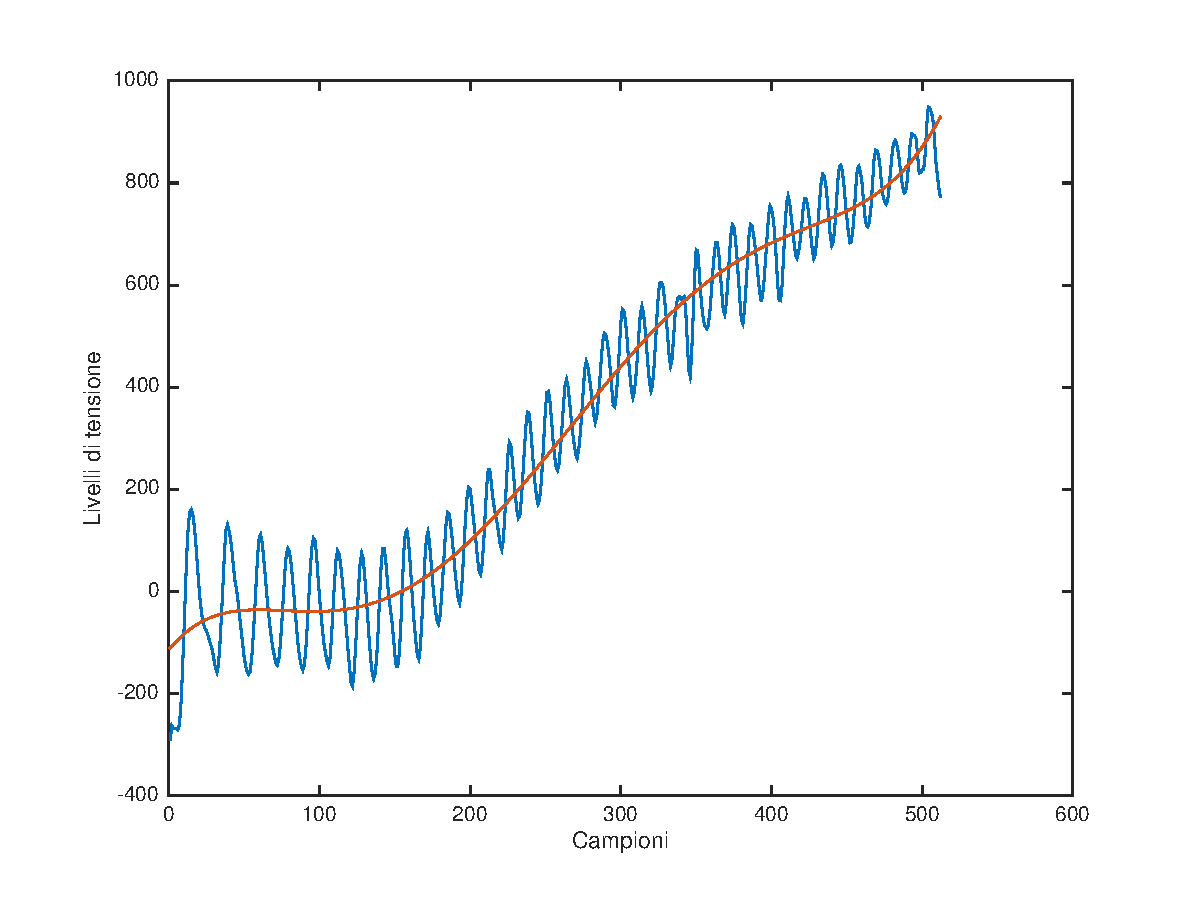
\includegraphics[scale=0.5]{cap5/regressioncurvefrangia}
    \caption{Curva di regressione polinomiale del segnale interferometrico}
    \label{regressioncurvefrangia}
  \end{center}
\end{figure}

\begin{figure}  
  \begin{center}
    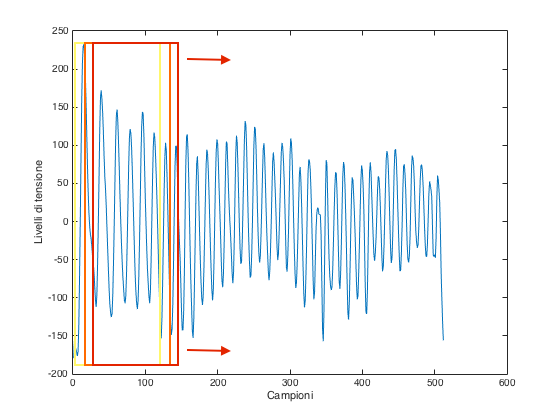
\includegraphics[scale=0.5]{cap5/slidingfft}
    \caption{Spostamento della finestra di 128 campioni lungo il semiperiodo di modulazione su cui viene calcolata la FFT}
    \label{slidingfft}
  \end{center}
\end{figure}

\begin{figure}  
  \begin{center}
    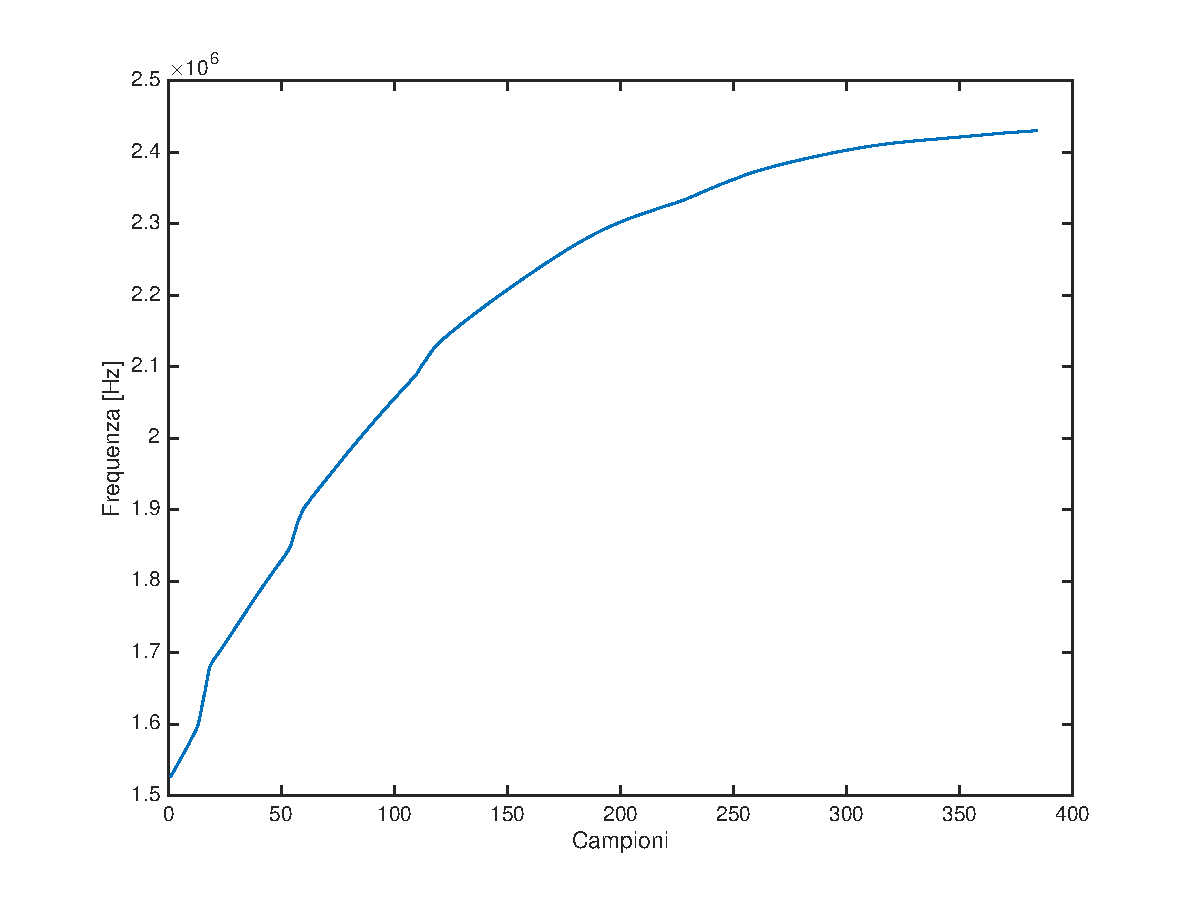
\includegraphics[scale=0.5]{cap5/curvamediatafreq}
    \caption{Curva mediata delle frequenze in un semiperiodo di modulazione con ostacolo a distanza fissa}
    \label{curvamediatafreq}
  \end{center}
\end{figure}

\begin{figure}
\centering
\subfigure[Semiperiodo di discesa]
{\label{}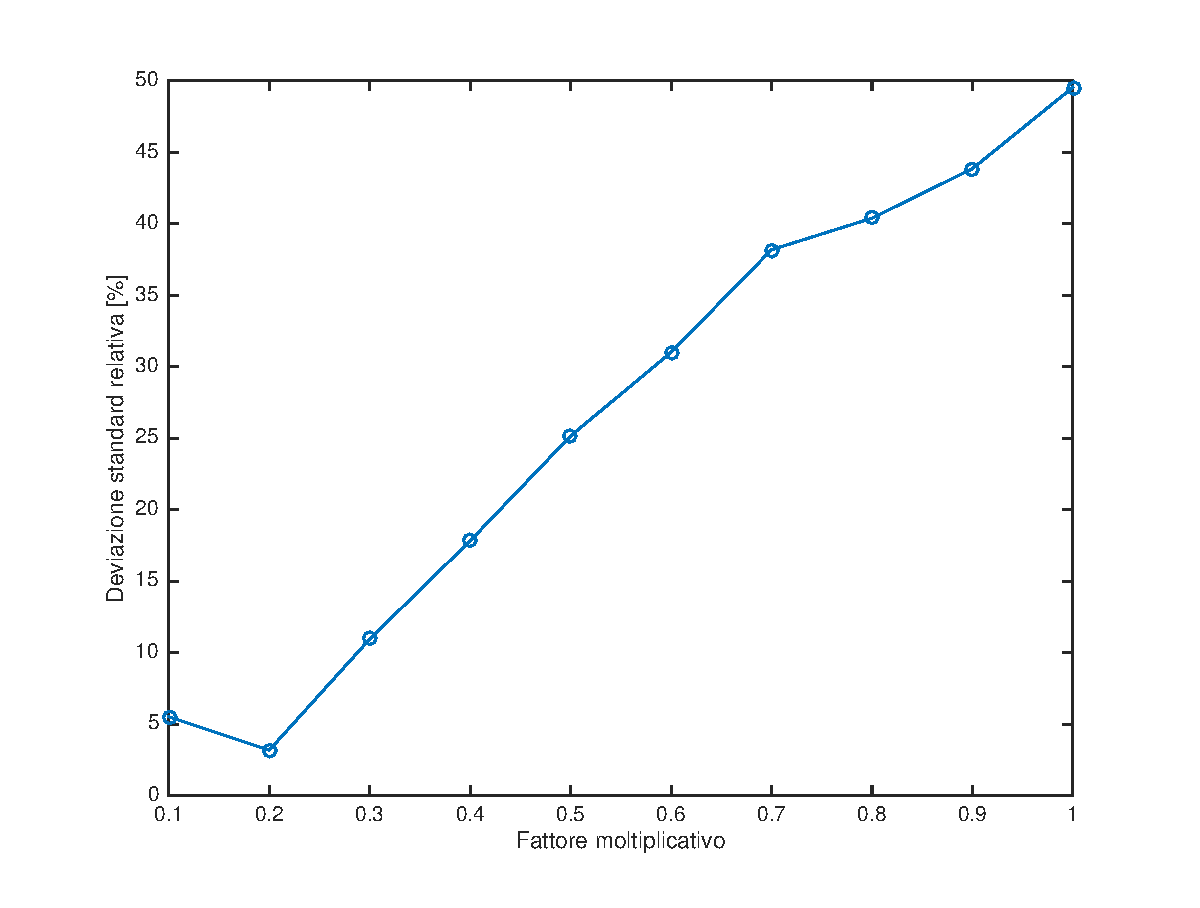
\includegraphics[scale=.3]{cap5/mulfactdiscesa}}
\hspace{5mm}
\subfigure[Semiperiodo di salita]
{\label{}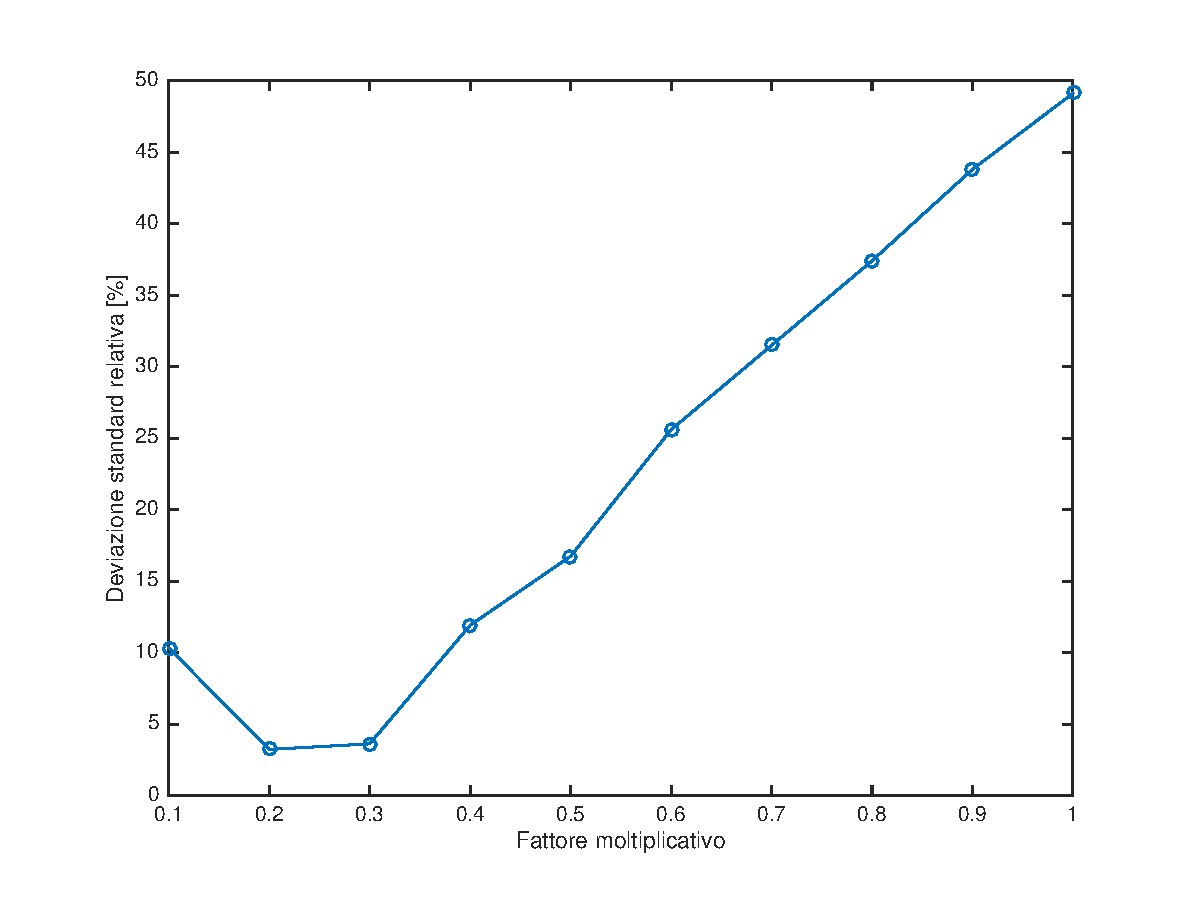
\includegraphics[scale=.3]{cap5/mulfactsalita}}
\caption{Curva delle deviazioni standard relative dei due fronti al variare del fattore moltiplicativo}\label{mulfact}
\end{figure}

\begin{enumerate}
	\item \underline{Modulazione triangolare}: La forma d'onda utilizzata per la modulazione è un'onda triangolare simmetrica con pendenza fissa. Il bersaglio è posto ad un distanza tale da produrre un elevato numero di frange (nel nostro caso si è posto il bersaglio a circa $50cm$ dal sensore).
	\item \underline{Calcolo della curva di regressione polinomiale}: Per avere una misura più precisa delle frequenza di frangia è stata calcolata la curva di regressione polinomiale di grado $5$ del segnale interferometrico (esempio in Figura \ref{regressioncurvefrangia}) ed è stata sottratta digitalmente da esso. In questo modo la lunghezza del tempo di frangia è valutata in modo più rigoroso.
	\item \underline{Calcolo della curva delle variazioni delle frequenze di frangia}: L'algoritmo analizza separatamente i due fronti, ricevendo in ingresso i $512$ campioni del segnale interferometrico per ciascun fronte. Per ogni fronte si selezionano i primi $128$ campioni e si estrae il valore di frequenza corrispondente alle prime frange del segnale. Per l'estrazione della frequenza del segnale, LabVIEW offre un metodo già implementato chiamato \textit{Extract Single Tone Information}. Si tratta di una FFT con finestra di \textit{Hanning} interpolata a due punti, con una correzione per l'aliasing intorno alla continua a $\frac{f_{sample}}{2}$. A questo punto la finestra di selezione viene traslata di un campione verso destra e la frequenza delle frange viene ricalcolata (Figura \ref{slidingfft}). Questa operazione viene effettuata fino a che la selezione comprende l'ultimo campione del segnale interferometrico.
	
	In questo modo si ottengono $384$ valori di frequenze per ciascun fronte, in funzione della posizione delle frange all'interno del fronte stesso (Figura \ref{curvamediatafreq}). Questo procedimento è stato effettuato per $100$ segnali acquisiti ed i risultati sono stati poi mediati. \'E stato deciso di associare ai primi $113$ ($=625-512$) campioni scartati valori di frequenza fittizi, approssimando tali valori con una retta di pendenza pari alla pendenza della prima frequenza estratta, mentre agli ultimi $128$ ($=512-384$) campioni è stata associata una retta con pendenza pari alla pendenza dell'ultima frequenza estratta.
	\item \underline{Calcolo iterativo del fattore moltiplicativo} \underline{da applicare alla curva delle} \underline{frequenze}: La curva mediata delle frequenze, ricavata al passo precedente, viene moltiplicata alla triangolare con pendenza costante ricavando così il segnale di modulazione con pendenza $\frac{\Delta I}{\Delta t}$ non costante.
	
	Da verifiche sperimentali è nata la necessità di moltiplicare i semiperiodi della curva di modulazione per un fattore di scala, che è stato scelto in modo che la deviazione standard relativa delle frequenze rilevate dall'FFT a scorrimento sia la minore possibile.
	
	Questo fattore viene ricavato iterativamente. Partendo da un valore $1$ e diminuendo il fattore di scala di passi di $0.1$ fino ad arrivare a $0$, si calcola la deviazione standard relativa delle frequenze estratte dall'FFT a scorrimento e si sceglie il fattore di scala che la minimizza.
	
	Questo procedimento è stato reiterato una seconda volta aumentando il numero di cifre significative del fattore di scala stesso (partendo da $0.35$ ed arrivando a $0.15$ con passi di $0.01$), in modo da aumentare la precisione della linearizzazione.
	
	Le prime curve ricavate vengono presentate in Figura \ref{mulfact}. Si può notare che sia per il fronte di salita che per il fronte di discesa il minimo si trova nell'intorno di $0.2$. I valori esatti ricavati nella seconda iterazione sono $0.18$ per il fronte di discesa e $0.22$ per il fronte di salita.
	\item \underline{Generazione della curva di modulazione compensata}: Le curve delle variazioni delle frequenze di frangia, calcolate al passo 2, vengono scalate dei valori moltiplicativi calcolati al passo precedente. Le curve scalate vengono poi moltiplicate ai semiperiodi della triangolare con pendenza costante ricavando così il segnale di modulazione con pendenza $\frac{\Delta I}{\Delta t}$ non costante.	
\end{enumerate}
\begin{figure}  
  \begin{center}
    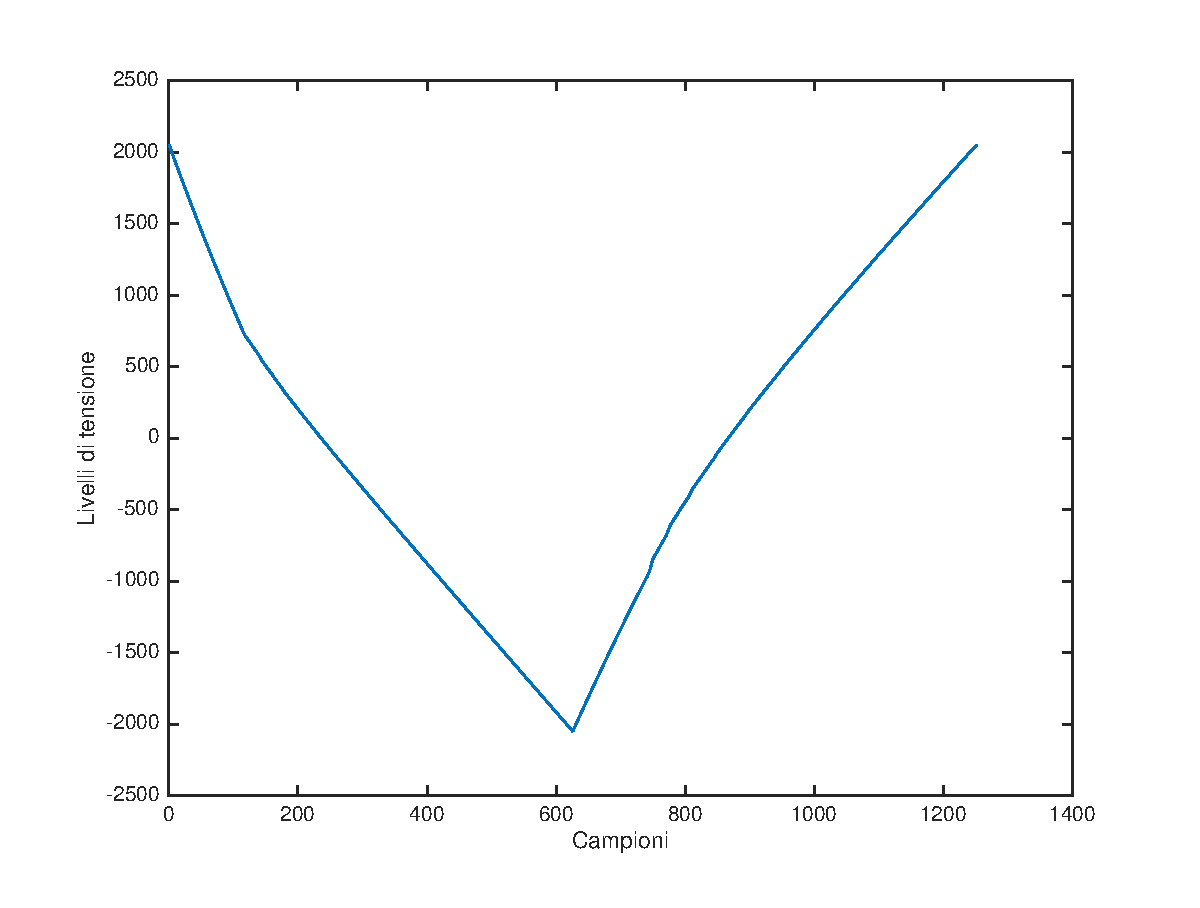
\includegraphics[scale=0.5]{cap5/ondafinale}
    \caption{Forma d'onda finale usata per la modulazione}
    \label{ondafinale}
  \end{center}
\end{figure}

La forma d'onda finale, mostrata in Figura \ref{ondafinale}, ha consentito di ridurre la dispersione del $t_{frangia}$, migliorando l'accuratezza della misura di distanza. La pendenza iniziale sia nel fronte di salita che in quello di discesa è accentuata rispetto alla triangolare originaria, come era prevedibile dallo studio in frequenza. Infatti la frequenza di frangia presentava un andamento monotono crescente al variare della corrente di modulazione, effetto compensato dall'aumento della pendenza nella triangolare compensata.

\subsection{Misure in seguito alla compensazione}
Al fine di valutare la bontà dell'algoritmo precedentemente descritto, è stata comparata quantitativamente l'incertezza relativa della variazione di frequenza del segnale interferometrico prima e dopo la compensazione del segnale di modulazione.

\begin{figure}
\centering
\subfigure[Semiperiodo di discesa]
{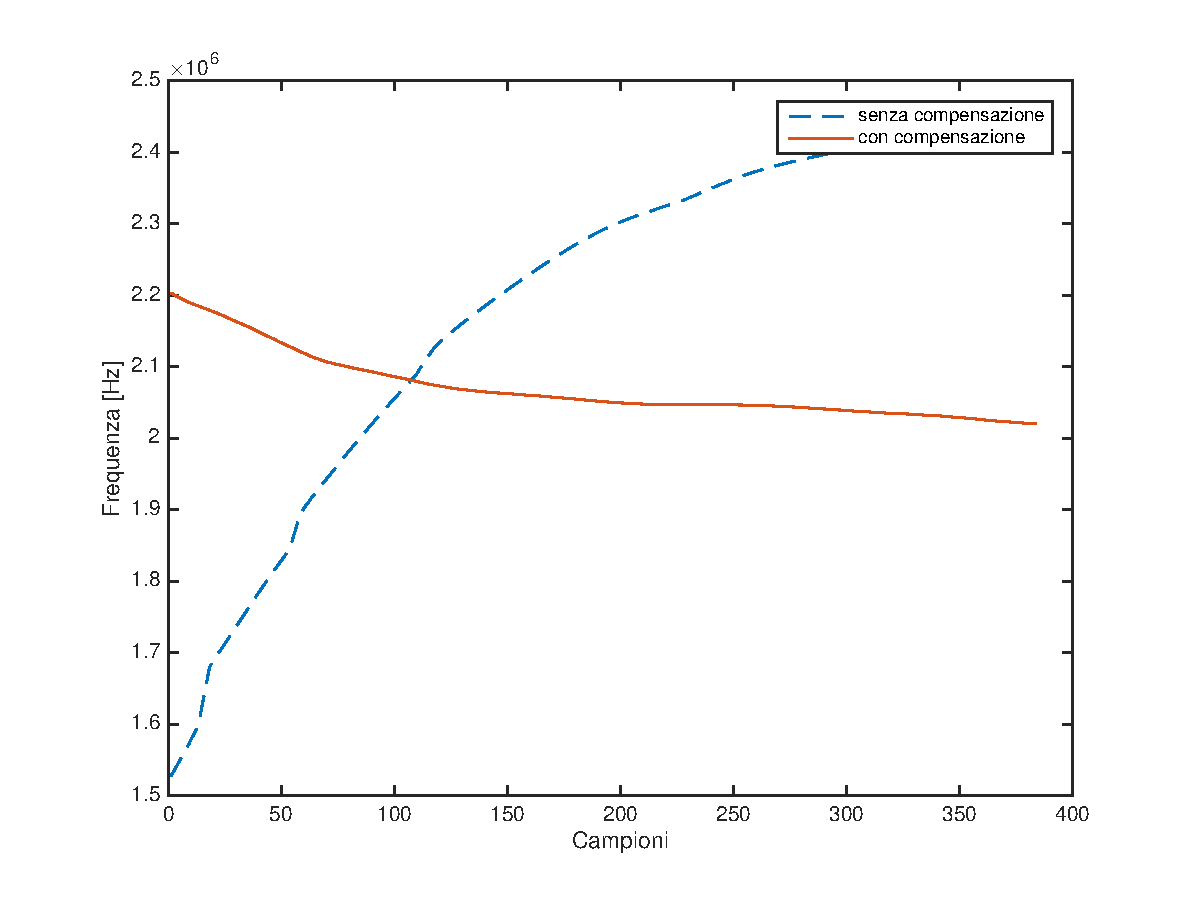
\includegraphics[scale=.3]{cap5/primadopocompdisc}}
\hspace{5mm}
\subfigure[Semiperiodo di salita]
{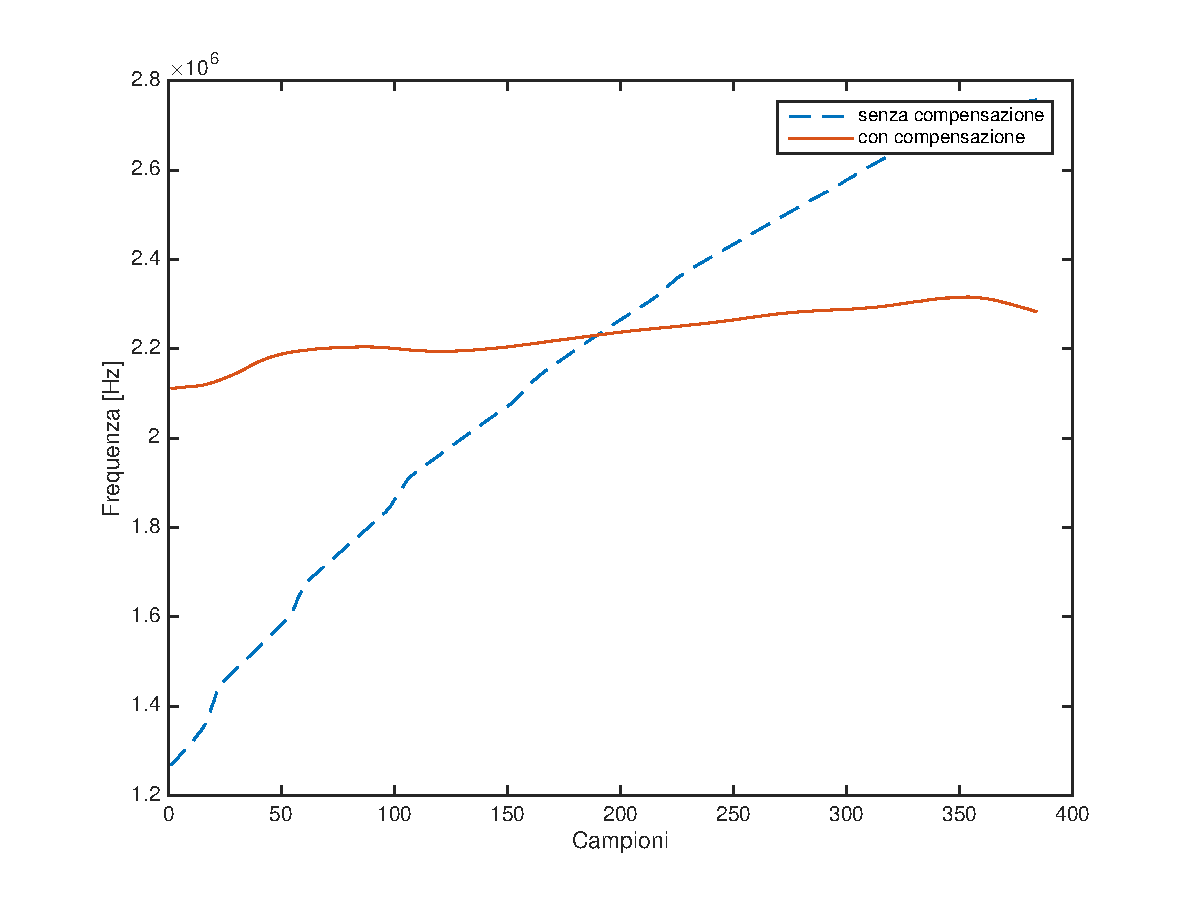
\includegraphics[scale=.3]{cap5/primadopocompsal}}
\caption{Curve mediate delle frequenze estratte per entrambi i fronti di modulazione, prima e dopo la compensazione}\label{primadopocomp}
\end{figure}

I miglioramenti ottenuti per merito della compensazione della non-linearità sono mostrati in Figura \ref{primadopocomp}. Dalle prove sperimentali è emerso che l'incertezza relativa della variazione di frequenza, valutata su $100$ semiperiodi di modulazione, è scesa intorno al $2\%$, per entrambi i fronti di modulazione, contro i $20\%$ ottenuti senza compensazione. La prova è stata ripetuta più volte per verificare che il guadagno in termini di linearità del periodo di frangia sia effettivamente $10$.
\begin{figure}
\centering
\subfigure[Misure di distanza e media]
{\label{misfisso3a}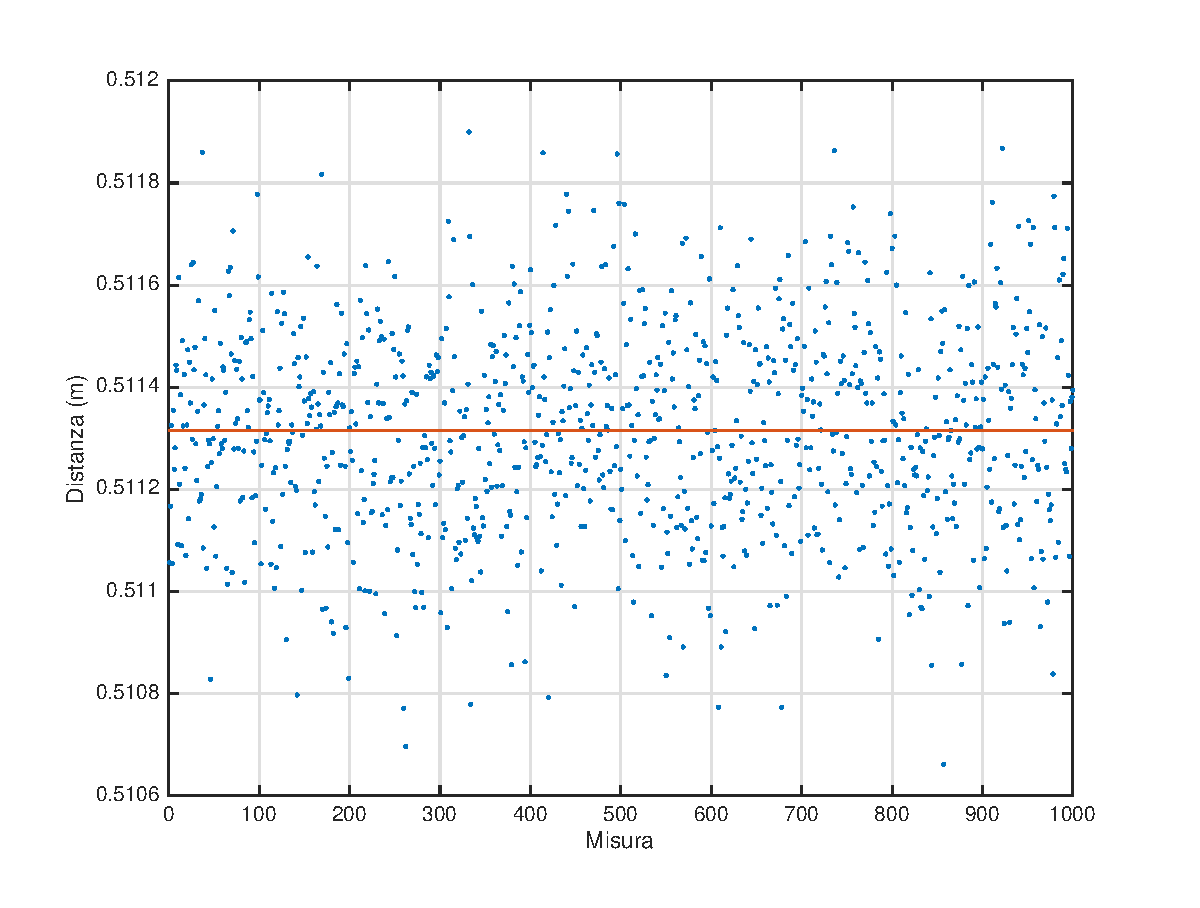
\includegraphics[scale=.5]{cap5/misfisso3a}}
\hspace{5mm}
\subfigure[Distribuzione dei valori misurati rispetto alla media]
{\label{misfisso3b}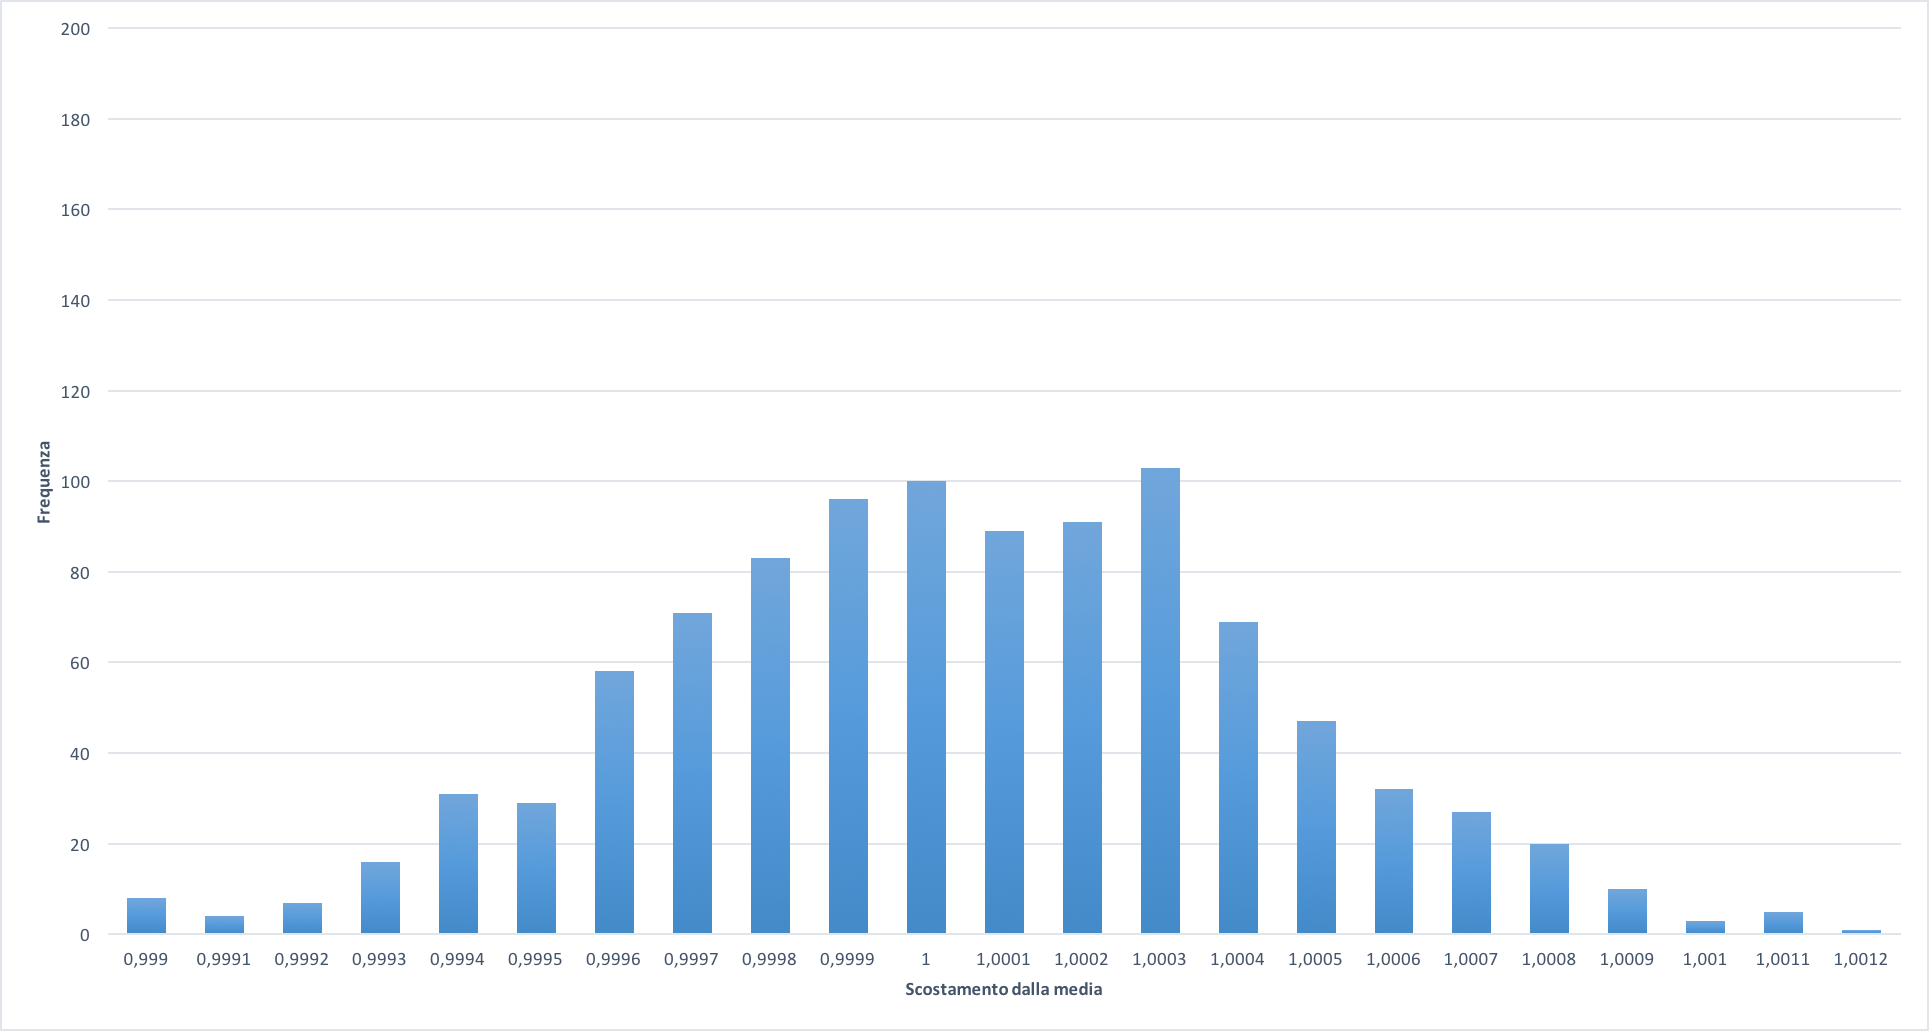
\includegraphics[scale=.35]{cap5/misfisso3b}}
\caption{Misure a bersaglio fisso con segnale di modulazione compensato}\label{misfisso3}
\end{figure}

\begin{figure}  
  \begin{center}
    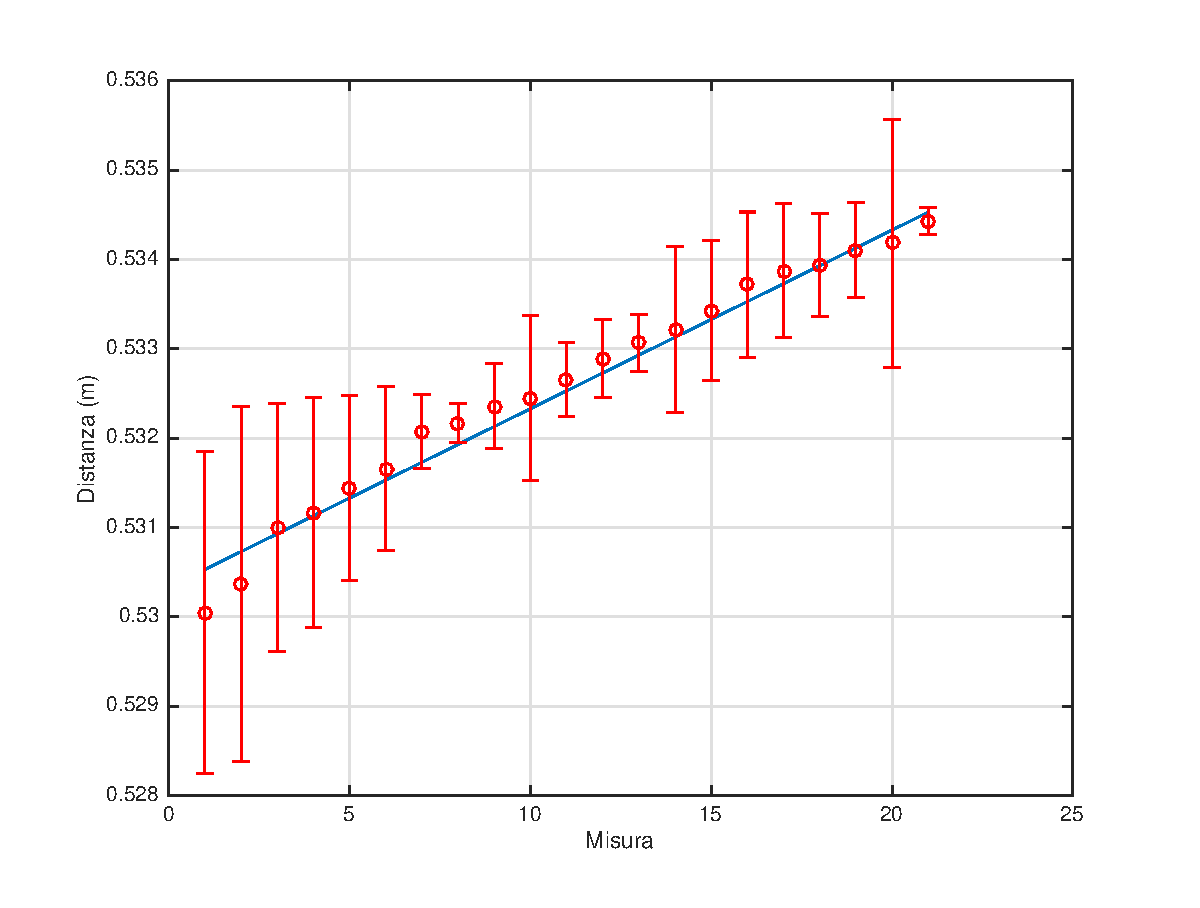
\includegraphics[scale=0.5]{cap5/mismobile3}
    \caption{Misure di distanza a bersaglio mobile effettuate su $200\mu m$ di spostamento con segnale di modulazione compensato}
    \label{mismobile3}
  \end{center}
\end{figure}

Questo miglioramento ha influito sulla precisione e sull'accuratezza della misura. A conferma del risultato sono riportati gli esiti delle prove a bersaglio fisso e a bersaglio mobile rispettivamente in Figura \ref{misfisso3} e \ref{mismobile3}.

Si può apprezzare, dai risultati delle misure a bersaglio fisso, che utilizzando un segnale di modulazione compensato la precisione di misura migliora sensibilmente. In particolare, l'incertezza relativa diminuisce di due ordini di grandezza, passando da $10^{-2}$ a $4 \cdot 10^{-4}$.

Inoltre, si può notare come le misure effettuate con la modulazione compensata risultino complessivamente più lineari rispetto a quelle effettuate senza compensazione.

La valutazione dell'errore massimo picco-picco rispetto al valore atteso conferma quanto intuito graficamente: l'errore nel caso di segnale di modulazione con pendenza compensata migliora considerevolmente passando da $4mm$ a $826 \mu m$, con un RMS pari a $568 \mu m$.

Nonostante l'ottimo miglioramento raggiunto, l'accuratezza non è ancora soddisfacente, a tal proposito si è ritenuto opportuno migliorare ulteriormente la misura con ottimizzazioni che verranno descritte nel paragrafo successivo.

\section{Ottimizzazione della misura}
In questo paragrafo verranno discusse le ottimizzazioni sviluppate al fine di migliorare la precisione e l'accuratezza della misura.

\subsection{Variazione dell'ampiezza del segnale di modulazione}
\begin{figure}  
  \begin{center}
    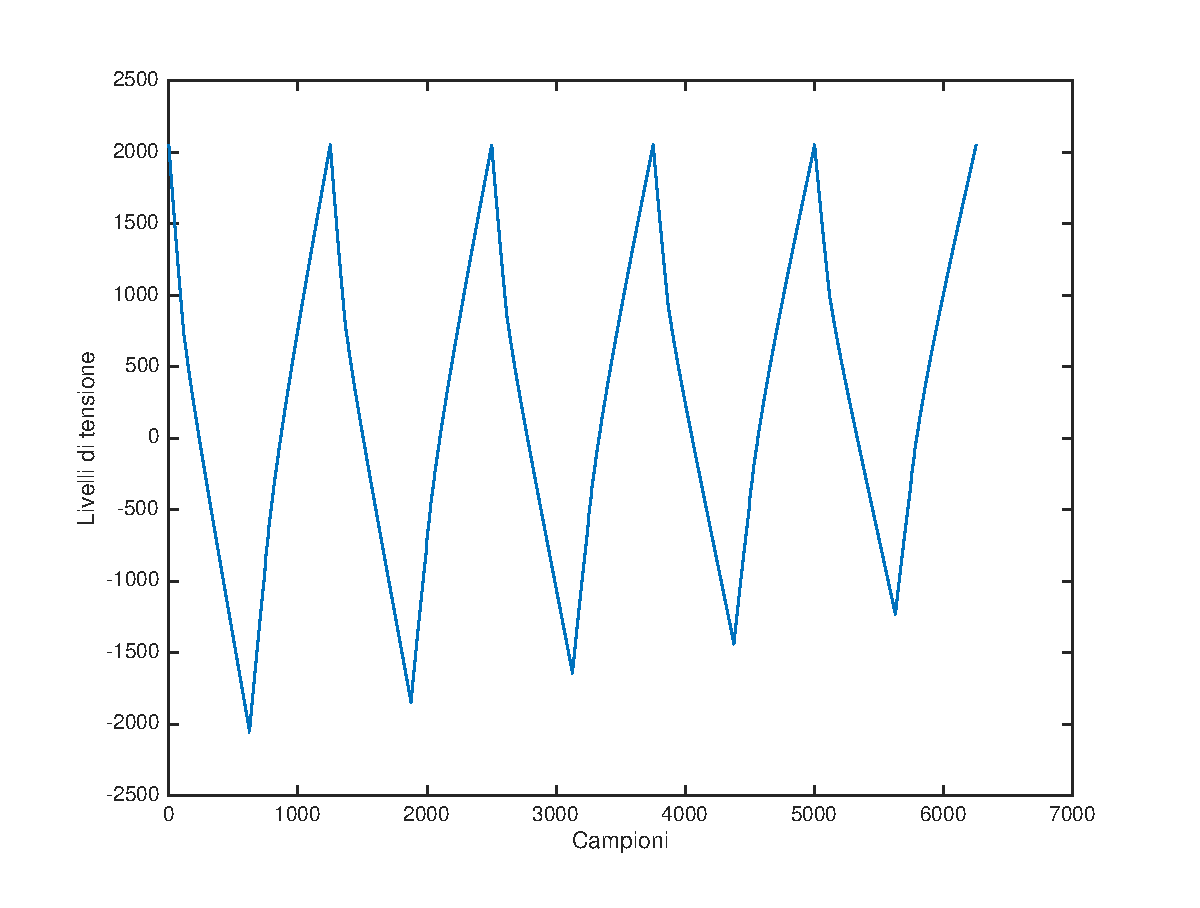
\includegraphics[scale=0.5]{cap5/cinquesegnali}
    \caption{Segnale di modulazione compensato, costituito da cinque forme d'onda di ampiezza diversa}
    \label{cinquesegnali}
  \end{center}
\end{figure}

Per cercare di mitigare effetti dipendenti dall'ampiezza del segnale di modulazione sul laser si è deciso di utilizzare un segnale di modulazione ad ampiezza variabile. Poiché le prestazioni dello strumento in termini di velocità di acquisizione di una singola misura sono piuttosto elevate (il tempo di misura teorico è di circa $40 \mu s$), si è deciso di utilizzare $5$ segnali di modulazione con ampiezze differenti (Figura \ref{cinquesegnali}). Le ampiezze scelte per i segnali sono state rispettivamente di $100\%$, $95\%$, $90\%$, $85\%$ e $80\%$ rispetto al segnale di modulazione utilizzato inizialmente.	

Diverse ampiezze del segnale di modulazione restituiscono frequenze di interferenza diverse a parità di distanza del sensore dal bersaglio.

Questo fenomeno è facilmente verificabile osservando la consueta formula per il calcolo della distanza assoluta:
\begin{equation}
	s = \frac{\lambda^2}{2\left ( \frac{\Delta I}{\Delta t} \frac{\Delta \lambda}{\Delta I} \right )}  f_{frangia} 
\end{equation}

Poiché variando le ampiezze dei segnali di modulazione varia il valore di $\frac{\Delta I}{\Delta t}$, mentre gli altri elementi dell'equazione restano costanti. \'E facile dimostrare che all'aumentare dell'ampiezza del segnale di modulazione e a parità di distanza aumenta la frequenza di frangia $f_{frangia}$.
\begin{table}[]
\centering
\begin{tabular}{l|l|l|}
\multirow{3}{*}{\textbf{\begin{tabular}[c]{@{}l@{}}Fattore moltiplicativo\\ del segnale di\\ modulazione {[}\%{]}\end{tabular}}} & \multicolumn{2}{c|}{\multirow{2}{*}{\textbf{Fattore di correzione della frequenza}}} \\
 & \multicolumn{2}{c|}{} \\ \cline{2-3} 
 & \textbf{di discesa {[}\%{]}} & \multicolumn{1}{l|}{\textbf{di salita {[}\%{]}}} \\ \hline
\textbf{80} & 77.8805 & 88.0774 \\
\textbf{85} & 83.9557 & 92.338 \\
\textbf{90} & 90.3068 & 96.5311 \\
\textbf{95} & 95.8657 & 100.965 \\
\textbf{100} & \textbf{100} & 105.502
\end{tabular}
\caption{Fattori correttivi di frequenza}
\label{tabfattoricorr}
\end{table}

Per questo motivo tutte le frequenze misurate sono riportate al valore, ritenuto nominale, del semiperiodo di discesa con ampiezza $100\%$. Questa operazione fa si che le distanze misurate con le diverse ampiezze di modulazione siano tra loro comparabili. I valori di correzione di frequenza sono mostrati in Tabella \ref{tabfattoricorr}.

Si può notare un leggero scostamento tra i fattori correttivi empirici e i valori teorici. Ciò accade in quanto, con la variazione del parametro $\frac{\Delta I}{\Delta t}$, la linearizzazione del parametro $\frac{\Delta \lambda}{\Delta I}$ non avviene più in maniera rigorosa.
\begin{figure}  
  \begin{center}
    \includegraphics[scale=0.52]{cap5/cinquesegnalidis}
    \caption{Segnale di modulazione compensato, costituito da cinque forme d'onda di ampiezza diversa in ordine sparso}
    \label{cinquesegnalidis}
  \end{center}
\end{figure}

L'utilizzo di segnali differenti con ampiezze in ordine decrescente può portare alla creazione di un trend nel segnale di modulazione, causato dall'andamento crescente dei picchi negativi dei segnali. Questo può causare un degrado delle prestazioni della misura, per questo si è deciso di alternare le differenti ampiezze del segnale in modo che l'andamento dei picchi sia il meno deterministico possibile (Figura \ref{cinquesegnalidis}).

L'utilizzo di questa tecnica peggiora il tempo di acquisizione di una singola misura, in quanto, ora, un singolo valore di distanza è ottenuto dalla media dei $5$ valori ricavati utilizzando i $5$ segnali con ampiezze differenti.

Questo approccio, tuttavia, permette di scorrelare l'errore di misura provocato dallo sfasamento iniziale delle frange, permettendo una riduzione teorica di $\sqrt{5}$ sulla deviazione standard della misura. 

Tramite la prova a bersaglio fisso si è notato un miglioramento della deviazione standard di un fattore $2$, leggermente minore del risultato teorico atteso ($\sqrt{5} \approx 2.24$). La deviazione standard relativa su $1000$ misure effettuate ad una distanza di $50 cm$ dal bersaglio è passata da $4 \cdot 10^{-4}$ a $2.5 \cdot 10^{-4}$. 

\begin{figure}
\centering
\subfigure[Misure di distanza e media]
{\label{misfisso4a}\includegraphics[scale=.5]{cap5/misfisso4a}}
\hspace{5mm}
\subfigure[Distribuzione dei valori misurati rispetto alla media]
{\label{misfisso4b}\includegraphics[scale=.3]{cap5/misfisso4b}}
\caption{Misure a bersaglio fisso con i 5 segnali di modulazione}\label{misfisso4}
\end{figure}

\begin{figure}  
  \begin{center}
    \includegraphics[scale=0.5]{cap5/mismobile4}
    \caption{Misure di distanza a bersaglio mobile effettuate su $200\mu m$ di spostamento con i 5 segnali di modulazione}
    \label{mismobile4}
  \end{center}
\end{figure}

L'introduzione di questa tecnica migliora anche la linearità dello strumento, come è chiaramente verificabile attraverso la prova a bersaglio mobile (Figura \ref{mismobile4}).

L'errore picco-picco misurato con questa prova è di $451 \mu m$, mentre l'RMS è $142 \mu m$.

Rispetto al caso precedente l'errore picco picco diminuisce di un fattore $2$, mentre l'RMS dell'errore rispetto alla retta ideale migliora di un fattore $5$.

\subsection{Sottrazione del residuo}
Come già trattato nei capitoli precedenti, l'algoritmo usato per calcolare l'FFT interpolata a 2 punti con finestra di \textit{Hanning} fa uso del bin di ampiezza massima e del bin di ampiezza maggiore scelto tra il precedente ed il successivo.

Analizzando il segnale in arrivo dal sensore laser in assenza di ostacolo, si è notata la presenza di un residuo causato dallo sottrazione non perfetta presente nello stadio analogico. Tale residuo è un errore deterministico che può influenzare negativamente la scelta del bin laterale nella algoritmo di FFT interpolata, poiché nella maggior parte dei casi essi, rispetto al massimo bin, avranno ampiezze relativamente basse e comparabili al segnale contenuto nel residuo. Questo può portare ad un errore nella stima del bin interpolato e quindi influenzare negativamente la precisione della misura.

Per cercare di mitigare l'effetto del rumore deterministico causato dal residuo si è deciso di procedere sottraendo al segnale interferometrico acquisito il suo residuo.

All'avvio dello strumento, con il sensore in assenza di ostacolo, si acquisiscono e mediano $1000$ segnali in assenza di frange. Il risultato della media è un segnale che chiamiamo "residuo". Perciò, per ogni successiva acquisizione di segnale interferometrico, si procede alla sottrazione del residuo al segnale acquisito.

La sottrazione è effettuata al momento dell'acquisizione del segnale, perciò le componenti del residuo sono sottratte sia in ampiezza che in frequenza. 

Utilizzando questa tecnica si è notato un miglioramento delle prestazioni dello strumento a basse frequenze. Ciò accade perché il residuo estratto è correlato al rumore della misura solo per determinate frequenze e la sottrazione del residuo su tutto lo spettro porta, per frequenze maggiori, all'aggiunta di ulteriore rumore alla misura.

Per mantenere i vantaggi della sottrazione del residuo a basse frequenze senza peggiorare la misura ad alte frequenze si è deciso di applicare un filtro passa-basso al residuo acquisito.

Sperimentalmente si è verificato che sottraendo il residuo per frequenze più basse di $1 \div 1.5MHz$ si ha un miglioramento della deviazione standard relativa della misura, mentre per frequenze più elevate la sottrazione del residuo porta ad un peggioramento della misura.
Per queste ragioni si è scelto in modo conservativo come frequenza di taglio del filtro passa-basso $1MHz$, per evitare di aggiungere ulteriore rumore alla misura.


\begin{table}[]
\centering
\begin{tabular}{c|l|l|}
\multicolumn{1}{l|}{} & \multicolumn{2}{c|}{\textbf{Deviazione standard relativa}} \\ \hline
\multicolumn{1}{l|}{\textbf{\begin{tabular}[c]{@{}l@{}}Frequenza \\ (Distanza)\end{tabular}}} & \textbf{con sottrazione del residuo} & \textbf{senza sottrazione} \\ \hline
\textbf{\begin{tabular}[c]{@{}c@{}}800 KHz\\ (ca. 20cm)\end{tabular}}  & $2 \cdot 10^{-4} \div 3 \cdot 10^{-4}$ & $3 \cdot 10^{-4} \div 4 \cdot 10^{-4}$   \\
\textbf{\begin{tabular}[c]{@{}c@{}}1.5 MHz\\ (ca. 40cm)\end{tabular}} & $4 \cdot 10^{-4} \div 5 \cdot 10^{-4}$  & $4 \cdot 10^{-4} \div 5 \cdot 10^{-4}$ \\
\textbf{\begin{tabular}[c]{@{}c@{}}3.5 MHz\\ (ca. 90cm)\end{tabular}} & $6 \cdot 10^{-4} \div 7 \cdot 10^{-4}$ & $5 \cdot 10^{-4} \div 6 \cdot 10^{-4}$
\end{tabular}
\caption{Valori sperimentali di deviazione standard relativa calcolati su $1000$ misure a ostacolo fisso}
\label{tab:residuofatt}
\end{table}

In Tabella \ref{tab:residuofatt} è mostrato il range di deviazioni standard relative misurate al variare della frequenza.
\begin{figure}  
  \begin{center}
    \includegraphics[scale=0.5]{cap5/residuo}
    \caption{Residuo filtrato passa-basso con frequenza di taglio a 1 MHz}
    \label{residuo}
  \end{center}
\end{figure}

Anche per queste implementazioni sono state eseguite le consuete prove descritte nei paragrafi precedenti.
\begin{figure}
\centering
\subfigure[Misure di distanza e media]
{\label{misfisso5a}\includegraphics[scale=.5]{cap5/misfisso5a}}
\hspace{5mm}
\subfigure[Distribuzione dei valori misurati rispetto alla media]
{\label{misfisso5b}\includegraphics[scale=.4]{cap5/misfisso5b}}
\caption{Misure di distanza a bersaglio fisso con sottrazione del residuo}\label{misfisso5}
\end{figure}

Nella prova a bersaglio fisso (Figura \ref{misfisso5}) si è notato un miglioramento non sostanziale rispetto al caso senza sottrazione del residuo. Questo accade a causa del posizionamento del bersaglio; infatti, alla distanza di $50 cm$, la frequenza misurata (ca. $1.9MHz$) è al di sopra della frequenza di taglio del filtro passa-basso che agisce sul residuo estratto, rendendo la sottrazione del residuo poco efficace.

In questo caso il valore di deviazione standard relativa calcolato su $1000$ campioni vale $2.4 \cdot 10^{-4}$.

Nella Figura \ref{misfisso5b} è stata sovrapposta la distribuzione gaussiana teorica dei valori, e si può notare che i dati empirici sono aderenti ad essa.

\begin{figure}  
  \begin{center}
    \includegraphics[scale=0.5]{cap5/mismobile5}
    \caption{Misure di distanza a bersaglio mobile con sottrazione del residuo effettuate su $200 \mu m$ di spostamento}
    \label{mismobile5}
  \end{center}
\end{figure}

Dai risultati ottenuti nella prova a bersaglio mobile (Figura \ref{mismobile5}) si ottiene, al contrario dell'esperimento a bersaglio fisso, un notevole miglioramento nell'accuratezza. Vi è un dimezzamento, rispetto al caso senza sottrazione del residuo, della distanza picco-picco dell'errore. Essa scende a $280 \mu m$ con un RMS pari a $124 \mu m$.

\section{Prove dello strumento finale}
Alla luce dei risultati riportati nei paragrafi precedenti, nell'implementazione finale dello strumento si è deciso di utilizzare l'algoritmo a $5$ segnali di modulazione con sottrazione del residuo.

Questa scelta è stata fatta poiché l'intervallo di misura garantito permette di avere precisioni migliori a basse distanze, senza avere peggioramenti significativi nella restante zona di funzionamento del sensore.

Come anticipato in precedenza con la configurazione finale sono state eseguite due ulteriori prove a bersaglio fisso e mobile alle distanze di $20cm$ e $90cm$, i cui risultati sono riportati di seguito.

\subsection{Bersaglio fisso}
\begin{figure}
\centering
\subfigure[Misure di distanza e media]
{\label{misfisso5a20}\includegraphics[scale=.5]{cap5/misfisso5a20}}
\hspace{5mm}
\subfigure[Distribuzione dei valori misurati rispetto alla media]
{\label{misfisso5b20}\includegraphics[scale=.4]{cap5/misfisso5b20}}
\caption{Misure di distanza a 20cm con bersaglio fisso }\label{misfisso520}
\end{figure}

\begin{figure}
\centering
\subfigure[Misure di distanza e media]
{\label{misfisso5a90}\includegraphics[scale=.5]{cap5/misfisso5a90}}
\hspace{5mm}
\subfigure[Distribuzione dei valori misurati rispetto alla media]
{\label{misfisso5b90}\includegraphics[scale=.4]{cap5/misfisso5b90}}
\caption{Misure di distanza a 90cm con bersaglio fisso }\label{misfisso590}
\end{figure}

Nella prova a bersaglio fisso a $20cm$ (Figura \ref{misfisso520}) si ottiene una deviazione standard relativa di $1.32 \cdot 10^{-4}$, mentre con il bersaglio a $90cm$  (Figura \ref{misfisso590}) la deviazione standard relativa ottenuta è di $6.5 \cdot 10^{-4}$.

I risultati sono in linea con le aspettative. Le prestazioni degradano alla distanza di $90cm$ in quanto si arriva nei pressi dei limiti di funzionamento dello strumento.

\subsection{Bersaglio mobile}
Nella prova a bersaglio mobile, anche in questo caso, i risultati sono in linea con le aspettative. 
\begin{figure}  
  \begin{center}
    \includegraphics[scale=0.5]{cap5/mismobile520}
    \caption{Misure di distanza a $20cm$ con bersaglio mobile effettuate su $200 \mu m$ di spostamento}
    \label{mismobile520}
  \end{center}
\end{figure}

\begin{figure}  
  \begin{center}
    \includegraphics[scale=0.5]{cap5/mismobile590}
    \caption{Misure di distanza a $90cm$ con bersaglio mobile effettuate su $200 \mu m$ di spostamento}
    \label{mismobile590}
  \end{center}
\end{figure}

Alla distanza di $20cm$ (Figura \ref{mismobile520}) l'errore picco-picco ottenuto vale $258 \mu m$, con un RMS di $121 \mu m$.

Alla distanza di $90cm$ (Figura \ref{mismobile590}) l'errore picco-picco ottenuto vale $ 545 \mu m$, con un RMS di $ 190 \mu m$.

In questo caso lo strumento dimostra una maggiore linearità all'aumentare della distanza, in quanto l'errore relativo a $90cm$ è minore rispetto a quello registrato a $20cm$, nonostante in valore assoluto sia maggiore.

\subsection{Range di misura}
Con lo strumento nella sua configurazione finale è stata anche misurata la deviazione standard relativa su $100$ misure a differenti distanze al fine di determinare il range di distanza misurabile dallo strumento. 
\begin{figure}  
  \begin{center}
    \includegraphics[scale=0.45]{cap5/rangemis}
    \caption{Andamento della deviazione standard relativa in funzione della distanza}
    \label{rangemis}
  \end{center}
\end{figure}

I risultati ottenuti sono riportati nel grafico seguente ed è possibile notare che la misura si mantiene in valori di deviazione standard relativa accettabili in un range che varia da $15cm$ a $110cm$. 

Oltre questo range la deviazione standard relativa della misura supera valori di $10^{-3}$, rendendo scarsa la precisione della misura.
\begin{figure}
\centering
\subfigure[Sempiperiodo di discesa]
{\includegraphics[scale=.4]{cap5/ampbindiscesa}}
\hspace{5mm}
\subfigure[Semiperiodo di salita]
{\includegraphics[scale=.4]{cap5/ampbinsalita}}
\caption{Ampiezza del massimo bin in funzione della distanza}\label{ampbin}
\end{figure}

Osservando l'andamento dell'ampiezza dei bin massimi in funzione della distanza (Figura \ref{ampbin}) è facilmente intuibile la motivazione della massima distanza misurabile. Per valori di distanza che superano i $110cm$ l'ampiezza del bin è troppo bassa per poter essere distinta dal rumore elettronico che lo strumento presenta, rendendo così la misura inaffidabile.

La minima distanza misurabile, invece, dipende dal numero di bin iniziali che si decide di scartare. Si è verificato che i bin precedenti al quarto sono influenzati dalle componenti in bassa frequenza presenti nel segnale interferometrico, e quindi non possono portare informazioni utili alla misura.

Nell'implementazione finale dello strumento i bin precedenti al quarto non vengono considerati.

\subsection{Prestazioni}
Qui di seguito si riassumono le prestazioni di misura dello strumento finale:
\begin{itemize}
	\item Range spaziale di misura: $10cm \div 110cm$
	\item Minima incertezza relativa della misura di distanza: $8 \cdot 10^{-4}$
	\item Massima incertezza relativa della misura di distanza: $2 \cdot 10^{-4}$
	\item Frequenza massima teorica di misura: $1$ misura valida ogni $208 \mu s$ ($4.8 KHz$).
	
	A causa di mancanza di area nell'FPGA in uso non è stato possibile raggiungere le prestazioni di misura teoriche. Con un'acquisizione continua della misura si è riusciti ad ottenere una misura di distanza valida ogni $20 ms$ ($50 Hz$). L'occupazione in termini di area dell'algoritmo dell'FFT non ha permesso di implementare in hardware l'intero algoritmo di FFT interpolata e calcolo della distanza, rendendo così necessario l'uso di un microcontrollore per la conclusione dell'elaborazione numerica dei risultati dell'FFT.
	
	La logica di scambio dati FPGA-microcontrollore e l'overhead causato dalla connessione \textit{Ethernet} tra scheda e PC sono le cause più probabili del degrado della prestazione in termini di velocità di acquisizione di una singola misura.
\end{itemize}

\section{Cenni su un'ulteriore ottimizzazione nell'algoritmo di compensazione}
Osservando la forma d'onda finale di modulazione ricavata nei passi precedenti (Figura \ref{ondafinale}) è facile notare come la curva non sia perfettamente liscia e presenti delle irregolarità.
Queste irregolarità derivano da imperfezioni introdotte durante il calcolo della curva della variazione delle frequenze di frangia (passo $3$ dell'algoritmo presentato nel paragrafo \ref{subsec:metodocomp}) che viene interpolata linearmente punto per punto provocando così un andamento non liscio. 

Queste irregolarità possono influire negativamente durante la modulazione del laser e quindi peggiorare la precisione e l'accuratezza della misura. 
\begin{figure}  
  \begin{center}
    \includegraphics[scale=0.5]{cap5/curvefittingfreq}
    \caption{Curva mediata delle frequenze in un semiperiodo di modulazione con curve fitting polinomiale di $3\degree$ grado}
    \label{curvefittingfreq}
  \end{center}
\end{figure}

Per questo motivo è stato deciso di approssimare la curva delle frequenze di frangia utilizzando un processo di \textit{curve fitting} polinomiale di $3\degree$ grado invece che un'interpolazione lineare punto-punto. In Figura \ref{curvefittingfreq} è mostrata in blu la curva delle frequenze di frangia estratta in un semiperiodo di modulazione e in rosso la sua approssimazione polinomiale di $3\degree$ grado.

Un ulteriore ottimizzazione effettuata sull'algoritmo di compensazione del segnale di modulazione riguarda il calcolo iterativo del fattore moltiplicativo (passo 4 dell'algoritmo presentato nel paragrafo \ref{subsec:metodocomp}). Per valutare la bontà del fattore moltiplicativo calcolato si è scelto di utilizzare la massima variazione relativa della frequenza di frangia rispetto alla media invece che la deviazione standard relativa, questo per permettere un miglior appiattimento della curva delle frequenze.

\begin{figure}
\centering
\subfigure[Semiperiodo di discesa]
{\label{}\includegraphics[scale=.3]{cap5/mulfactdiscesanew}}
\hspace{5mm}
\subfigure[Semiperiodo di salita]
{\label{}\includegraphics[scale=.3]{cap5/mulfactsalitanew}}
\caption{Curva delle massime variazioni relative rispetto alla media dei due fronti al variare del fattore moltiplicativo}\label{mulfactnew}
\end{figure}

La curve ricavate dal calcolo iterativo del fattore moltiplicativo sono presentate in Figura \ref{mulfactnew}. Si può notare che, anche in questa versione ottimizzata dell'algoritmo di compensazione, il minimo della curva si trova nell'intorno di $0.2$, sia per il fronte di salita che per il fronte di discesa. I valori esatti ricavati sono $0.16$ per il fronte di discesa e $0.27$ per il fronte di salita. Essi variano leggermente rispetto a quelli ricavati con l'algoritmo non ottimizzato. 
\begin{figure}  
  \begin{center}
    \includegraphics[scale=0.5]{cap5/newondafinale}
    \caption{Forma d'onda ricavata con algoritmo di compensazione ottimizzato}
    \label{newondafinale}
  \end{center}
\end{figure}

Come da previsione, la forma d'onda finale (Figura \ref{newondafinale}), ricavata con l'utilizzo dell'algoritmo ottimizzato, possiede un andamento più liscio rispetto alla forma d'onda impiegata fino ad adesso.

\begin{figure}
\centering
\subfigure[Semiperiodo di discesa]
{\includegraphics[scale=.3]{cap5/primadopocompdiscnew}}
\hspace{5mm}
\subfigure[Semiperiodo di salita]
{\includegraphics[scale=.3]{cap5/primadopocompsalnew}}
\caption{Curve mediate delle frequenze estratte per entrambi i fronti di modulazione, con forma d'onda liscia (rosso) e non (blu)}\label{primadopocompnew}
\end{figure}

Con lo scopo di mostrare i miglioramenti ottenuti dell'algoritmo di compensazione ottimizzato, sono state comparate le curve delle frequenze ricavate con le due diverse forme d'onda. I miglioramenti sono mostrati in Figura \ref{primadopocompnew}. Dalle prove sperimentali è emerso che la massima variazione relativa di frequenza, valutata su $100$ semiperiodi di modulazione, è scesa intorno al $3\%$, per il semiperiodo di discesa, e $9\%$, per il semiperiodo di salita, contro i $9\%$ e $18\%$ ottenuti con la forma d'onda non liscia.

\begin{figure}
\centering
\subfigure[Misure di distanza e media]
{\includegraphics[scale=.5]{cap5/fissomodliscioa}}
\hspace{5mm}
\subfigure[Distribuzione dei valori misurati rispetto alla media]
{\includegraphics[scale=.6]{cap5/fissomodlisciob}}
\caption{Misure di distanza a bersaglio fisso con segnale di modulazione compensato e liscio}\label{fissomodliscio}
\end{figure}

\begin{figure}  
  \begin{center}
    \includegraphics[scale=0.5]{cap5/mobilemodliscio}
    \caption{Misure di distanza a $50cm$ con bersaglio mobile effettuate su $200 \mu m$ di spostamento}
    \label{mobilemodliscio}
  \end{center}
\end{figure}

Nonostante il miglioramento nella linearità della frequenza di frangia, la nuova forma d'onda non ha apportato migliorie significative sulla precisione e l'accuratezza della misura. Per dimostrare quanto affermato, sono state effettuate le consuete prove ad ostacolo fisso e mobile i cui risultati sono riportati in Figura \ref{fissomodliscio} e \ref{mobilemodliscio}.

\section{Drift termico}
Dal grafico in Figura \ref{mismobile5} è possibile notare, nonostante i buoni valori di errore picco-picco e RMS, una progressiva perdita di linearità della misura. In particolare le misure effettuate fino alla dodicesima possono essere considerate appartenenti alla retta ideale, mentre i successivi punti si discostano leggermente.

Un fenomeno simile è visibile anche nella prova a bersaglio fisso effettuata a $90cm$, dove si può notare un secondo picco nella distribuzione delle misure (Figura \ref{misfisso5b90}).

Questi fenomeni possono essere ricondotti a fenomeni termici del laser, che, non essendo termostatato, modifica la sua temperatura di funzionamento durante la prova. Inoltre, le condizioni ambientali non sono stabili durante lo svolgimento della prova, e una modifica della temperatura del laser può anche essere dettata da una variazione della temperatura ambientale.

Come accennato all'inizio del capitolo, per mitigare l'effetto del drift termico si lascia accesso e modulato il laser per un fissato periodo di tempo prima di utilizzarlo al fine di far raggiungere al laser una temperatura pressoché costante.

\section{Precisazione sui risultati ottenuti}
A causa della mole di dati presentata è necessario introdurre alcuni chiarimenti riguardanti i risultati ottenuti.

Innanzitutto è fondamentale considerare le condizioni di svolgimento della prova. Nonostante si siano prese tutte le dovute precauzioni per minimizzare le vibrazioni presenti su strumento e bersaglio non è stato possibile annullarle completamente. Questo, unito alla sensibilità dello strumento, porta la deviazione standard a non restare costante nel tempo, ma può avere degli scostamenti tra prove differenti. Inoltre questo stimatore dipende anche dal numero di campioni utilizzati per ricavarlo. 

Questa precisazione è necessaria in quanto alcuni risultati basati sulla deviazione standard possono apparire inconsistenti, come ad esempio il contrasto tra i risultati a bersaglio fisso e la prova del range di misura. La prima prova è stata effettuata mediando $1000$ acquisizioni, mentre la seconda è stata effettuata utilizzando soltanto $100$ campioni, il che porta ad un aumento della deviazione standard della misura. 

Per questa ragione, inoltre, non è possibile confrontare i risultati percentuali rispetto all'errore picco-picco e l'RMS della prova a bersaglio mobile con la deviazione standard registrata nella prova a bersaglio fisso, in quanto nella prova a bersaglio mobile sono stati mediati $100$ campioni, mentre in quella a bersaglio fisso $1000$.

Inoltre le misure sono state effettuate senza tener conto delle condizioni di temperatura dello strumento. Una variazione della temperatura di esercizio del laser può portare ad una differente precisione della misura e questo fatto può essere ulteriore causa di apparente inconsistenza tra i vari risultati presentati.

Concludendo, ogni prova descritta in questo Capitolo è stata rieseguita più volte e in istanti differenti al fine di validare la correttezza dei dati sperimentali ottenuti.

\chapter*{Conclusioni e sviluppi futuri}
\label{conclusioni}
\thispagestyle{empty}
\addcontentsline{toc}{chapter}{Conclusioni e sviluppi futuri}

\noindent ToDO
\chapter*{Ringraziamenti}
\label{ringraziamenti}
\thispagestyle{empty}
\addcontentsline{toc}{chapter}{Ringraziamenti}

\section*{Ringraziamenti congiunti}
La riuscita di questo lavoro di tesi non è soltanto merito dei due autori, ma è il risultato della collaborazione e dell'impegno di molte persone.

Innanzitutto vorremmo ringraziare il nostro relatore, il professore \textit{Michele Norgia}, per aver sempre mostrato disponibilità, prontezza e gentilezza nel rispondere alle nostre domande ed ai nostri dubbi, anche ai più banali, e per aver contribuito a colmare le nostre lacune in un ambito abbastanza insolito per un ingegnere informatico.

Vorremmo poi ringraziare l'ormai Ingegnere \textit{Samuele Disegna} per aver contribuito alla realizzazione fisica dello strumento e per aver dedicato il suo tempo libero dopo la laurea alla risoluzione dei problemi che si sono presentati durante la fase di test dello strumento.

Infine vorremmo ringraziare tutti i membri ed i tesisti del \textit{laboratorio di misure ottiche ed elettroniche}, per la disponibilità e la simpatia, che hanno contribuito a creare un ambiente di lavoro allegro ed amichevole. In particolare vorremmo ringraziare \textit{Giacomo}, che con la sua esperienza ci ha aiutato nell'ottimizzazione dello strumento, \textit{Federico}, per averci sempre spronato a fare di meglio ed il professor \textit{Alessandro Pesatori}, per averci fatto conoscere il mondo delle misue elettroniche.

\section*{Ringraziamenti individuali}
\subsection*{Diego ringrazia...}

Personalmente per prima cosa ritengo doveroso ringraziare la mia famiglia, a cui è dedicato questo lavoro, per avermi sempre sostenuto e supportato nei momenti difficili e per aver sempre creduto in me, anche nei momenti in cui non pensavo di riuscire a farcela.

Ringrazio i miei amici, \textit{Allo, Claudia, Manny} e \textit{Vale}, per aver sopportato in questi anni le mie battute senza senso e per avermi aiutato a distrarmi dallo studio e dai problemi con la loro compagnia.

Ringrazio \textit{Leonardo}, per la collaborazione mostrata nello sviluppo di questo lavoro e per l'impegno mostrato durante questi mesi.

Infine ringrazio i compagni di corso per aver contribuito ai miei risultati nei momenti di studio, ma soprattutto per aver reso meno pesante il tempo trascorso in università nei momenti di pausa.

\subsection*{Leonardo ringrazia...}
ToDo RINGRAZIEMENTI LEO
\subsection*{}
Senza l'aiuto, volontario o non, di queste persone non saremmo riusciti a raggiungere questo importante traguardo.
%%%%%%%%%%%%%%%%%%%%%%%%%%%%FINE%%%%%%%%%%%%%%%%%%%%%%%%%%%%%%%%%%%%%%%%

\cleardoublepage

\appendix

\pagestyle{fancy} 
\fancyfoot{}                                               
\renewcommand{\chaptermark}[1]{\markboth{\appendixname\ \thechapter.\ #1}{}} 
\renewcommand{\sectionmark}[1]{\markright{\thesection.\ #1}}         
\fancyhead[LE,RO]{\bfseries\thepage}    
                                        
\fancyhead[RE]{\bfseries\leftmark}    
\fancyhead[LO]{\bfseries\rightmark}     
\renewcommand{\headrulewidth}{0.3pt} 

\chapter{Documentazione del progetto logico}
\label{appendiceA}
\thispagestyle{empty}

\noindent Documentazione del progetto logico dove si documenta il progetto logico del sistema e se \`e il caso si mostra la progettazione in grande del SW e dell'HW. Quest'appendice mostra l'architettura logica implementativa (nella Sezione 4 c'era la descrizione, qui ci vanno gli schemi a blocchi e i diagrammi).

% ---- Bibliography ----
\addcontentsline{toc}{chapter}{Bibliografia}
\bibliographystyle{plain}
\bibliography{bibl_tesi}
%\nocite{*}

\end{document}





